\documentclass[a4paper,titlepage,twoside,fleqn,12pt]{book}

% format of the thesis
  %\usepackage{classicthesis} % --- check for compatibility with noweb
\usepackage{titlesec}
\usepackage[a4paper,margin=1in]{geometry}
\usepackage[T1]{fontenc}
\usepackage[british]{babel}

\usepackage{fancyhdr}
\setlength{\headheight}{28.7pt}
\pagestyle{fancy}
\fancyhf{}
\fancyhead[LE,RO]{Book}
\fancyhead[RE,LO]{Cos}
\fancyfoot[CE,CO]{}
\fancyfoot[LE,RO]{\thepage}

\renewcommand{\headrulewidth}{1.4pt}
\renewcommand{\footrulewidth}{0.0pt}

\widowpenalty=300
\clubpenalty=300

% font of the text: charter, times, fourier*, palatino
\usepackage{fourier}

% hyphenation
\usepackage{hyphenat}
\hyphenation{di-men-sio-nal}
\hyphenation{e-lec-tro-sta-tic sol-va-to-chro-mic sol-va-to-chro-mism}
\usepackage[shortcuts]{extdash}
\frenchspacing

% chapter format
\usepackage[Sonny]{fncychap}
\ChNameVar{\Huge\bf}
\ChNumVar{\fontsize{70}{60}\selectfont}
\ChTitleVar{\huge\bf}
\ChRuleWidth{1.5pt}
\ChNameAsIs
% rubberband spaces between paragraphs
%\setlength{\parskip}{3ex plus 2ex minus 2ex}

% interline
\linespread{1.0}\selectfont

% section numbers and table of contents 
\setcounter{secnumdepth}{3} 
\setcounter{tocdepth}{2}

% appnendices
\usepackage[toc,page]{appendix}

% bibliography
%\usepackage{natbib}
\usepackage[natbib=true,style=chem-acs,sorting=none]{biblatex}
\addbibresource{bibliography.bib}

% literate programming
\usepackage{noweb}

% graphics
\usepackage{graphicx}
\usepackage{wrapfig}
\usepackage{lipsum}

% tables
\usepackage{dcolumn}
\usepackage{multirow}
\usepackage{hhline} 
%\setlength{\tabcolsep}{0.5em} % for the horizontal padding
%{\renewcommand{\arraystretch}{2.2}% for the vertical padding

% mathematics
\usepackage{amsmath}
\usepackage{amsfonts}
\usepackage{amssymb}
\usepackage{amsbsy}
\usepackage{bm}
\usepackage{mathrsfs}
\usepackage{upgreek}
\allowdisplaybreaks

% symbols
\usepackage{gensymb}

% footnotes
\usepackage[symbol]{footmisc}

% caption fonts
\usepackage[font=scriptsize,labelfont=bf]{caption}

% annoying page breaks leaving blank pages (for noweb)
\def\nwendcode{\endtrivlist\endgroup}
\let\nwdocspar=\relax

% navigation pane in PDF file
\usepackage{hyperref}
\hypersetup{
    pdftitle={PhD Thesis},
    pdfauthor={Bartosz Błasiak},
    pdfsubject={Your subject here},
    pdfkeywords={vibrational solvatochromism, interaction energy, ab initio, quantum chemistry},
    bookmarksnumbered=true,     
    bookmarksopen=true,         
    bookmarksopenlevel=1,
    bookmarksdepth=3,
    colorlinks=false,            
    pdfstartview=Fit,           
    pdfpagemode=UseOutlines,
    pdfpagelayout=TwoPageRight
}
\usepackage{hypcap}

% boxed multiline equations
\usepackage[overload]{empheq}

\newcommand*{\widebox}[2][0.5em]{\fbox{\hspace{#1}$\displaystyle #2$\hspace{#1}}}
\usepackage{xpatch}%
\makeatletter
\xpatchcmd{\@Aboxed}{%
\boxed {#1#2}}
{%
\color{HotPink3}\boxed {\color{textcolor}#1#2}}
{}{}
\makeatother

%---------------------------------------------------
% SHORTCUTS
\newcolumntype{,}{D{.}{,}{2}}
\newcommand{\citee}[1]{\ensuremath{\scriptsize^{\citenum{#1}}}}
\newcommand{\HRule}{\rule{\linewidth}{0.5mm}}
% Quantum notation
\newcommand{\bra}[1]{\ensuremath{\bigl\langle {#1} \bigl\lvert}}
\newcommand{\ket}[1]{\ensuremath{\bigr\rvert {#1} \bigr\rangle}}
\newcommand{\braket}[2]{\ensuremath{\bigl\langle {#1} \bigl\lvert {#2} \bigr\rangle}}
\newcommand{\tbraket}[3]{\ensuremath{\bigl\langle {#1} \bigl\lvert {#2} \bigl\lvert {#3} \bigr\rangle}}
% Math
\newcommand{\pd}{\ensuremath{\partial}}
\newcommand{\DR}{\ensuremath{{\rm d} {\bf r}}}
%\newcommand{\BM}[1]{\ensuremath{\mbox{\boldmath${#1}$}}}
\newcommand{\BM}[1]{\bm{#1}}
% Chemistry (formulas)
\newcommand{\ch}[2]{\ensuremath{\mathrm{#1}_{#2}}}
% Math 
\newcommand{\VEC}[1]{\ensuremath{\mathrm{\mathbf{#1}}}}
% vector nabla
\newcommand{\Nabla}{\ensuremath{ \BM{\nabla}}}
% derivative
\newcommand{\FDer}[3]{\ensuremath{
\bigg(
\frac{\partial #1}{\partial #2}
\bigg)_{#3}}}
% diagonal second derivative
\newcommand{\SDer}[3]{\ensuremath{
\biggl(
\frac{\partial^2 #1}{\partial #2^2}
\biggr)_{#3}}}
% off-diagonal second derivative
\newcommand{\SSDer}[4]{\ensuremath{
\biggl(
\frac{\partial^2 #1}{\partial #2 \partial #3}
\biggr)_{#4}}}
% derivatives without bound
% derivative
\newcommand{\fderiv}[2]{\ensuremath{
\frac{\partial #1}{\partial #2}}}
% diagonal second derivative
\newcommand{\sderiv}[2]{\ensuremath{
\frac{\partial^2 #1}{\partial #2^2}
}}
% off-diagonal second derivative
\newcommand{\sderivd}[3]{\ensuremath{
\frac{\partial^2 #1}{\partial #2 \partial #3}
}}
%---------------------------------------------------

% subtitle
\usepackage{titling}
\newcommand{\subtitle}[1]{%
  \posttitle{%
    \par\end{center}
    \begin{center}\large#1\end{center}
    \vskip0.5em}%
}

% title
\title{Molecular Solvatochromism}
\subtitle{Vibrational Frequency Shift Theory}
\author{Bartosz B{\l}asiak}

%---------------------------------------------------
\begin{document}
%---------------------------------------------------
\graphicspath{{figures/}}
%---------------------------------------------------
\maketitle
%---------------------------------------------------
\tableofcontents
%---------------------------------------------------

\chapter*{Preface}

This Thesis is addressed to everyone who wants to understand the physical
origins of the vibrational solvatochromism phenomenon. Or in other, more specific words, 
the aim of this work is to quantitatively link the changes in the infra\hyp{}red (IR)
spectral signal with the gas-phase molecular properties such as electron energy and charge
density distribution and, of course, their vibrational characteristics. 

This Thesis is not only a theoretical dissertation. It is also a working program 
in which the first-principles theory of vibrational solvatochromic frequency shift is 
implemented. Therefore, I provide a Tutorial with examples how to use {\sc Solvshift} 
since the Reader might want to extend the functionality of the program in the future.
The current version of the program is limited only to the estimation of the vibrational frequency 
shifts in the cases when we can neglect the solvation-induced intramolecular mode mixing.

% ==== CHAPTER 1

\begin{refsection}
\chapter{Introduction}

Modeling the reality of single, isolated molecules have been 
an intensive and extremely fascinating field of science over the
last century. The birth of quantum mechanics by Bohr and Dirac enabled the unprecedensed
before nanoscale theoretical tool that can deal with objects as small
as atoms and molecules. Quantum chemistry pioneered by Fock, Roothaan, Hartree, Hall
and Pople achieved solving the Schr{\"o}dinger
equation with sometimes breathtaking precisions when compared to experiment.
From that moment, the molecular properties such as charge distributions, ionization energies,
electronic affinities, vibrational modes and electromagnetic susceptibilities
have become within reach of researchers (and even laics!).\footnote{due to the
sharply growing, often open-source, colourful palette of quantum chemistry software
written in a diversity of computer languages -- from Fortran77 and C++ to Python and Ruby.} 

However, the reality is not just about the single molecules. It is more about their aggregates,
how they interact and form complex, extended systems. Taking into account such enormous
amounts of electrons and putting it all together into the Schr{\"o}dinger equation 
is unfortunately far beyond the capabilities of nowadays' computers. So, how can we solve this 
(seemingly) unsolvable problem? 

In 1958 Buckingham stated\citep{Buckingham.ProcRSocLondonA.1958} that
%
\begin{quote}
\emph{
[\ldots] the energy levels and transition moments of isolated molecules are often 
of interest, so it has been worthwile to attempt to relate the spectra of compressed
gasses, solutions, pure liquids and solids to the properties of independent molecules.
}
\end{quote}
%
Therefore, we can use spectroscopy to study the intermolecular interactions
if we know the fundamental principles that govern the interaction-induced molecular property
change. In fact, there is a lot of such properties that could be traced when changing
the molecular partners around the spectator molecule: from its
structure, charge distribution and transition frequencies to electric\slash{}magnetic 
susceptibilities with non\hyp{}linear optical properties in particular.
%Or, in other words, 
%\begin{quote}
%Can we say anything about the molecule $A$ surrounded by other molecules $B$
%basing only on their intrinsic properties (i.e. when they are \emph{isolated})?
%\end{quote}

This Book is devoted to a special molecular characteristic 
that can be directly linked with the local molecular environment, mainly
the frequency of a particular vibrational transition, or, in short, 
vibrational frequency. 

This is extremely fascinating field of science, indeed. If we combine the
ultrafast time\hyp{}domain vibrational spectroscopy, that had emerged during the recent
two decades\citep{Book-Cho.TwoDimensionalOpticalSpectroscopy.2009}, 
with our thorough understanding of the \emph{vibrational solvatochromism},
we can interpret the experimental signal. What it gives us is the 
ability to extract the highly local site\hyp{}specific structural information
that can be traced in a sub-nanosecond resolution (generally in a range of
a few to tens of ps) which is kind of an ultrafast molecular motion picture.

To get such a deep insight into a molecular world '\emph{in vivo}' one needs
first to develop the detailed model which can link the vibrational frequency
with the change in the surroundings. The very first approximation is to use
electrostatic picture where the molecule in question responds to the applied
electric field (can be uniform or vary from place to place). The problem is that
the nature of a typical intermolecular interaction is far more complex than this. However, 
due to the complexity of the quantum theory, mainly electrostatic models
have been considered before. In this Thesis we go much further than the
electrostatic picture. The goal is to develop 
a more general description of the vibrational solvatochromism, that includes
not only Coulombic forces, but also other important phenomena. 
So, the final form of the 
question we will challenge to find answer for is as follows:
%
\begin{quote}
To what extent can we predict the vibrational properties of spectator molecule $A$ 
surrounded by (not in the least small amount of) other molecules $B$
basing only on their intrinsic electrostatic properties 
(i.e. when they are \emph{isolated})? \textbf{Do we need to include also other
contributions to the vibrational solvatochromism phenomenon that were not studied
in detail before?}
\end{quote}
%

This Thesis is two\hyp{}fold in its scope: i) it aims to maximally develop
the electrostatic model of vibrational solvatochromism and compare it
with the previous approximate analyses reported so far; ii) to
study effects that are not in correlation with electrostatic properties
of solute and solvent molecules at all. In Chapter~\ref{c:background} I will 
briefly review the state of understanding of the vibrational solvatochromism
before findings presented in this Thesis were published. In Chapter~\ref{c:background}
I will also (thoroughly) elaborate the underlying theory of the vibrational
solvatochromism that is the foundation of this Work. 

So, let's start!

\printbibliography[heading=subbibintoc,title={References}]
\end{refsection}

\begin{refsection}
\chapter{Vibrational Solvatochromism}

Molecules have various energetic properties that 
depend on their interactions with environment. In particular,
the transitions between vibrational quantum states
that involve absorption in the IR region of 
electromagnetic field also change. 
In this Chapter, we outline the phenomenon 
of the vibrational solvatochromism, i.e., the process of
the changes in the vibrational absorption spectrum upon the change 
of the molecular surroundings around an IR active spectator.

\section{Overview}
%
It was nearly eight decades ago when Bauer and Magat noticed 
that the vibrational frequencies
of solute tend to red-shift when
increasing the dielectric constant of the solvent.\citep{Bauer.Magat.JPhysRadium.1938} 
The latter is the macroscopic descriptor 
of how the environment (i.e., solvent molecules) is able to affect solute's 
electronic density distribution by means of the, so called, induction
effects. The larger value of $\varepsilon$ relative to its value in vacuum
($\varepsilon=1$) indicates stronger induction effects. 

Bauer and Magat found that in the limit of small deviations
from vacuum dielectric constant, the frequency change with respect to the
gas-phase state of $A$ is proportional to
%
\begin{equation} \label{e:kbm}
\Delta \omega(\varepsilon) \propto - \frac{\varepsilon-1}{2\varepsilon+1}
\end{equation}
%
where $\Delta\omega(\varepsilon) = \omega(\varepsilon) - \omega_0$ is the
angular frequency shift upon solvation with respect to the gas-phase frequency
$\omega_0$. The function $\frac{\varepsilon-1}{2\varepsilon+1}$ is also called
the Onsager factor. This relation is widely known as Kirkwood-Bauer-Magat (KBM) 
limiting law and is based on the Kirkwood-Onsager continuum model of 
solvation.\citep{Kirkwood.JCP.1934,Onsager.JACS.1936}

Let us take a closer look at KBM law and it's range of validity by analyzing the vibrational
solvatochromism based on certain example. As the Reader knows, the solute\hyp{}solvent intermolecular interactions 
depend strongly on the choice of the solvent.\citep{Stone.TheTheoryOfIntermolecularForces.1996,Gutmann.Resch.Linert.CoordChemRev.1982} 
Let us consider a solute molecule which has
only H\hyp{}bond\hyp{}acceptor sites (lone pairs on N or O atoms). These kinds of solute molecules
(nitriles, ketones, azides and so on) are remarkably useful in spectroscopy.

In the case of H\hyp{}bond\hyp{}accepting solutes, first type of solvents are the ones
which are non\hyp{}polar (dielectric constant is between 1.8-2.5) such as, for example,
hexane, CCl$_4$ or benzene\footnote{Aromatic solvents are somewhat special because 
of the delocalized $\pi$-electrons. Therefore, larger dispersion interactions are to be expected in general.
Increased dispersion effects can be possible also in the case of halogenated solvents}. 
These solvents are composed
of molecules having vanishing dipole moments. Therefore, the relevant forces that act on
solute molecule will be long\hyp{}range, rather non-specific polarization and dispersion
forces as well as short\hyp{}range van der Waals forces. 

The second class of the solvents can be divided into two subclasses. 
Weakly polar aprotic solvents ($\varepsilon$ between 4-20) 
like CHCl$_3$ (chloroform), fluorobenzene or tetrahydrofuran (THF), 
and strongly polar aprotic solvents like dimethylsulfoxide (DMSO) 
or MeCN (acetonitrile; $\varepsilon$ around 40).
The molecules of such solvents have certain, non-zero dipole moment 
which enables those molecules to form specific electrostatic interactions with 
solute molecules.

The third class of solvents are protic solvents which are always polar 
($\varepsilon$ between 40-80). The examples are water, ethanol or trifluoroacetic acid (TFA).
Those molecules can form specific H\hyp{}bonds with solute molecules. 

In Figure~\ref{f.MeCN.MeSCN.vs.solvents} we have gathered the vibrational 
frequencies of the nitrile (CN) stretch mode in methylocyanate (MeCN, known also as acetonitrile) and methylothiocyanate
(MeSCN) when dissolved in different solvents of varying polarity and proticity.\citep{Blasiak.Ritchie.Webb.Cho.XXX.2016}
The actual spectra are shown in the Appendix~\ref{a:exp-ftir} whereas here we focus only
on the frequency at peak maximum.
%
\begin{figure}[ht]
\centering
\setlength\fboxsep{0.4pt}
\setlength\fboxrule{0.5pt}
\fbox{
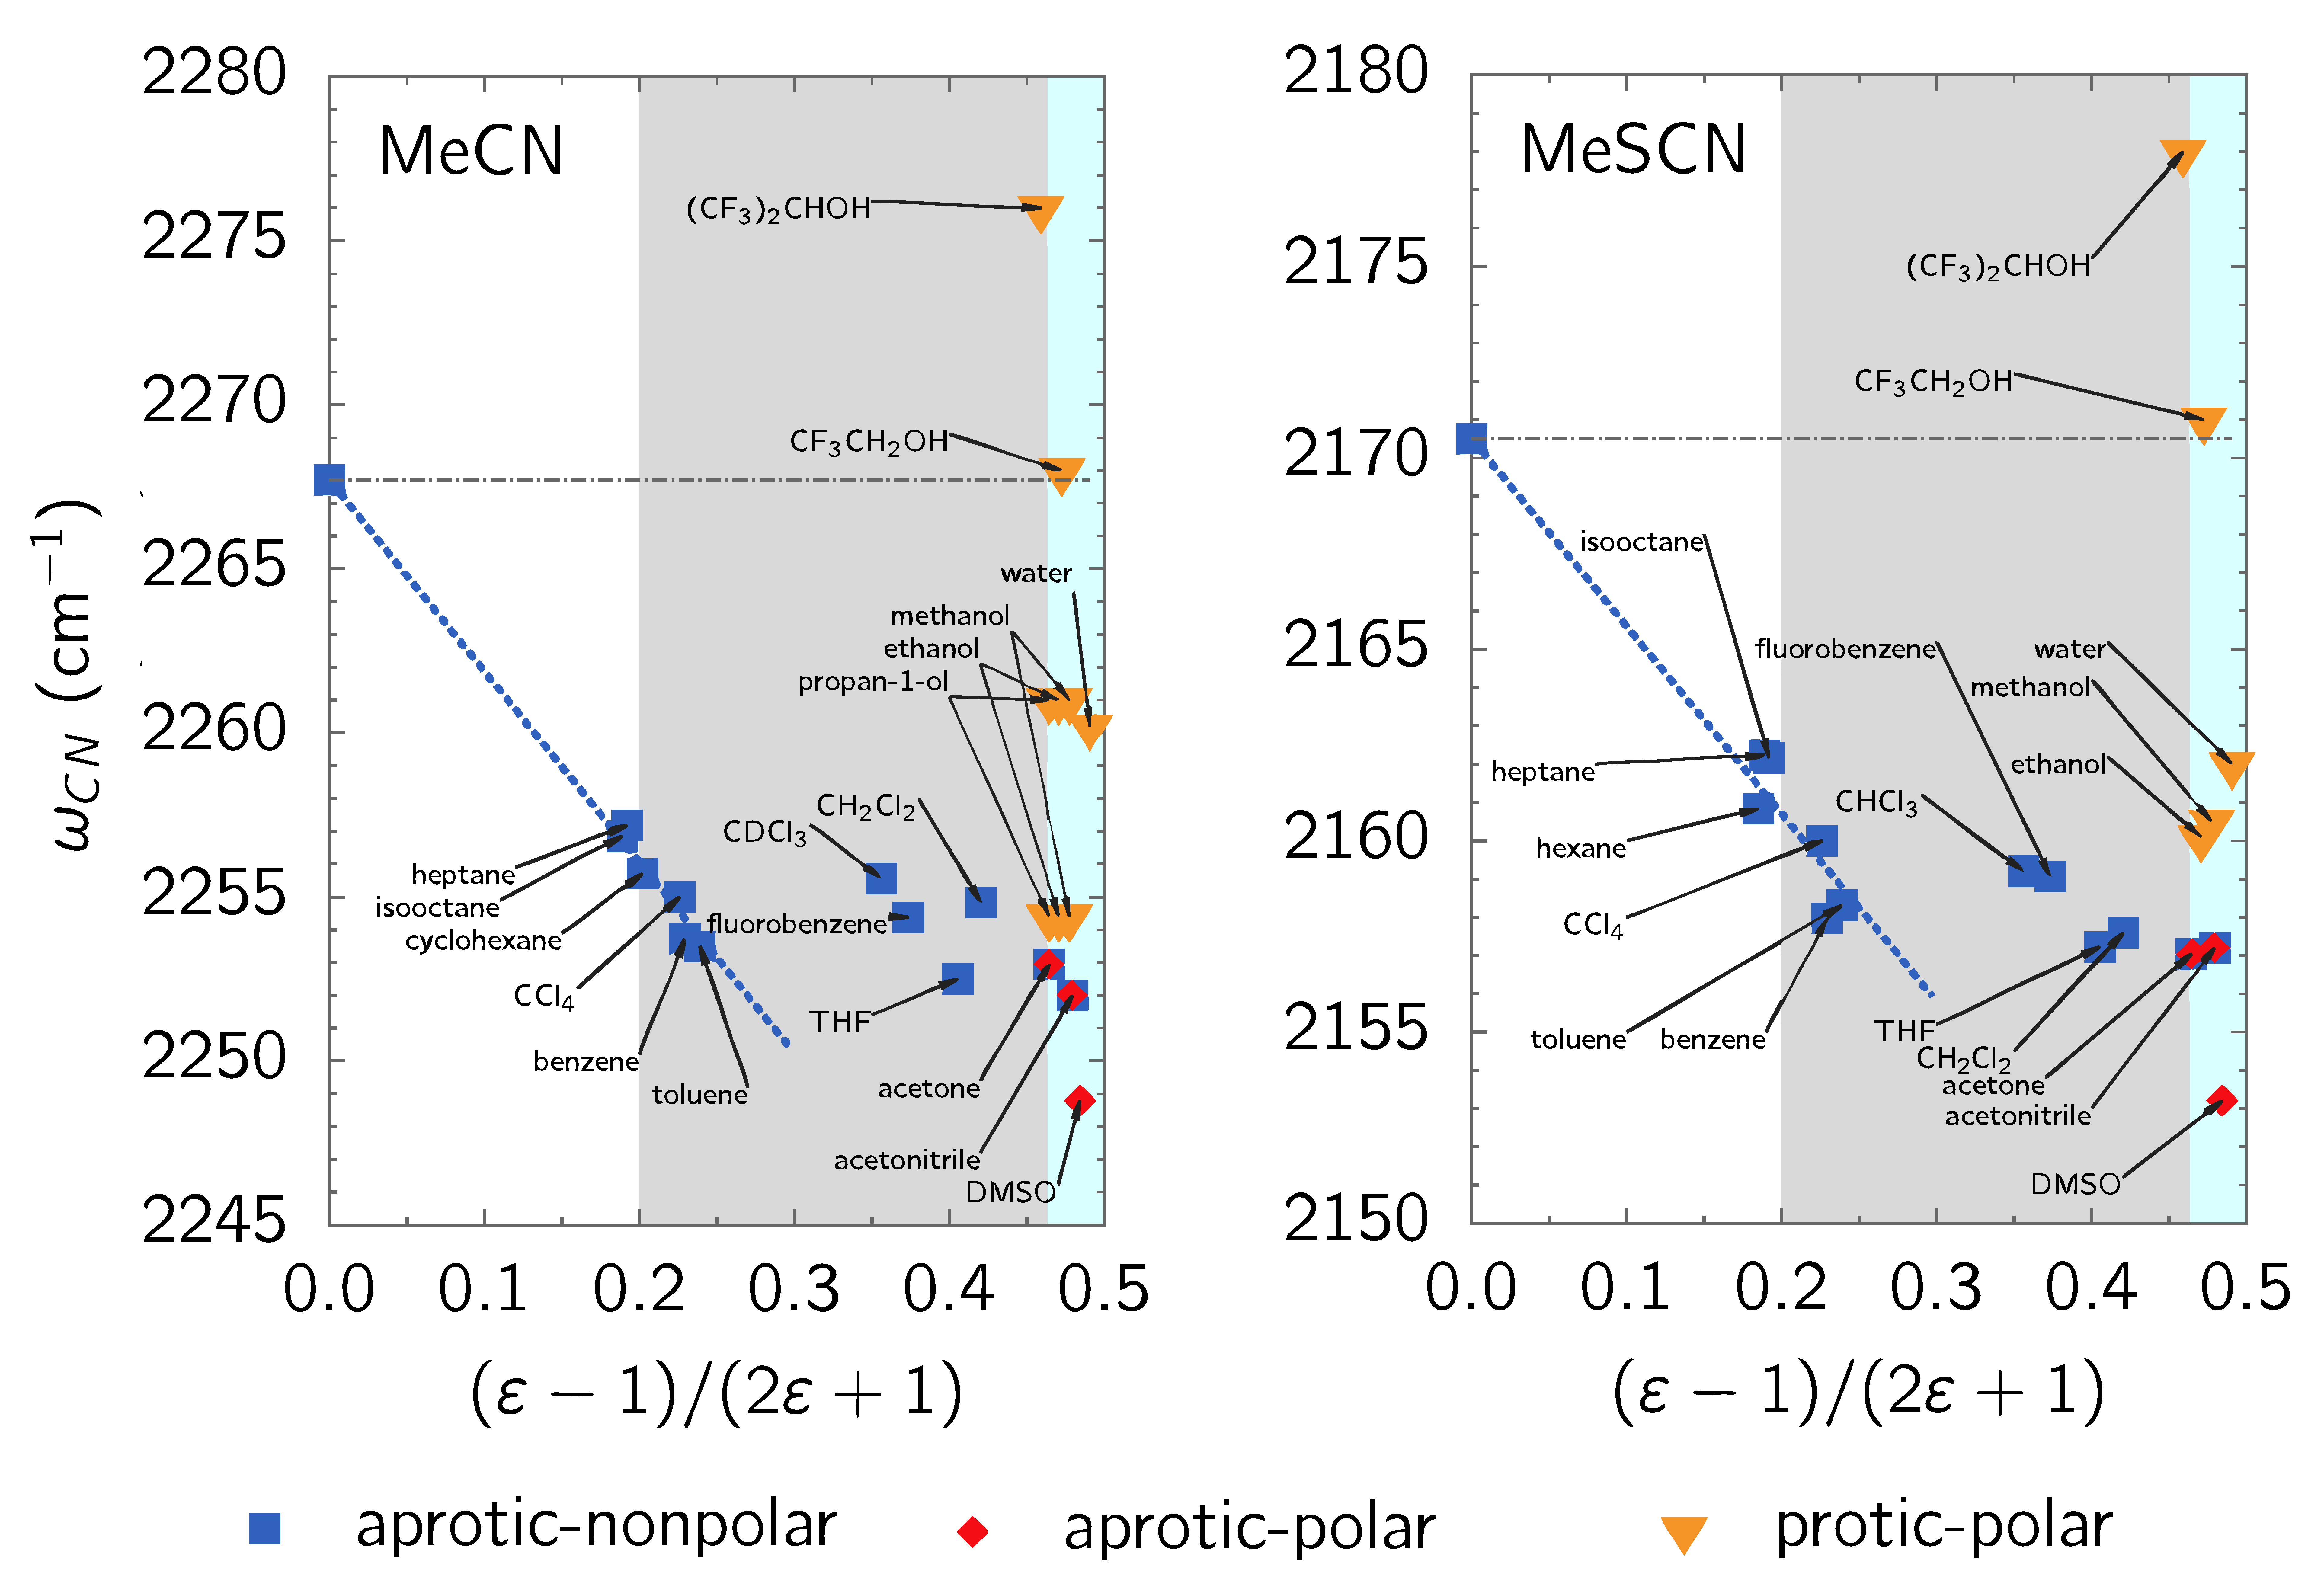
\includegraphics[width=0.9\linewidth]{Fig.1.eps}
}
\caption{Experimental frequencies of CN stretch mode of MeCN and MeSCN dissolved in
various solvents at room temperature. In this Figure, $\varepsilon$
stands for the solvent dielectric constant. Note that Onsager factor is zero in gas-phase. 
Frequencies that were not directly measured for this work were taken from the following 
References: MeCN in gas-phase (Refs.72-74), MeCN in CCl$_4$, THF, MeOH, H$_2$O, CF$_3$CH$_2$OH and 
(CF$_3$)$_2$CHOH (Ref.75), MeCN in CH$_3$(CH$_2$)$_2$OH (Ref.76), MeSCN in gas-phase (Ref.77), MeSCN in 
CCl$_4$, CHCl$_3$, CH$_2$Cl$_2$, MeCN, EtOH, MeOH, H$_2$O, CF$_3$CH$_2$OH and (CF$_3$)$_2$CHOH (Ref.78). In the 
cases of solvents with vanishingly small dipole moment (heptane, hexane, cyclohexane, 
isooctane, CCl$_4$), the linear relationship between CN frequency and Onsager factor indicates that 
the Kirkwood-Bauer-Magat law (blue line) works well.
\label{f.MeCN.MeSCN.vs.solvents}}
\end{figure}
%

As can be seen, for aprotic and non-polar solvents, the linear dependence of
nitrile frequency shift on the Onsager factor is evident, suggesting the validity of the KBM theory.
It is a great success of the apparently simplistic continuum model of solvation. 
However, as the solvent polarity increases, the reaction field 
theory for vibrational solvatochromism fails. Furthermore, as the H-bond donating ability of 
solvent molecule increases, the nitrile stretch frequency becomes strongly blue-shifted, as 
compared to those in DMSO for instance.\citep{Wilderen.Luuk.Kern-Michler.Muller-Werkmeister.Bredenbeck.PCCP.2014}
This just indicates that the continuum representation of the surroundings is not acceptable in general
because of the neglect of the, so called, specific solvation effects. 
They include the direct solute\hyp{}solvent intermolecular
contacts like collisions, directional electrostatic interactions and weak bonding (for instance, hydrogen- (H-) bonding).
Nevertheless, it is clear that vibrational frequency may be fairly sensitive 
to the solvent used, even when the change of the polarity is small.

The solvation of many simple molecules was studied experimentally in detail from the perspective of the 
vibrational properties of some particular localized vibration.\citep{Rowlen.Harris.AnalChem.1991,Mayne.Hudson.JPC.1991,
Janroz.Stangret.Lindgren.JACS.1993,Akiyama.Ohtani.SpectchimActA.1994,
Reimers.Hall.JACS.1999,Wilderen.Luuk.Kern-Michler.Muller-Werkmeister.Bredenbeck.PCCP.2014,Jansen.JPCB.2014} 
Owing to the vibrational solvatochromism
like in Fig.~\ref{f.MeCN.MeSCN.vs.solvents}, 
appropriately chosen vibrational chromophores, which can be either a small molecule or a small functional
group, can be used as a local reporters of their vicinity.\citep{Kim.Cho.ChemRev.2013} 
We shall refer to such interesting chromophores as to the infrared (IR) probes. 

\section{Infrared Probes}

Throughout the years, there have been quite a few IR probes found or synthesized, and
they are nowodays widely used to study various molecular environments, starting from bulk solutions
to proteins, nucleic acids and other polymers.\citep{Kim.Cho.ChemRev.2013,
Ma.Pazos.Zhang.Culik.Gai.AnnuRevPhysChem.2015,Waegele.Culik.Gai.JPCL.2011}
Among the functional gropus that have been demonstrated to be useful IR probes
are carbonyl (CO)\citep{Fried.Bagchi.Boxer.Science.2014,Thielges.Axup.Wong.Lee.Chung.Schultz.Fayer.JPCB.2011}, 
nitrile (CN)\citep{Zhang.Markiewicz.Doerksen.Smith.Gai.PCCP.2015,Johnson.Londergan.Charkoudian.JACS.2014,
Waegele.Culik.Gai.JPCL.2011,Stafford.Ensign.Webb.JPCB.2010,
Silverman.Pitzer.Ankomah.Boxer.Fenlon.JPCB.2007,Suydam.Snow.Pande.Boxer.Science.2006},
asymmetric azide (N$_3$)\citep{Thielges.Axup.Wong.Lee.Chung.Schultz.Fayer.JPCB.2011,
Ye.Zaitseva.Caltabiano.Schertler.Sakmar.Deupi.Vogel.Nature.2010,Waegele.Culik.Gai.JPCL.2011,
Taskent-Sezgin.Chung.Banerjee.Nagarajan.Dyer.Carrico.Raleigh.AngewChemInt.2010,Oh.Lee.Joo.Han.Cho.JPCB.2008} 
stretches, phosphate vibrations\citep{Levinson.Bolte.Miller.Corcelli.Boxer.JACS.2011}
and vibrations within nitro (NO$_2$) group\citep{Smith.Linderman.Luskin.Brewer.JPCB.2011}. 
Unique examples of using simultaneously two localized IR probes
were also reported.\citep{Thielges.Axup.Wong.Lee.Chung.Schultz.Fayer.JPCB.2011}
Those IR probes
generally fulfill the most important requirements for making it a useful tool: i) their transition
frequency is in the spectrally clean region, ii) their oscillatory strength is strong enough
to make them visible in the spectrum and analyze the signal, iii) the line shape 
of the resulting absorption peak is relatively easy to understand and has reasonably
narrow band width. 

Within the carbonyl IR probes, the first ever considered were the amide I modes
naturally occuring in proteins which are mostly the vibrations of the peptide group (CONH). Since
there is a lot of CONH groups in a protein, amide I modes can couple with each other
giving rise to the exciton bands in the IR spectra. This feature enabled to study 
the 3D structures of proteins with a combination of transition density
models\citep{Hayashi.Mukamel.JPCB.2007} because the coupling strongly depends 
on the relative orientation of transition dipoles. 
The problem with amide I mode (or amide I' when the proton becomes deuterated)
is that the linewidth is still relatively broad. In addition, it is impossible to
obtain the local structural information due to the couplings.

Different strategy of using IR probes is related to isolated CO, CN or N$_3$ groups.
CO groups can be genetically encoded
such as CO bound to heme metal center in myoglobin. 
CN and N$_3$ probes can be also site-selectively introduced into a macromolecular 
framework\citep{Jo.Culik.Korendovych.DeGrado.Gai.Biochem.2010,
Wang.Winblade.Johnson.Tirrell.Grabstein.ChemBioChem.2008,Fafarman.Webb.Chuang.Boxer.JACS.2006,
Kiick.Saxon.Tirrell.Bertozzi.PNAS.2002} 
which also provides
a local sond of the molecular environment. In particular, when such IR probe
is inserted into an active site of an enzyme, it becomes possible to study
how the enzyme acts within picosecond time scales.\citep{Fried.Bagchi.Boxer.Science.2014,Bagchi.Boxer.Fayer.JPCB.2012,
Ye.Zaitseva.Caltabiano.Schertler.Sakmar.Deupi.Vogel.Nature.2010} 
Another attractive way is to study protein structural fluctuation dynamics
or the protein-protein contacts when IR probe is localized at the protein 
surface\citep{Taskent-Sezgin.Chung.Banerjee.Nagarajan.Dyer.Carrico.Raleigh.AngewChemInt.2010,
Stafford.Ensign.Webb.JPCB.2010,Oh.Lee.Joo.Han.Cho.JPCB.2008}.  

\section{Understanding the Vibrational Solvatochromism}
%
However, the most fundamental issue that needs to be addressed 
before any IR probe is used, is what actually causes the vibrational solvatochromism.
Definitely, the electrostatic effects were considered to be the most important
(c.f. the KBM model) and much efforts were made to study the effects of the external
electric fields on the vibrational properties.\citep{Kim.Cho.ChemRev.2013} 
In particular, the effects of the
uniform external electric field was thoroughly examined.\citep{Hush.Reimers.JPC.1995,
Reimers.Zeng.Hush.JPC.1996,Andrews.Boxer.JCPA.2002,Cho.JCP.2009} 
In the vibrational Stark spectroscopy (VSE)\citep{Hush.Reimers.JPC.1995,Reimers.Zeng.Hush.JPC.1996}, 
which was pioneered experimentally by Boxer's laboratory\citep{Bublitz.Boxer.AnnuRevPhysChem.1997}, 
the change of the frequency, absorbance
and line shape is measured when the uniform external electric field is applied in certain fixed direction.
Under this circumstance, the frequency shift
was shown to be related to the electric field as follows\citep{Hush.Reimers.JPC.1995,Reimers.Zeng.Hush.JPC.1996}
%
\begin{equation} \label{e:vse-shift-full}
 \Delta \omega \approx - \Delta {\BM \mu} \cdot {\bf F} - \frac{1}{2} \Delta {\BM \alpha} : {\bf F} \otimes {\bf F}
\end{equation}
%
where $\Delta {\BM \mu}$ is, so called, the Stark tuning rate
and $\Delta {\BM \alpha}$ accounts for the quadratic effect with respect to 
the electric field, ${\bf F}$. 
Based on the VSE measurements, for the conventional
electric fields that exist inside biomolecules, the quadratic term
can be safely neglected. 
% CHECK THIS:
%For example, for the maximal electric field
%value reported so far (~160 MV/cm\citep{Fried.Bagchi.Boxer.Science.2014}) and the (assumed) upper bound for 
%$\Delta \alpha=1\times10^{-6}$ 
%cm$^{-1}\times \left({\rm cm}/{\rm MV}\right)^2$\citep{Andrews.Boxer.JCPA.2000,Andrews.Boxer.JCPA.2002}, 
%the frequency shifts is less than 0.03 cm$^{-1}$. For the sake 
%of comparison, the frequency shifts caused by linear term in Eq.~\eqref{e:vse-shift-full}
%can range from 3--100 cm$^{-1}$.
This fact gave rise to the dipole approximation (VSE-d)
widely used by VSE spectroscopists,
%
\begin{equation} \label{e:vse-shift-dipole}
 \Delta \omega \approx - \Delta {\BM \mu} \cdot {\bf F}
\end{equation}
%
Stark tuning rates have been reported for many IR probes.\citep{Suydam.Boxer.Biochem.2003,Levinson.Fried.Boxer.JPCB.2012}
They also were computed by using quantum chemistry calculations\citep{Dalosto.Vanderkooi.Sharp.JPCB.2004,
Andrews.Boxer.JCPA.2002,Andrews.Boxer.JCPA.2000}
and they are typically in a range of 0.4-1.0 cm$^{-1}$/(MV/cm). 
Since Eq.~\eqref{e:vse-shift-dipole} is proportional to solute's
dipole property, VSE-d have been correlated with Onsager's dipole
continuum model. For some subset of aprotic and non-polar
solvents descent linear correlation was found.\citep{Levinson.Fried.Boxer.JPCB.2012} 
Unfortunately,
when strongly protic solvents are used the significant deviations
from the linear correlations were observed.\citep{Fafarman.Sigala.Herschlag.Boxer.JACS.2010,Bagchi.Fried.Boxer.JACS.2012}

However, the serious drawback of VSE lies in the neglect of the field gradients that are 
likely to occur in the condensed phase. In fact, it was denomstrated theoretically
by Cho\citep{Cho.JCP.2009,Lee.Choi.Cho.JCP.2012} 
that when electric field varies in space, Eq.~\eqref{e:vse-shift-dipole}
has to be extended to account properly for field gradients,
%
\begin{equation} \label{e:vse-shift-multipoles}
 \Delta \omega 
\approx 
             - \Delta {\BM \mu}    \cdot               {\bf F} 
- \frac{1}{3}  \Delta {\BM \Theta} :      \nabla       {\bf F}
- \frac{1}{15} \Delta {\BM \Omega} \vdots \nabla\nabla {\bf F}
+ \ldots
\end{equation}
%
where the appropriate \emph{solvatochromic multipoles}
interact with the electric field ($\Delta {\BM \mu}$), 
field gradient ($\Delta {\BM \Theta}$), gradient of field gradient ($\Delta {\BM \Omega}$),
and so forth.
Another problem is related with the crude simplification of the 
molecular surroundings which is treated with continuum Onsager's model.
Despite all that, VSE is still being vividly
used by researchers to probe local electric fields in enzymes, DNA strands and 
lipid layers. 

There is yet another unclear issue which is associated with the electric field
used during the VSE experiment in order to determine Stark tuning rate.
It was shown that actually ${\bf F}$ is not perfetctly constant but varies
near the molecule. The reason for this is the local field effect that arises
from the response of the molecule that is exposed to the perturbing electric field.
This phenomenon is difficult to assess quantitatively. Therefore, 
the empirical scaling factor, so called local field correction factor, $f$, 
was introduced to modify Eq.~\eqref{e:vse-shift-dipole} as follows
%
\begin{equation} \label{e:vse-shift-dipole-corr}
 \Delta \omega \approx - f \Delta {\BM \mu} \cdot {\bf F}
\end{equation}
%
According to continuum Lorentz model, $f$ is given by\citep{Wortmann.Bishop.JCP.1998}
%
\begin{equation}
f(\omega) = \frac{n^2(\omega)+2}{3}
\end{equation}
%
where $n(\omega)$ is the frequency\hyp{}dependent refractive index.
In the limiting case $\omega=0$ $f$ can be also expressed according to Onsager
model as\citep{Wortmann.Bishop.JCP.1998}
%
\begin{equation}
f(0) = \frac{\varepsilon (n^2(0)+2)}{n^2(0)+2\varepsilon}
\end{equation}
%
which extends Lorentz expression by including also orientational polarization effects
but refers to static limit.
It was deduced that $f$ can be in the range of 1.1-1.3\citep{Wortmann.Bishop.JCP.1998,
Bublitz.Boxer.AnnuRevPhysChem.1997}, although
it is unclear whether this is always the case.

It is possible to combine the vibrational spectroscopy of IR probes (mostly VSE) with nuclear magnetic 
resonance (NMR) technique, which was demonstrated by Boxer's 
group.\citep{Fafarman.Sigala.Herschlag.Boxer.JACS.2010,Bagchi.Fried.Boxer.JACS.2012} 
It enables one
to separate out the contributions from the H\hyp{}bonding and other effects. However, 
it is very difficult to use this technique since it refers to empirical observables only,
and hence, one cannot get any detailed insight into the intricacies of the molecular granularity
and types of residues around an IR probe.

A few empirical models of the vibrational solvatochromism has been developed throughout the years.
They employ a variety of fitting procedures with a few adjustable parameters. For example, 
models based on certain molecular descriptors such as polarity, Lewis\slash{}Br{\o}nsted acidity\slash{}basicity, 
H-bonding donating\slash{}accepting ability were shown to be quite useful in relating the vibrational
frequency and infrared intensity with the type of solvent used. Among many methods of this kind,
one can mention Kamlet\hyp{}Taft parameters\citep{Kamlet.Taft.JACS.1976,Taft.Kamlet.JACS.1976,Kamlet.Abboud.Taft.JACS.1977}, 
Fawcett's molecular descriptor method\citep{Reimers.Hall.JACS.1999,
Fawcett.Liu.Kessler.JPC.1993,Fawcett.Kloss.JCP.1996} or Ben Amotz' theory.\citep{Ben-Amotz.Lee.Cho.List.JCP.1992} 
The latter is actually derived from first principles, but it was mostly used by fitting
the resulting parameters to the experiment rather that explicitely obtaining them from calculations.
We will talk about the Ben Amotz' model in more detail later (Section XXX) because it is the first
truly first\hyp{}principles model that decomposes the frequency shifts into not only electrostatic, 
but also non-electrostatic repulsive contributions.

In KT parameter method, frequency shifts can be related to the following
relation\citep{Zhang.Markiewicz.Doerksen.Smith.Gai.PCCP.2015}:
%
\begin{equation} \label{e:kamlet-taft}
\Delta \omega = A\alpha + B\beta + C\pi^{*}
\end{equation}
%
In this approach, one has to
find the coefficients $A$, $B$ and $C$ that are fitted against
the solute's KT parameters $\alpha$\citep{Taft.Kamlet.JACS.1976}, 
$\beta$\citep{Kamlet.Taft.JACS.1976} and $\pi^{*}$\citep{Kamlet.Abboud.Taft.JACS.1977} 
describing the hydrogen bond accepting,
hydrogen bond donating, and dielectric interactions abilities, respectively.
KT parameters were originally determined from VIS spectra and related different
spectroscopic observables into one multivariate linear relationship as in Eq.~\eqref{e:kamlet-taft}.

Slightly more complicated parameterization was developed 
by Fawcett et al.\citep{Reimers.Hall.JACS.1999,Fawcett.Liu.Kessler.JPC.1993,Fawcett.Kloss.JCP.1996},
in which the solute's frequency shift\footnote{originally acetonitrile $\nu_2$ frequency
which is CN stretch mode} can be expressed by the mix of solute- and
solvent-related empirical descriptors
%
\begin{multline} \label{e:fawcett}
\Delta \omega = \Delta \omega_{gp} + 
\left( a_{Sol} - a_{St} \right) A_A +
\left( d_{Sol} - d_{St} \right) A_D \\ + 
\left( \frac{\varepsilon_{Sol}-1}{\varepsilon_{Sol}+2} - \frac{\varepsilon_{St}-1}{\varepsilon_{St}+2} \right) A_\varepsilon +
\frac{3}{4\pi}
\left( \frac{n^2_{Sol}-1}{n^2_{Sol}+2} - \frac{n^2_{St}-1}{n^2_{St}+2} \right) A_\alpha
\end{multline}
%
In the above formula, $\Delta \omega_{gp}$ denotes the frequency shift in pure liquid of solute
relative to the gas phase,
$a$ and $d$ are the Gutmann solvent acceptor and donor numbers\citep{Gutmann.Resch.Linert.CoordChemRev.1982}, 
respectively,
and the associated four constants $A_A$, $A_D$, $A_\varepsilon$ and $A_\alpha$ 
are to be fit to the experimentally determined frequency shifts in different solvents.
The lower indices $St$ and $Sol$ indicate solute and solvent parameters, respectively. 
Note that all fitting parameters in Eqs.~\eqref{e:kamlet-taft} and ~\eqref{e:fawcett} 
describe the solute-solvent interactions empirically.

In his seminal works, Ben-Amotz et al.\citep{Ben-Amotz.Lee.Cho.List.JCP.1992} 
used the first-principles theory of Buckingham\citep{Buckingham.ProcRSocLondonA.1958,
Buckingham.ProcRSocLondonA.1960,Buckingham.TransFaradaySoc.1960}
to derive the contributions to the vibrational frequency shift due to
repulsive, attractive and centrifugal distortion forces. Mainly,
%
\begin{equation} \label{e:ben-amotz}
 \Delta \omega = \Delta \omega_R + \Delta \omega_A + \Delta \omega_C
\end{equation}
%
It was concluded that the repulsive part $\Delta \omega_R$ is more or less constant
and constitutes about 4 cm$^{-1}$ to the blue shift. Attractive part, $\Delta \omega_A$,
was attributed to the dispersion and dipole-dipole interactions
and was shown to be proportional to the solvent density as
%
\begin{equation} \label{e:ben-amotz-ro}
 \Delta \omega = 2\pi\left( A_\alpha \alpha_S + A_\mu \mu_S^2 \right) \rho_S
\end{equation}
%
in which constants $A_\alpha$ and $A_\mu$ could be determined empirically. 
In the above equation, $\rho_S$ is the solvent density whereas $\mu_S$ and $\alpha_S$ are the
dipole moment magnitude and isotropic polarizability of the solvent molecules.

The centrifugal distortion effect on acetonitrile CN stretch frequency 
caused by inhibited rotation of solute molecules
in solution was estimated to be roughly --0.5 cm$^{-1}$ in the liquid phase.  
The empirical relationship in Eq.~\eqref{e:ben-amotz-ro} was proven to be not sufficient to obtain 
satisfactory correlations with experiment and more refined
models (such as Fawcett et al.'s model) were necessary.\citep{Reimers.Hall.JACS.1999} 
Nevertheless, 
to the best of my knowledge, both the theory of Ben-Amotz et al.\citep{Ben-Amotz.Lee.Cho.List.JCP.1992} 
and the theory
developed later in this Thesis are the only first-principles theories on the
vibrational solvatochromism that explicitly take into account the electrostatic 
attractive and non-Coulombic repulsive interactions.

Another important class of empirical or semi\hyp{}empirical methods which is broadly reffered 
to as the electrostatic fitting methods (ESF), uses the correlation of benchmark 
\emph{ab initio} or density functional theory (DFT)-calculated vibrational properties
with electrostatic potential, electric field or its gradients, that are estimated at various
points in space around an IR probe. 
The method can be generally described by the following empirical relationship
%
\begin{equation} \label{e:esf}
 P(\phi \text{ or } {\bf F}) = \sum_X \left\{ l_X \phi_X + {\bf d}_X \cdot {\bf F}_X + {\bf D}_X : \nabla{\bf F}_X \right\}
\end{equation}
%
where $P$ is the property in question (frequency, transition dipole and so on), 
$\phi_X$ and ${\bf F}_X$ are the electrostatic potential and electric field, respectively, that are
evaluated at some point $X$.
These points are called 'interaction centers' and their
choice is mostly a matter of pure convenience in order to obtain a reliable and efficient
fitting model ($l_x$, ${\bf d}_x$, ${\bf D}_x$ parameter set). Mostly, only one type of parameters
(e.g. scalar by Cho's group or vector by Skinner's group) is employed, but there are also maps utilizing multiple types of parameters
as well (scalar + vector by Torii's group or vector + vector gradient by Jansen et al.).
 
In practice, the spectator molecule in question is either solvated by a relatively small number of polar 
solvent molecules that create varying electrostatic potential. The perturbing fields can also be applied directly
in many directions. It is also possible to account for molecular anharmonicity
when the model gas\hyp{}phase Hamiltonian with polynomial expansion of anharmonic potential
is used and perturbed by external electric fields.
Subsequent multivariate
least-square analyses of these model systems are then performed to obtain the vibrational 
solvatochromic parameters (or maps) for a given IR probe molecule, from which the benchmark
results could be reproduced. 

Despite it was reported that ESF approach can be very accurate in reproducing the frequency shifts and even
transition dipoles, we pointed out that the fitting procedures
can be biased towards a chosen subset of systems or molecular environments. This obvously can limit
the transferability and universality of the method, unless the reference data is 'complete enough'
to cover all relevant solute-solvent interaction scenarios. Note that the ESF approach intrinsically
assumes that the only driving force of the vibrational solvatochromism is \emph{electrochromism}
and all other aspects of intermolecular interactions like van der Waals forces and charge transfer are
ignored in the theoretical formulation. On the other hand, since ESF is based on fitting, it is 
possible that also non\hyp{}electrostatic effects are captured by this method when calculating the benchmark 
vibrational frequencies of solute-solvent clusters. This may cause serious problems with the interpretations
of the frequency shifts based on ESF. If non\hyp{}electrostatic contirbutions affect the fitting
parameters, the conclusions about the structural features of the systems will be incorrect 
because ESF assumes electrostatic functional form (strongly solute-solvent orientation-dependent).\footnote{
The same problem refers to VSE-d approximation from Eq.~\eqref{e:vse-shift-dipole-corr}.
If there are other terms contributing to frequency shift like quadrupolar terms 
in Eq.~\eqref{e:vse-shift-multipoles} the conclusions based
on the analysis of VSE data are incorrect.}

There are a few reports showing that the ESF parameters can achieve the level of solvent
and even solute transferability. However, it is not at all clear to what extent the universality is
preserved, especially when the change of environment is drastic. For example, let us consider putting a probe in
a completely non-polar solvent such as CCl$_4$ which has no net molecular dipole moment. 
Then, let us apply an ESF map that was derived in aqueous solutions (which is mostly the case in this kind
of parameterizations). Since CCl$_4$ molecules are rather unlikely to exert strong electrostatic fields 
around IR probe we might expect very small frequency shifts. But the examples of MeCN and MeSCN probes
dissolved in this solvent (Fig.~\ref{f.MeCN.MeSCN.vs.solvents}) show the very pronounced frequency red shifts that are roughly -10 cm$^{-1}$
relative to the gas phase, which is comparable to frequency shifts in water! 
We will show later that it is basically impossible by using a purely electrostatic approach
to capture these misterious effects that cause so strong red shifts in the case of CN stretch in non-polar
solvent. It is also not so clear whether electorstatic map from Eq.~\eqref{e:esf} is able to 
encapsulate those effects into the fitting parameters.

It is also possible to use experimentally measured protein spectra directly as reference data. 
Such an approach is specifically designed for dealing with very large systems like proteins and
can be very accurate. Unfortunately, it provides no physical interpretation of the observed
spectral signals and has only predictive power.

\section{Signs of Non-Electrostatic Vibrational Solvatochromism}
As opposed to the bunch of studies concentrating on the electrostatic
approximation of the vibrational solvatochromism, there exist a few 
semi-empirical works of the other effects that trigger frequency shift
changes upon solvation. 

Perhaps one of the first was the study of Ben Amotz et al in 1991.
They wanted to understand the relationship between the vibrational frequency
and the pressure. The first\hyp{}principles model built on the Buckingham's theoretical
foundations was used to obtain the empirical set of parameters fit to
experimental data of chosen vibrational frequencies in various solvents
and pressures.

In 1998, Reimers and Hall investigated in great detail the solvation of acetonitrile 
based on the Ben Amotz and Fawcett models. It is surprising to me what they found.
From among 33 various solvents ranging from non-polar and non-protic CCl$_4$, through strongly protic
DMSO to quite acidic trifluoroacetic acid (TFA), they noticed that the electrostatic
non-specific interactions cause much lesser redshifts as compared to the dispersion
interactions. Note that the latter cannot be correlated with electrostatic potential
or electric field at all. What is also interesting in their work is that they 
reported specific (short\hyp{}range) frequency \emph{blue shifts} which were strongly enforced
in solvents forming H-bonding interactions. In fact, the stronger H-bonds formed between MeCN
and solvent molecules, the larger this blue shift was obtained.

Since, at that time it was impossible to discriminate between various short-range
interactions, the physical nature of the misterious blue shifts remained unknown.
However, there appeared other theoretical analyses of the CN frequency shifts of MeCN in water
or CN$^-$ anion in water. Rey and Hynes\citep{Rey.Hynes.JCP.1998} decomposed the forces obtained from classical molecular dynamics
(CMD) simulations and found that the van der Waals potential exerts strong blue shifts of CN mode in CN$^-$.
Similar conlcusion was drawn by Morales and Thompson who investigated MeCN/water system by 
using CMD. 

The signs of non-negligible exchange-repulsion-induced frequency shifts were 
investigated by Wang, XX and XX. They showed indirectly, by correlating the interaction
energy components from symmetry-adapted perturbation theory (SAPT) with frequency shifts, that repulsive potentials
lead to blue shifts. Rodziewicz et al. used similar approach studying the series of 
blue\hyp{} and red\hyp{}shifting complexes. They found similar conclusion and attributed the
blue shifting patterns to the 'repulsion wall' caused by Pauli exlusion principle. 
Also, they noticed that
the dispersion effects can affect the vibrational frequency in various ways
and discriminated between two distinct mechanisms.

In 2005, Zierkiewicz has combined Buckingham's theory for a diatomic case approximation with SAPT 
and studied vibrations involving C--H or C--X
stretches, where X denotes halogen atom. They found that the exchange-repulsion effects
cause blue shifts and the nature of these frequency shifts is quite complex. Also, dispersion
interation\hyp{}induced red shifts were non-negligible.

In 2009, Choi et al were studying the effects of charge transfer on the vibrational
frequency of the model ionic IR probes such as CN$^-$ or N$_3^-$ anions dissolved in water. 
Although they found a considerable charge
transfer between solute-water molecules, the total charge transferred appeared to be in no
correlation with the vibrational frequency shifts. This was interpreted that the charge transfer 
phenomenon can be neglected when considering the vibrational interaction-induced frequency shifts
for the studied systems. However, charge transfer was found to be almost as important as electrostatic
interactions in the recent work of Brizner et al., in which they studied CO$_2$ assymetric
stretching ($\nu_3$) mode as an IR probe for sensing the local molecular environments in ionic
liquids.

In the forthcoming Chapters we will present the detailed fully first-principles expressions
that can be used to calculate various contributions to the vibrational solvatochromic frequency
shifts directly by means of quantum chemistry calculations. We also test these quations 
and when combined with CMD we show that such a theory can quantitatively predict the
vibrational solvatochromism of many IR probes.

\printbibliography[heading=subbibintoc,title={References}]
\end{refsection}

% ==== CHAPTER 2

\begin{refsection}
\chapter{Vibrational Solvatochromism Theory\label{c:background}}

As pointed out in previous Chapter, understanding the vibrational
solvatochromism requires a rigorous quantum mechanical treatment.
In this Chapter, we derive the fundamental theories of the vibrational
solvatochromism by analyzing the Hamiltonian of an IR spectator molecule.
The frequency shift and transition dipole are then expressed as functions
of the solute-solvent interaction potentials.

\section{Overview\label{s:theory}}

The rigorous first\hyp{}principles theory behind the vibrational solvatochromism was published
for the first time by Buckingham.\citep{Buckingham.TransFaradaySoc.1960} 
In his seminal works, Buckingham found the fundamental 
relation between the solute\hyp{}solvent interaction energy change along normal 
coordinates, solute's anharmonicity and the vibrational frequency shifts.
His formula, although derived for the general $N$-atomic case, was tested
only for the diatomic approximation. His theory was found to predict not only
the interaction\hyp{}induced frequency shift, but also structural deformation in simple
diatomic cases.

In 1980s, Hush and Reimers were considering the vibrational electrochromism
to quantitatively relate $\Delta \omega$ with the external electric fields.

The theory was rediscovered later by Cho, though using different theoretical
approach, he found essentially the same formulas for the frequency shifts as Buckingham, Hush
and Reimers. However, Cho's 
approach focused on more practical application of the vibrational solvatochromism 
theory and enabled fragment\hyp{}based approach to this problem. In his coarse-grained
model of vibrational solvatochromism, he showed that,
under electrostatic approximation based on the distributed multipole expansion, 
$\Delta \omega$ can be written in an analogous manner as the conventional
Coulomb interaction energy. He constructed the first-principle set of 
the \emph{solvatochromic multipole moments} that can be systematically used
to predict the electrostatic frequency shifts. Thus, this work opened a new route for developing
all-encompassing theory based on single molecules, which is based not just on
Coulomb interactions, but includes other intermolecular forces alltogether.

The theoretical dissertations of Buckingham and Cho were my stimuli and inspired
me to extend the coarse\hyp{}grained electrostatic vibrational solvatochromism 
model of Cho by the analysis of the other fundamental intermolecular interactions.
%exchange-repulsion, induction (polarization), dispersion and charge transfer (CT).
Therefore in the forthcoming sections, we will go through both of the models in detail
to derive the ab initio expressions for the interaction-induced 
vibrational frequency shifts that are not limited by electrostatic approximation.
The Reader who is not familiar with the theory of vibrations is strongly encouraged
here to first read the Appendix~\ref{a:vibrational-analysis} (especially Section~\ref{a:harmonic-oscillator})
in which the brief introduction to this fundamental aspect is presented.

\section{Buckingham's model  \label{s:buckingham-theory}}

The starting point in Buckingham's consideration was to consider 
the harmonic oscillator Hamiltonian which is perturbed by anharmonicity
and the interaction potential between solute and solvent molecules. Mainly,
%
\begin{equation}
\mathscr{H} = \mathscr{H}_{\rm Harm} + \mathscr{H}_{\rm Anh} + U({\bf Q}_A,{\bf Q}_B)
\end{equation}
%
where
%
\begin{equation}\label{e:h_harm}
\mathscr{H}_{\rm Harm} = 
\sum_j \frac{\mathscr{P}_j^2}{2M_j} + \frac{1}{2} M_j \omega_j^2 Q_j^2
\end{equation}
%
and
%
\begin{equation}\label{e:h_anh}
\mathscr{H}_{\rm Anh} = 
\sum_{ijk} \frac{1}{3!} g_{ijk} Q_iQ_jQ_k + \ldots 
\end{equation}
%
where $Q_i$ denotes the $i$th normal coordinate of the solute in gas phase whereas
${\bf Q}_A$ and ${\bf Q}_B$ represent the structures of solute and solvent, 
respectively.

The solutions to the Schr{\"o}dinger equations for the solvated and 
unsolvated states can be written as
%
\begin{eqnarray}
\left[ \mathscr{H}_{\rm Harm} + \mathscr{H}_{\rm Anh} + U \right] 
\vert \Psi \rangle &=& W \vert \Psi \rangle \\
\left[ \mathscr{H}_{\rm Harm} + \mathscr{H}_{\rm Anh} \right] 
\vert \Gamma \rangle &=& G \vert \Gamma \rangle 
\end{eqnarray}
%
with $\vert\Psi\rangle$ and $\vert\Gamma\rangle$ representing the solute's wavefunctions
in its solvated and gas-phase states, respectively.

Since the exact solutions of the Schr{\"o}dinger equations are known 
for $\mathscr{H}_{\rm Harm}$, Buckingham used the perturbation theory
to derive the effects on the vibrational energies upon binding with solvent
molecule (here abbreviated as $B$).
In other words, he assumed that
%
\begin{equation} \label{e:RSPT-Hamiltonian}
\mathscr{H} = \mathscr{H}^{(0)} + \mathscr{H}'
\end{equation}
%
where the zeroth\hyp{}order Hamiltonian $\mathscr{H}^{(0)}=\mathscr{H}_{\rm Harm}$
and the perturbation operator $\mathscr{H}'=\mathscr{H}_{\rm Anh} + U({\bf Q}_A,{\bf Q}_B)$.
The zeroth-order energies are given by
%
\begin{equation}
E_{n,j}^{(0)} = \hbar \omega_j \left( n_j+\frac{1}{2} \right)
\end{equation}
%
Since the series expansions along $Q_i$ are used in Eqs.~\eqref{e:h_harm}
and~\eqref{e:h_anh}, the solute\hyp{}solvent interaction potential
should also be expanded:
%
\begin{equation}\label{e:u_taylor}
U({\bf Q}_A,{\bf Q}_B) = 
U_0 + \sum_j \frac{\partial U}{\partial Q_j} \Bigg|_{{\bf Q}_{0_A}}
+ \frac{1}{2} \sum_{ij} \frac{\partial^2 U}{\partial Q_i \partial Q_j} \Bigg|_{{\bf Q}_{0_A}}
+ \ldots
\end{equation}
%
where $U_0$ is a constant offset. 

To estimate the frequency shifts, one has to study the changes
in the vibrational energy levels after the solute\hyp{}solvent 
interaction potential is turned on. Up to the second order
of the Reighleigh\hyp{}Schr{\"o}dinger perturbation theory (RSPT), 
the energy of the solvated ($W$) and unsolvated ($G$) 
$n$th vibrational state of $j$th normal mode can be expressed as
%
\begin{eqnarray}\label{e:gwlevels}
W_{n,j}^{(2)} &= E_{n,j}^{(0)} + \delta W_{n,j}^{(1)} + \delta W_{n,j}^{(2)} \\
G_{n,j}^{(2)} &= E_{n,j}^{(0)} + \delta G_{n,j}^{(1)} + \delta G_{n,j}^{(2)}
\end{eqnarray}
%
in which the $\delta$ symbol denotes the corresponding RSPT correction. Note 
that the perturbations associated with $W$ and $G$ differ only by 
the additional $U$ term. 

Before we start the rigorous derivations, we need first to set up the appropriate labeling system
for the complicated vibrational states of the polyatomic molecule which has many normal modes.
In this Work, we will consider only vibrational energy levels that are associated with
the excitation of a single normal mode $j$, i.e., we restrict the analysis to the fundamental
and overtone transitions. In such a case, the 
wavefunctions can be schematically represented by
%
\begin{eqnarray}
\vert \Psi_{j_n}   \rangle &= \vert 1_0 2_0 \ldots j_n \ldots \rangle_{\Psi} \\
\vert \Gamma_{j_n} \rangle &= \vert 1_0 2_0 \ldots j_n \ldots \rangle_{\Gamma} 
\end{eqnarray}
%
where $j_n$ denotes the $n$th vibrational energy level of the $j$th normal mode.
Moreover, we shall assume that the general vibrational 
eigenstate can be represented by a vector spanned
in a \emph{composite} Fock space constructed from subspaces corresponding 
to separate 1\hyp{}dimensional oscillators. Mainly,
%
\begin{equation}  \label{eq:general_state_vibr}
\vert S_{1_k2_l\cdots j_n\cdots}   \rangle 
 \cong \vert 1_k \rangle \otimes \vert 2_l \rangle \otimes \cdots \vert j_n \rangle \otimes \cdots 
\end{equation}
%
In a similar fashion as above, the composite displacement operators $Q_j$
are understood as
%
\begin{equation}
Q_j \rightarrow \mathbb{I}_1 \otimes \mathbb{I}_2 \otimes \cdots Q_j \otimes \cdots
\end{equation}
%
which means that only $j$th normal coordinate is displaced leaving the others
in their equilibrium values (identity operators $\mathbb{I}_k$ do not change $k$th mode).

Note that the above approximations are exact only in the case of 
fully harmonic system because the notion 'normal mode' refers to
the isolated harmonic oscillator, even if seen in a more general context
when anharmonicity and vibrotational couplings are included as well.
However, we are going to use RSPT based on harmonic oscillators as 
sets of reference states. In such a case, Eq.~\eqref{eq:general_state_vibr} 
can be used.

Now let us return to the derivation of the vibrational frequency shifts. 
By considering the gas phase states it is easy to see that 
$\delta G_{n,j}^{(1)}$ vanishes,
%
\begin{equation}
\delta G_{n,j}^{(1)} = \frac{1}{6}\sum_{ijk} g_{ikl} 
\langle \Psi_{j_n} \vert Q_iQ_kQ_l \vert \Psi_{j_n} \rangle = 0
\end{equation}
%
because all the diagonal matrix elements of $Q_i$ and $Q_i^3$ operators
are zero (see the Appendix~\ref{a:matrix-elements}).
The second-order correction is 
%
\begin{equation}
\delta G_{n,j}^{(2)} = \frac{1}{6^2} \sum_{S}{^{'}} \sum_{ikl}\sum_{i'k'l'} g_{ikl} g_{i'k'l'}
\frac{\langle \Psi_{j_n} \vert Q_iQ_kQ_l \vert S \rangle \langle S \vert Q_{i'}Q_{k'}Q_{l'} \vert \Psi_{j_n} \rangle }
{ E_{n,j}^{(0)} - E_{S}^{(0)} }
\end{equation}
%
where the primed sum over $S$ ensures that $\vert S \rangle \ne \vert \Psi_{j_n} \rangle$. 
It is clear that $\delta G_{n,j}^{(2)}$ is quadratic with respect to the cubic anharmonic constants.
Therefore, it is relatively small and we will neglect this contribution.
To sum up, the gas phase energy levels can be thought of as just 
harmonic vibrational levels:
%
\begin{equation}\label{e:ge}
G_{n,j}^{(2)} \approx E_{n,j}^{(0)}
\end{equation}
%
When the $U$ operator is added to the perturbation, it adds the linear
and quadratic terms with respect to the interaction energy derivatives and therefore
the corrections $\delta W_{n,j}^{(1)}$ and $\delta W_{n,j}^{(2)}$ 
are non\hyp{}negligible anymore.

\subsection{First-order frequency shift}

From Eqs.~\eqref{e:gwlevels} and~\eqref{e:ge} it implies that 
the first\hyp{}order frequency shift corresponding to the transition
$n\leftarrow m$ 
is proportional to the difference between the first-order corrections 
$\delta W_{n,j}^{(1)}$ and $\delta W_{m,j}^{(1)}$. That is
%
\begin{equation}\label{e:dw-first-order-pt}
\delta \omega_{n\leftarrow m,j}^{(1)} = 
\frac{1}{\hbar} 
\left( \delta W_{n,j}^{(1)} - \delta W_{m,j}^{(1)} \right)
%- \omega_{nm,j}^{0}
\end{equation}
%
where
%%
%\begin{equation}
%\omega_{nm,j}^{0} = (n-m)\omega_j
%\end{equation}
%
%and
%
\begin{equation}
\delta W_{n,j}^{(1)} = \langle \Psi_{j_n} \vert \mathscr{H}' \vert \Psi_{j_n} \rangle
\end{equation}
%
By a careful examination of the matrix elements one finds that
%
\begin{equation}
\delta W_{n,j}^{(1)} = U_0 + \frac{1}{2} 
\left[ 
                  \langle j_n \vert Q_j^2 \vert j_n \rangle \frac{\partial^2 U}{\partial Q_j^2} \Bigg|_{{\bf Q}_{0_A}}
  + \sum_{i\ne j} \langle i_0 \vert Q_i^2 \vert i_0 \rangle \frac{\partial^2 U}{\partial Q_i^2} \Bigg|_{{\bf Q}_{0_A}}
\right]
\end{equation}
%
Substituting this into Eq.~\eqref{e:dw-first-order-pt} we have
%
\begin{equation}
\delta \omega_{n\leftarrow m,j}^{(1)} = 
\frac{1}{2\hbar}  \frac{\partial^2 U}{\partial Q_j^2} \Bigg|_{{\bf Q}_{0_A}}
\left[
    \langle j_n \vert Q_j^2 \vert j_n \rangle - \langle j_m \vert Q_j^2 \vert j_m \rangle 
\right]
\end{equation}
%
Using the fact that $\langle j_n \vert Q_j^2 \vert j_n \rangle=\hbar(2n+1)/2M_j\omega_j$
we finally get the exression for the first\hyp{}order frequency shift involving $n\leftarrow m$
transition
%
\begin{equation}
\label{e:buckingham-1st-order}
\boxed{
\delta \omega_{n\leftarrow m,j}^{(1)} = \left( \frac{n-m}{2M_j\omega_j} \right) 
\frac{\partial^2 U}{\partial Q_j^2} \Bigg|_{{\bf Q}_{0_A}}
}
\end{equation}
%
For the special case of the $1\leftarrow 0$ (fundamental) transitions, the frequency
shift is
%
\begin{equation}
\label{e:buckingham-1st-order-fundamental}
\delta \omega_{1\leftarrow 0,j}^{(1)} =  \frac{1}{2M_j\omega_j}
\frac{\partial^2 U}{\partial Q_j^2} \Bigg|_{{\bf Q}_{0_A}}
\end{equation}
%
Note also that $\delta \omega_{(m+1)\leftarrow m,j}^{(1)} = \delta \omega_{m\leftarrow (m-1),j}^{(1)}$
and, in particular, the anharmonicity of the vibrational degree of freedom is \emph{constant}
up to the first\hyp{}order perturbation. That is,
%
\begin{equation}  \label{e:anharm-1st-order}
\delta^{(1)} \Delta_{\rm Anh} \equiv \Delta^{(1)} (\omega_{1\leftarrow 0,j} - \omega_{2\leftarrow 1,j}) = 0
\end{equation}
%

\subsection{Second-order frequency shift}

From Eqs.~\eqref{e:gwlevels} and~\eqref{e:ge}, the second-order 
frequency shift corresponding to the $n\leftarrow m$ transition 
is given by
%
\begin{equation}\label{e:dw-second-order-pt}
\delta \omega_{n\leftarrow m,j}^{(2)} = 
\frac{1}{\hbar} 
\left( \delta W_{n,j}^{(2)} - \delta W_{m,j}^{(2)} \right)
\end{equation}
%
where
%
\begin{equation}\label{eq:domega2}
\delta W_{n,j}^{(2)} = \sum_{S}{^{'}}
\frac{
   \langle \Psi_{j_n} \vert \mathscr{H}' \vert S          \rangle
   \langle S          \vert \mathscr{H}' \vert \Psi_{j_n} \rangle
}{E^{(0)}_{n,j} - E^{(0)}_S}
\end{equation}
%
By a more careful analysis of the terms in the numerator of
Eq.~\eqref{eq:domega2} one can notice that the leading terms
will be the ones that are first order in $U$ and third-order 
in $g$. Therefore 
%
\begin{equation}\label{eq:domega2approx}
\delta W_{n,j}^{(2)} \cong 
\frac{1}{3}
\sum_{S}{^{'}}
\sum_{ijkl}
\frac{
   \langle \Psi_{j_n} \vert Q_i \vert S          \rangle
   \langle S          \vert Q_jQ_kQ_l \vert \Psi_{j_n}  \rangle
}{E^{(0)}_{n,j} - E^{(0)}_S} U_{0,i} g_{jkl}
\end{equation}
%
This expression seems to be still very complex. However, due to the multiplication of each 
third-order matrix element by a first-order matrix element, the summation
over $S$ is dramatically restricted only to a very small subset of states.
Note that if $i=J$ then all vibrational states corresponding to normal coordinate
other than $J$ need to be zero due to the orthogonality of the harmonic oscillator
eigenstates. Moreover, states corresponding to the normal coordinate $J$ are restricted 
to only two possible
vibrational energy states that give non-zero integral, i.e., $n_J \pm 1$ (see Appendix).
In the case when $i\ne J$ in the summation, then only $J_n$ and $i_1$ quantum numbers will 
survive. Therefore
%
\begin{multline}  \label{eq:1x3}
\delta W_{n,j}^{(2)} =
\frac{1}{3}
\sum_{m_J= n_J \pm 1} 
\sum_{jkl}
\frac{
   \langle \Psi_{J_n} \vert Q_J \vert \Psi_{J_m}          \rangle
   \langle \Psi_{J_m} \vert Q_jQ_kQ_l \vert \Psi_{J_n}  \rangle
}{\hbar \omega_J (n_J-m_J) } U_{0,J} g_{jkl}                    \\
%
- \frac{1}{3}
\sum_{i\ne J}
\sum_{jkl}
\frac{
   \langle \Psi_{J_n} \vert Q_i \vert \Psi_{i_1J_n}          \rangle
   \langle \Psi_{i_1J_n} \vert Q_jQ_kQ_l \vert \Psi_{J_n}  \rangle
}{\hbar \omega_i } U_{0,i} g_{jkl}                    
\qquad
\end{multline}
%
where we denoted symbolically $\vert \Psi_{i_1J_n} \rangle$ the states 
with the first excited level for $i$th mode and $J_n$ state for the $J$th mode.

Let us first analyze the first summation term appearing in Eq.~\eqref{eq:1x3}.
By explicitely expanding the summation over vibrational levels and subsequent resolving
the matrix elements we are led to the following:
%
\begin{multline}
\frac{1}{3}  \sum_{jkl}
  \Bigg\{ 
   \frac{\langle n_J \vert Q_J \vert n_J+1 \rangle 
         \langle n_J+1 \vert Q_jQ_kQ_l \vert n_J \rangle}{\hbar \omega_J} \\
 - \frac{\langle n_J \vert Q_J \vert n_J-1 \rangle
         \langle n_J-1 \vert Q_jQ_kQ_l \vert n_J \rangle}{\hbar \omega_J}
  \Bigg\}     U_{0,J} g_{jkl} 
= 
\frac{1}{3} \left( \frac{\hbar}{2M_J\omega_J} \right)^\frac{1}{2} \times \\
  \Bigg\{
    \frac{\sqrt{n_J+1}\langle n_J+1 \vert Q_J^3 \vert n_J \rangle - \sqrt{n_J} 
         \langle n_J-1 \vert Q_J^3 \vert n_J \rangle}{\hbar\omega_J} 
  \Bigg\} U_{0,J} g_{JJJ} + \left( \frac{\hbar}{2M_J\omega_J} \right)^\frac{1}{2} \times \\
\sum_{i\ne J} \frac{\hbar}{2M_i\omega_i}
  \Bigg\{
     \frac{\sqrt{n_J+1}\langle n_J+1 \vert Q_J \vert n_J \rangle - \sqrt{n_J}
          \langle n_J-1 \vert Q_J \vert n_J \rangle}{\hbar\omega_J}
  \Bigg\} U_{0,J} g_{Jii}
\end{multline}
%
The above result can be further simplified to
%
\begin{multline}    \label{e:x552}
-\frac{1}{3} \left( \frac{\hbar}{2M_J\omega_J} \right)^2 \frac{1}{\hbar\omega_J} 
           \left[ 3\left( n_J+1 \right)^2 - 3n_J^2 \right] U_{0,J} g_{JJJ} \\ - 
     \left( \frac{\hbar}{2M_J\omega_J} \right)^\frac{1}{2} \frac{1}{\hbar\omega_J}
     \left[ \sum_{i\ne J} \frac{\hbar U_{0,J} g_{Jii}}{2M_i\omega_i} \right]  \equiv 
f(n_J) + \mathrm{const.} \qquad \qquad
\end{multline}
%
Only the first term above is $n_J$-dependent. It means that constant offset will be 
substracted out when plugging this whole expression into Eq.~\eqref{e:dw-second-order-pt}
and, hence, the second term that contains semi\hyp{}offdiagonal cubic anharmonicity $g_{Jii}$ 
will not contribute to the frequency shift in the second order of RSPT.

Now, let us consider the second summation term in Eq.~\eqref{eq:1x3}.
It is easy to see that, in this case, only $g_{iJJ}$\hyp{}dependent terms will
contribute. That is
%
\begin{equation}  \label{e:x553}
-\sum_{i\ne J} \left( \frac{\hbar}{2M_i\omega_i} \right)^\frac{1}{2}  \sum_{jkl} 
\frac{\langle i_1 \vert Q_i \vert 0 \rangle 
      \langle J_n \vert Q_J^2 \vert J_n \rangle } {\hbar\omega_i}
U_{0,i} g_{iJJ} = 
-\frac{\hbar\left(2n_J+1\right)}{2M_J\omega_J} \sum_{j\ne J} \frac{U_{0,i} g_{iJJ}}{2M_i\omega_i^2}
\end{equation} 
%
Finally, combining the results from Eqs.~\eqref{e:x552}, \eqref{e:x553} and \eqref{e:dw-second-order-pt}
we get the first\hyp{}order frequency shift of $J$th vibrational mode
%
\begin{equation}   \label{e:buckingham-2st-order}
\boxed{
\delta \omega_{n\leftarrow m,J}^{(2)} = 
-\frac{n-m}{2M_J\omega_J} \sum_{i} \frac{g_{iJJ}}{M_i\omega_i^2} 
\frac{\partial U}{\partial Q_i} \Bigg|_{{\bf Q}_{0_A}}
}
\end{equation}
%
In particular, in the case of the first fundamental transiton, the frequency shift 
has a simple form
%
\begin{equation}
\delta \omega_{1\leftarrow 0,J}^{(2)} = 
-\frac{1}{2M_J\omega_J} \sum_{i} \frac{g_{iJJ}}{M_i\omega_i^2} 
\frac{\partial U}{\partial Q_i} \Bigg|_{{\bf Q}_{0_A}}
\end{equation}
%
It is clear that $\delta \omega_{(m+1)\leftarrow m,j}^{(2)} = \delta \omega_{m\leftarrow (m-1),j}^{(2)}$
and the anharmonicity of the vibrational degree of freedom is \emph{constant}
up to the second\hyp{}order perturbation. That is,
%
\begin{equation}  \label{e:anharm-2nd-order}
\Delta^{(2)} \Delta_{\rm Anh} \equiv \delta^{(1)} \Delta_{\rm Anh} + \delta^{(2)} \Delta_{\rm Anh} =  0
\end{equation}
%
because the first\hyp{}order effect is also zero according to Eq.~\eqref{e:anharm-1st-order}. 

The theorem derived in Eq.~\eqref{e:anharm-2nd-order} can be a good test of the validity
of the vibrational solvatochromism theory. The anharmonicity can be relatively easily measured
by means of the multidimensional IR spectroscopy. If the anharmonicity of a particular vibrational 
degree of freedom changes in various molecular environments, the higher\hyp{}order contributions 
to the vibrational frequency shift need to be accounted for. In the Table
XXX the anharmonicities of some popular vibrational modes are presented as a function of the solvent.
They remain roughly constant which means that Buckingham's second\hyp{}order RSPT model is indeed 
a very good approximation.

To summarize our derivations, the final expression for the vibrational frequency shift in 
second order reads
%
\begin{equation}
\label{e:buckingham-2st-order-total}
\boxed{
\Delta \omega_{n\leftarrow m,j}^{(2)} = \left( n-m \right) \Delta \omega_{1\leftarrow 0,j}^{(2)}
}
\end{equation}
%
where
%
\begin{equation}
\label{e:buckingham-2st-order-total-fund}
\boxed{
\Delta \omega_{1\leftarrow 0,j}^{(2)} = 
\frac{1}{2M_j\omega_j} 
\left\{
\frac{\partial^2 U}{\partial Q_j^2} \Bigg|_{{\bf Q}_{0_A}} 
%
- \sum_{i} \frac{g_{ijj}}{M_i\omega_i^2} 
\frac{\partial U}{\partial Q_i} \Bigg|_{{\bf Q}_{0_A}}
\right\}
}
\end{equation}
%
In the original work of Buckingham, the derivations are performed in a different way
but lead to exact same Equation~\eqref{e:buckingham-2st-order-total-fund} 
after properly changing the units.

\subsection{Structural Distortion}

Within Buckingham's model of the vibrational solvatochromism,
it is strightforward to roughly estimate the structural changes
that occur in the solute molecule due to solvation process.

For an isolated harmonic oscillator the expectation value
$\langle Q_i \rangle$ obviously
vanishes. It is also easy to see that it is negligibly small
for an isolated anharmonic oscillator when terms containing $g_{ijk}$
are neglected. Therefore, when first derivatives of energy are involved,
the structural distortion emerges from the interaction potential slopes
along the normal modes.

Let us consider the first\hyp{}order approximation for anharmonic
oscillator that interacts with its environment.
For simplicity, we consider each vibrational state separately.
Then, the expectation value can be given approximately by
%
\begin{equation} 
\langle Q_i \rangle \cong 
\langle i_0^{(1)} \vert Q_i \vert i_0^{(0)} \rangle + \langle i_0^{(0)} \vert Q_i \vert i_0^{(1)} \rangle
= 2\sum_{k\ne 0}^{\infty} \frac{
\langle i_0^{(0)} \vert V \vert i_k^{(0)} \rangle \langle i_k^{(0)} \vert Q_i \vert i_0^{(0)} \rangle
}{\left( k\hbar\omega\right)^2}
\end{equation}
%
where $\vert i_0^{(n)} \rangle$ denotes the $n$th\hyp{}order approximation of $\vert i_0 \rangle$ state.
One quickly gets the following result:
%
\begin{equation}  \label{e:buckingham-struct-dist}
\langle Q_i \rangle \approx \frac{1}{M_i\omega_i^2} \frac{\partial U}{\partial Q_i} \Bigg|_{{\bf Q}_{0_A}} \equiv -\delta Q_i
\end{equation}
%
In the above expression, $\delta Q_i$ is the structural distortion
along $i$th normal coordinate that is caused by solvation process. 
To derive this expression, we neglected all second- and higher derivatives
of (interaction) energy.

\section{Cho's model}

Different way to study the vibrational solvatochromism is to start from
solute's structural distortion. 
This is because once the solvation-induced structural distrortion is 
understood, it is then possible to reexpress the vibrational potential energy function
by using newly obtained normal coordinates, and subsequently find new eigenvectors and eigenfrequencies
of the vibrating species by analyzing the Hessian matrix explicitly.

The vibrational potential energy function including anharmonicity 
and solute-solvent interaction potential
can be expressed in gas phase state normal coordinate space as
%
\begin{multline} \label{e:vib-pot-energy-function}
 V({\bf Q}_A,{\bf Q}_B) = {\rm const}\;+
\frac{1}{2} M_j \omega_j^2 Q_j^2 + \frac{1}{3!} \sum_{ijk}  g_{ijk} Q_iQ_jQ_k + \ldots \\
+ \sum_i \frac{\partial U}{\partial Q_i} \Bigg|_{{\bf Q}_{0_A}} Q_i
+ \frac{1}{2} \sum_{ij} \frac{\partial^2 U}{\partial Q_i \partial Q_j} \Bigg|_{{\bf Q}_{0_A}} Q_iQ_j
+ \ldots
\end{multline}
%
In the above equation, $Q_i$ describes the structure of the solute
defined in the gas phase reference frame. Note that the solute's structure 
is not the same as in gas phase due to the additional solute\hyp{}solvent potential.
$V({\bf Q}_A,{\bf Q}_B)$ can be now reexpressed by using the new normal coordinates in the solvated
state:
%
\begin{equation} \label{e:vib-pot-energy-function-new}
V(\overline{{\bf Q}}_A,\overline{{\bf Q}}_B) = {\rm const}\;+
\frac{1}{2} M_j \omega_j^2 \overline{Q}_j^2 + \frac{1}{3!} \sum_{ijk}  g_{ijk} \overline{Q}_i\overline{Q}_j\overline{Q}_k + \ldots
\end{equation}
%
for which 
%
\begin{equation} \label{e:vib-pot-energy-function-new.condition}
\frac{\partial V(\overline{{\bf Q}}_A,\overline{{\bf Q}}_B)}
{\partial \overline{Q}_i} \Bigg|_{{\bf \overline{Q}}_{0_A}} = 0
\end{equation}
%
It is easy to see that
%
\begin{equation} \label{e:x863}
\frac{\partial V({{\bf Q}}_A,{{\bf Q}}_B)}
{\partial Q_i} \Bigg|_{{\bf Q}_{0_A}} \approx 
M_i \omega_i^2 \delta Q_i + \frac{\partial U}{\partial Q_i} \Bigg|_{{\bf Q}_{0_A}} 
\approx 0
\end{equation}
%
which defines the structural distortion $\delta Q_i$ when only linear terms with respect to $Q_i$
are considered. That is,
%
\begin{equation} \label{e:struct-dist-cho}
\delta Q_i \approx - \frac{1}{M_i \omega_i^2} \frac{\partial U}{\partial Q_i} \Bigg|_{{\bf Q}_{0_A}} 
\end{equation}
%
This result is identical with the structural distortion
obtained from RSPT calculations discussed in the previous Section.

Now, we can use Eq.~\eqref{e:struct-dist-cho} to transform to the new coordinate system, mainly,
to do the simple translation of the gas phase coordinate system:
%
\begin{equation} \label{e:struct-dist-cho-transl}
\overline{\bf Q} = {\bf Q} - \delta {\bf Q}
\end{equation}
%
Applying this linear transformation to Eq.~\eqref{e:vib-pot-energy-function} one gets
%
\begin{multline}\label{exp}
V_{\rm new}(\overline{\bf Q}) = {\rm const}\;+\sum_j U_{0,j}\Big[\overline{Q_j}-\frac{U_{0,i}}{M_i\omega_i^2}\Big]
+ \frac{1}{2!} \sum_j M_j \omega_j^2 \Big[\overline{Q_j} - \frac{U_{0,j}}{M_j\omega_j^2}\Big]^2  +  \\
+ \frac{1}{2!} \sum_{ij} U_{0,ij} \Big[\overline{Q_i} - \frac{U_{0,j}}{M_i\omega_i^2}\Big] 
\Big[\overline{Q_j} - \frac{U_{0,j}}{M_j\omega_j^2}\Big] +  \\
+ \frac{1}{3!} \sum_{ijk} g_{ijk}  
\Big[\overline{Q_i} - \frac{U_{0,i}}{M_i\omega_i^2}\Big]
\Big[\overline{Q_j} - \frac{U_{0,j}}{M_j\omega_j^2}\Big]
\Big[\overline{Q_k} - \frac{U_{0,k}}{M_k\omega_k^2}\Big]  
+ \ldots
\end{multline}
%
Now, expanding the brackets and
appropriately interchanging the $ijk$ dummy indices we arrive to the following
series
%
\begin{multline}\label{exp2}
V_{\rm new}(\overline{\bf Q}) \approx {\rm const}\; 
+ \frac{1}{2!} \sum_j M_j \omega_j^2 \overline{Q_j}^2 
+ \frac{1}{2!} \sum_{ij} U_{0,ij} \overline{Q_i} \overline{Q_j} \;\;
 - \frac{1}{2!} \cdot 2 \sum_{ij} U_{0,ij} \frac{U_{0,i}}{M_i\omega_i^2} \overline{Q_j} \\
+ \frac{1}{3!} \sum_{ijk} g_{ijk} \overline{Q_i}\overline{Q_j}\overline{Q_k}  
- \frac{1}{3!} \cdot 3\sum_{ijk} g_{ijk} \frac{U_{0,i}}{M_i\omega_i^2} \overline{Q_j}\overline{Q_k} 
+ \ldots
\end{multline}
%
Note that
%
\begin{equation}
\sum_i \frac{ U_{0,i} U_{0,ij} }{M_i\omega_i^2}  \approx 0
\end{equation}
%
because it is cubic with respect to $U$\hyp{}dependent variables and we
applied first\hyp{}order approximation earlier neglecting such terms. 
Therefore, the leading terms are quadratic in $\overline{\bf Q}$
(apart from the constant) and the system can be considered to be in energy minimum.
The new quadratic force constants can be immediately found as
%
\begin{equation} \label{e:force-const-cho}
\boxed{
 k_{jk} = M_j \omega_j^2 \delta_{jk} - \sum_i g_{ijk} \frac{U_{0,i}}{M_i\omega_i^2} + U_{0,jk}
}
\end{equation}
%
This important result shows that the solute-solvent interaction
introduces the couplings between solute's gas phase
normal modes that emerge from the non\hyp{}zero off\hyp{}diagonal
Hessian matrix elements. Thus, the diagonalization of such
Hessian leads to the new vibrational frequencies and normal
coordinates. This can be very useful in studying the solute\hyp{}solvent 
interaction\hyp{}induced intramolecular mode
mixing processes.

On the other hand, calculations of $U_{0,jk}$ could be quite difficult 
in practice. It is useful to study the local approximation in which
one neglects the mode mixing and assumes that only the diagonal Hessian
matrix elements change. This leads to the frequency shift in Eq.~\eqref{e:buckingham-2st-order-total-fund}
which can also be recast in the following form
%
\begin{equation} 
 \Delta\omega_{1\leftarrow 0,j} = \left( \hat{F_j}^{\rm EA} + \hat{F_j}^{\rm MA}\right) U
\end{equation}
%
with the auxiliary vibrational solvatochromic operators defined as
%
\begin{subequations} \label{e:dw-fea-fma}
 \begin{align}
  \hat{F_j}^{\rm EA} &\equiv  \frac{1}{2M_j\omega_j} \frac{\partial}{\partial Q_j} \Bigg|_{{\bf Q}_{0_A}} 
         \label{e:dw-fea}\\
  \hat{F_j}^{\rm MA} &\equiv -\frac{1}{2M_j\omega_j} 
             \sum_i \frac{g_{ijj}}{M_i\omega_i^2} \frac{\partial}{\partial Q_i} \Bigg|_{{\bf Q}_{0_A}} 
         \label{e:dw-fma}
 \end{align}
\end{subequations}
%
The first contribution (with operator defined in Eq.~\eqref{e:dw-fea}) 
is associated with the \emph{electronic anharmonicity}
since it involves the second derivatives of the solute's dipole
moment (under multipole approximation; see the next Section). 
The second contribution (Eq.~\eqref{e:dw-fma})
is the \emph{mechanical anharmonicity} effect due to the appearance of the 
cubic anharmonicity of the vibrational potential energy surface.

\subsection{Vibrational Electrochromism}

The vibrational frequency shift theory discussed above 
can be used
to elucidate the effects of the external electrostatic 
potential distribution on the vibrational frequency shift.
Expanding the solute-solvent electrostatic interaction energy by using the
following distributed multipole series 
expansion\citep{Stone.TheTheoryOfIntermolecularForces.1996}
%
\begin{equation} \label{e:dmtp}
 U^{\rm Coul} \approx  \sum_x \left[ q_x \phi({\bf r}_x) + 
                  {\BM \mu}_x \cdot {\BM \nabla} \phi({\bf r}_x)   + 
      \frac{1}{3} {\BM \Theta}_x : {\BM \nabla} \otimes {\BM \nabla} \phi({\bf r}_x)   + 
     \frac{1}{15} {\BM \Omega}_x \vdots {\BM \nabla} \otimes {\BM \nabla} \otimes {\BM \nabla} \phi({\bf r}_x) \right] + \ldots
\end{equation}
%
and inserting this into Eq.~\eqref{e:buckingham-2st-order-total-fund} 
one finds that the frequency shift can also be expanded
in a similar way\citep{Cho.JCP.2009}:
%
\begin{equation} \label{e:dmtp-sol}
 \Delta\omega_j^{\rm Coul} \approx  \sum_x \left[ l_{x;j} \phi({\bf r}_x) + 
                        {\bf L}_{x;j} \cdot {\BM \nabla} \phi({\bf r}_x)   + 
      \frac{1}{3} {\BM \lambda}_{x;j} : {\bf \nabla} \otimes {\BM \nabla} \phi({\bf r}_x)   + 
     \frac{1}{15} {\BM \Lambda}_{x;j} \vdots {\BM \nabla} \otimes {\BM \nabla} \otimes {\BM \nabla} \phi({\bf r}_x) \right] + \ldots
\end{equation}
%
In the above equations, $\phi({\bf r}_x)$ is the electrostatic
potential at point ${\bf r}_x$,
$q_x$, ${\BM \mu}_x$, ${\BM \Theta}_x$, and ${\BM \Omega}_x$ 
denote the traceless charge, dipole, quadrupole and octupole moment 
of $x$th solute's site located at ${\bf r}_x$, whereas 
$l_{x;j}$, ${\bf L}_{x;j}$, ${\BM \lambda}_{x;j}$ and ${\BM \Lambda}_{x;j}$ 
denote the associated distributed traceless
\emph{solvatochromic multopole moments}, respectively.\footnote{Since we deal with 
electrostatic approximation, those multipole moments are actually \emph{electrochromic}.}

In this work, we use the Buckingham's convention of defining the traceless cartesian
quadrupole and octupole moments:\citep{Buckingham.QRevChemSoc.1959} 
%
\begin{equation} \label{e:quad-trac}
\Theta_{ab} = \frac{1}{2} \int_V {\rm d}\;{\bf r} \rho({\bf r}) \left\{ 3r_ar_b-r^2 \delta_{ab}\right\}
\end{equation}
%
and 
%
\begin{equation} \label{e:oct-trac}
\Omega_{abc} = \frac{1}{2} \int_V {\rm d}\;{\bf r} \rho({\bf r}) \left\{ 5r_ar_br_c-r^2(r_a\delta_{bc}+
                                                                     r_b\delta_{ac}+
                                                                     r_c\delta_{ab})\right\}
\end{equation}
%
where $\rho({\bf r}_x)$ is the total charge density.
From that reason, the numerical coefficients in the multipole expansions 
from Eqs.~\eqref{e:dmtp} and \eqref{e:dmtp-sol}
are different than in the original work of Cho\citep{Cho.JCP.2009} who used 
Jackson's convention instead.\citep{Jackson.ClassicalElectrodynamics.1998} 
To convert a value of traceless
quadrupole and octupole moment from Jackson's to Buckingham's convention
divide it by two.

It is strightforward to show that the resulting solvatochromic multipoles
are given by
%
\begin{equation} \label{e:solvatochromic-multipoles}
 {\bf S}^{(n)}_{x;j} \equiv \frac{1}{2M_j\omega_i} \left[ 
     \frac{\partial^2 {\bf M}^{(n)}_{x;j} }{\partial Q_j^2} \Bigg|_{{\bf Q}_{0_A}}
-
\sum_i \frac{g_{ijj}}{M_i\omega_i^2} 
\frac{\partial {\bf M}^{(n)}_{x;j} }{\partial Q_i} \Bigg|_{{\bf Q}_{0_A}}
\right]
\end{equation}
%
where we used a short\hyp{}hand notation for the (solvatochromic) multipole moments
(${\bf S}^{(n)}_{x;j}$) ${\bf M}^{(n)}_{x}$
of rank $n$ distributed on $x$th site. For example, ${\bf S}^{(2)}_{x;j}$
denotes ${\BM \lambda}_{x;j}$ whereas ${\bf M}^{(1)}_{x}$ is ${\BM \mu}_x$.

The series expansion given in Eq.~\eqref{e:dmtp-sol} is a very powerful tool because
it separates the contributions of the solute and solvent molecules to the overall Coulombic
frequency shifts. This is an example of the independent-fragment-based method
when certain property of molecular aggregate can be modeled by the properties
of the isolated molecules in gas phase. Note that, once ${\bf S}^{(n)}_{x;j}$
are computed, frequency shifts can be evaluated in a very efficient way.
This model also theoretially justifies the semi\hyp{}empirical fitting procedures 
that are used in ESF methods (Eq.~\eqref{e:esf}).
In Chapter~\ref{c:my-model} we will present the more detailed discussion of the Coulombic
approximation outlined here.


\section{Relationships between Cho's and Buckingham's models}

It is instructive to analyze the meaning of the frequency shift
formula from Eq.~\eqref{e:buckingham-2st-order-total-fund}
looking at this problem from the perspectives of the two quite different approaches.

First of all, from Eq.~\eqref{e:force-const-cho} it is clear 
that Buckingham's theory is valid only
when the intramolecular mode mixing can be neglected which
is generally true for the vibrationally localized IR probes
such as CN, N$_3$ or CO stretches. When one needs to consider
strongly coupled intramolecular normal modes it is likely
that off-diagonal Hessian matrix elements will not be vanishingly
small any more. It is also
clear that the electronic anharmonicity effect on the frequency 
shift is first\hyp{}order
whereas mechanical anharmonicity effect is second\hyp{}order 
with respect to the anharmonic potential and solute\hyp{}solvent
interaction potential. It is interesting to note 
that the structural distortion approximated
in the first\hyp{}order of RSPT leads to the Cho's model of the vibrational
solvatochromism. 

\section{Structural Distortions: Discussion \label{s:str-dist-general-discussion}}

Let us analyze the structural distortion problem more generally.
%The equilibrium structures
%in gas phase and solution are in general different from each other.
Due to solvation of IR active molecule its vibrational normal mode space 
or Q-space) will
undergo some transformation which could be cast in the form:
%
\begin{equation}\label{Q-space-transform}
{\bf \overline{Q}} = {\bf T} + {\bf R} \cdot {\bf Q} + {\bf D} : {\bf Q}^2 + \ldots
\end{equation}
%
where ${\bf T}$ refers to coordinate system translation, ${\bf R}$ refers to rotation,
${\bf D}$ describes first\hyp{}order space distortion and so on. The previously
discussed solvatochromic theories assumed that this Q-space transformation is approximately
%
\begin{equation}\label{Q-space-transform-theory-0}
{\bf \overline{Q}} = {\bf T} + {\bf R} \cdot {\bf Q}
\end{equation}
%
where 
%
\begin{equation}\label{T-th-0}
T_j = \frac{1}{M_i\omega_i^2}\FDer{U}{Q_i}{Q_o}
\end{equation}
and
\begin{equation}\label{R-th-0}
R_{ij} = \delta_{ij}
\end{equation}
%
The vibrational potential energy function is:
%
\begin{equation}\label{V}
V_{\rm eff} ({\bf Q})
= V_0 + E^{\rm 1,0}_g + {\bf U}^{(1)} \cdot {\bf Q} + \frac{1}{2!} {\bf M} : {\bf Q}^2 + 
\frac{1}{2!} {\bf U}^{(2)} : {\bf Q}^2 + \frac{1}{3!} {\bf g} \vdots {\bf Q}^3 + \ldots
\end{equation}
%
where we defined $M_{ij} \equiv \delta_{ij}M_j\omega_j^2$
as well as ${\bf U}^{(1)}$ (vector) and ${\bf U}^{(2)}$ (square symmetric matrix) 
are the first and second derivatives
of $U$ with respect to normal coordinates, respectively.

Applying the condition from Eq.~\eqref{e:vib-pot-energy-function-new.condition} we find that
%
\begin{equation}\label{dQ-new}
{\bf U}^{(1)} + {\bf B} \cdot \delta {\bf Q} + {\bf G} : \delta{\bf Q}^2 = {\bf 0}
\end{equation}
%
%Since it is quadratic tensor equation it is very
or in more convenient form for analysis
%
\begin{equation}\label{dQ-new-c}
\delta {\bf Q} = 
-\left\{ 
       {\bf 1} + {\bf B}^{-1} \left[ {\bf G} \cdot \delta {\bf Q} \right]
\right\}^{-1} {\bf B}^{-1} \cdot {\bf U}^{(1)}
\end{equation}
%
(Here new quantities were introduced for convenience: ${\bf G} = \frac{1}{2} {\bf g}$
and ${\bf B} = {\bf M} + {\bf U}^{(2)}$). 
In the above expression, the Q-space transformation is hidden in an implicit tensor
function form in which we substitute $\delta {\bf Q}\rightarrow -\delta {\bf Q}$
(because we switch to new coordinate system).
Now the task is to obtain some explicit forms for $\delta {\bf Q}$ and
obtain the expansion coefficiets from Eq.\eqref{Q-space-transform}.
%
If~${\bf B}^{-1} \left[ {\bf G} \cdot \delta {\bf Q} \right] << {\bf 1} $ 
we can simplify Eq.\eqref{dQ-new-c} to
%
\begin{equation}\label{dQ-new-s}
\delta {\bf Q} \approx
-\left\{ 
       {\bf 1} - {\bf B}^{-1} \left[ {\bf G} \cdot \delta {\bf Q} \right]
\right\} {\bf B}^{-1} \cdot {\bf U}^{(1)} = 
%
- {\bf B}^{-1} \cdot {\bf U}^{(1)} + {\bf B}^{-1} \left[ {\bf G} \cdot \delta {\bf Q} \right] {\bf B}^{-1} \cdot {\bf U}^{(1)}
\end{equation}
%
It can be easily shown that 
${\bf B}^{-1} \left[ {\bf G} \cdot \delta {\bf Q} \right] {\bf B}^{-1} \cdot {\bf U}^{(1)} = {\bf A} \cdot \delta {\bf Q}$
where the auxiliary matrix is
%
\begin{equation}\label{A}
A_{ij} = \frac{1}{2}\sum_{klm} 
   \left( {\bf B}^{-1} \right)_{ik} g_{jkl} \left( {\bf B}^{-1} \right)_{lm} 
%\frac{\partial U}{\partial Q_m} \Bigg|_{{\bf Q}_{0_A}}
U_m
\end{equation}
%
and our result can be rewritten as follows:
%
\begin{equation}\label{dQ-T1}
\delta {\bf Q} = -  \left\{ {\bf 1} - {\bf A} \right\}^{-1} {\bf B}^{-1} \cdot {\bf U}^{(1)}
\end{equation}
%
After coordinate change we can write the expansion in Eq.\eqref{Q-space-transform} 
of Q-space distortions:
\begin{equation}\label{Q-new-T1}
\boxed{
{\bf \overline{Q}} \approx  \left\{ {\bf 1} - {\bf A} \right\}^{-1} {\bf B}^{-1} \cdot {\bf U}^{(1)} + {\bf 1} \cdot {\bf Q}
= {\bf T} + {\bf R} \cdot {\bf Q}
}
\end{equation}
%
As one can see, this approach is also translational because 
we needed to approximate the non-linear Eq.~\eqref{dQ-new} into
linear form in Eq.~\eqref{dQ-new-s}.
Nevertheless, the new translation vector takes into account
higher-order effects because it contains the second derivative matrix $\bf K$
and anharmonicity $\bf g$.

To study the leading terms in the polynomial expansion of Eq.~\eqref{dQ-T1}, 
one can try to eliminate the inverse operations from ${\bf A}$ and ${\bf B}$ matrices by noting that
${\bf M}^{-1} {\bf U}^{(2)} \ll {\bf 1}$ and ${\bf A} \ll {\bf 1}$. 
Using this we can approximate the inverse of ${\bf B}$:
%
\begin{equation}\label{B-approx}
{\bf B}^{-1} = \left\{ {\bf M} + {\bf U}^{(2)} \right\}^{-1} 
= \left\{ {\bf 1} + {\bf M}^{-1}{\bf U}^{(2)} \right\}^{-1}{\bf M}^{-1}
\cong \left\{ {\bf 1} - {\bf M}^{-1}{\bf U}^{(2)} \right\}{\bf M}^{-1}
\end{equation}
%
or in explicit notation
%
\begin{equation}\label{B-approx-expl}
\left( {\bf B}^{-1} \right)_{ij} \cong
\frac{1}{M_i\omega_i^2} \left( \delta_{ij} - \frac{U_{ij}}{M_j\omega_j^2} \right)
\end{equation}
%
Inserting approximation Eq.\eqref{B-approx-expl} into Eq.\eqref{A} we find
${\bf A}$ matrix expressed explicitly in terms of energy and its derivatives:
%
\begin{equation}\label{A-approx-expl}
A_{ij} = \frac{1}{2M_i\omega_i^2} 
\left(
     \sum_k \frac{g_{ijk}U_k}{M_k\omega_k^2} -
     \sum_{kl} \frac{ g_{ijl} U_{lk} U_k - g_{jkl} K_{ik} U_l }
                    {M_k\omega_k^2 M_l\omega_l^2} +
     \sum_{klm} \frac{ g_{jkl} U_{ik} U_{lm} U_l }
                     {M_k\omega_k^2 M_l\omega_l^2 M_m\omega_m^2}
\right)
\end{equation}
%
Using these results we can draw new space as
\begin{multline}\label{Q-new-T2-approx}
{\bf \overline{Q}} \approx {\bf Q} + \left( {\bf 1} + {\bf A} \right) \left( {\bf 1} - {\bf M}^{-1}{\bf U}^{(2)} \right){\bf M}^{-1} \cdot {\bf f}
= \\
={\bf Q} + {\bf M}^{-1} \cdot {\bf U}^{(1)} - {\bf M}^{-1}{\bf U}^{(2)}{\bf M}^{-1}\cdot{\bf U}^{(1)}
+ {\bf A}{\bf M}^{-1}\cdot{\bf U}^{(1)} - {\bf A}{\bf M}^{-1}{\bf U}^{(2)}{\bf M}^{-1}\cdot{\bf U}^{(1)}
\end{multline}
%
Note that ${\bf M}$ is diagonal and there are no inversions 
for non-diagonal matrices in the above expression
so it is possible to obtain each $\delta{\bf Q}$
element separately:
%
\begin{equation}\label{dQ-approx-T1-expl}
\delta Q_i \cong \frac{f_i}{M_i\omega_i^2} + 
  \sum_j \left( 
         \frac{ A_{ij}U_j }{M_j\omega_j^2} - 
         \frac{ U_{ij}U_j }{M_i\omega_i^2 M_j\omega_j^2}
         \right) -
  \sum_{jk} \frac{ A_{ij} U_{jk} U_k }{M_j\omega_j^2 M_k\omega_k^2}
\end{equation}
%
The first four leading terms are
%
\begin{equation}\label{dQ-approx-T1-expl-lead}
%\delta Q_i \approx \frac{f_i}{M_i\omega_i^2} + 
%  \frac{1}{2M_i\omega_i^2} \sum_j \frac{ \left( g_{ijk} f_k - 2K_{jj} \right)f_j }{M_j\omega_j^2}
\delta Q_i \approx 
\frac{1}{M_i\omega_i^2}
\left(
    U_i - \sum_j \frac{U_{ij}U_j}{M_j\omega_j^2} + 
    \frac{1}{2} \sum_{jk} \frac{g_{ijk}U_jU_k}{M_j\omega_j^2 M_k\omega_k^2} -
    \frac{1}{2} \sum_{jkl} \frac{g_{ijk}U_{jl}U_kU_l}{M_j\omega_j^2 M_k\omega_k^2 M_l\omega_l^2}
\right)
\end{equation}
%

Now we can compare Eqs.~\eqref{dQ-approx-T1-expl-lead} with \eqref{e:struct-dist-cho}.
In the first\hyp{}order of RSPT, the structural distortion is the first term
in the more general expression involving the second 
derivatives of the interaction potential and the mechanical anharmonicity.
It was shown by MacDowell et al. that the first\hyp{}order approximation works 
very well for simple, spatially localized high\hyp{}frequency modes such as
C--H or C--X stretches where X is halogen atom. On the other hand, this
approximation is likely to be less accurate for low\hyp{}frequency modes.
Note that these modes are also needed to evaluate the frequency shifts
from Eq.~\eqref{e:buckingham-2st-order-total-fund} because the sum extends over
all the normal modes.

We have compared the structural distortions in the two approximations
discussed here, mainly, approximation '1' (Eq.~\eqref{e:struct-dist-cho}) and 
'2' (Eq.~\eqref{dQ-approx-T1-expl-lead}). For simplicity, we have used Cho's coarse\hyp{}grained
model of solvatochromism based on the distributed solvatochromic multipoles. 
Also, due to difficulties in calculating $\bf K$ matrix (this matrix need to
be evaluated numerically which is too expensive) we neglect this contribution. 

The procedure for the test calculations presented here is as follows: i) 
I computed the structural distortions for the model system, ii) I used them to estimate
the Hessian matrix, iii) I diagonalized the Hessian matrix and extracted the frequencies.
As model systems, I considered fully optimized structures of $N$-methylacetamide (NMA) 
and MeN$_3$ 
that interact with a few water molecules.
The most important normal mode here is the amide I mode in NMA
because it is a prototypical model of the vibrations in peptides.
We also study azide asymmetric
stretch in MeN$_3$.

In Fig.~\ref{f.NMA.dq} I show the relative differences of the computed structural distortions.
%
\begin{figure}[ht]
\centering
\setlength\fboxsep{0.4pt}
\setlength\fboxrule{0.5pt}
\fbox{
\includegraphics[width=0.9\linewidth]{Fig-nma-dq.eps}
}
\caption{Structural distortions of NMA molecule and the resulting vibrational
frequencies calculated by using B3LYP/6-311++G(d,p) method. 
a) The structure of a model complex; b) relative differences of the
structural distortions
calculated for each normal mode displacement; c) and d) Hessian matrix in NMA gas-phase normal coordinate
space calculated by using $\delta {\bf Q}^{[1]}$ and $\delta {\bf Q}^{[2]}$, respectively.
Hessian matrices were averaged over 30 model NMA--(H$_2$O)$_{n=1-35}$ configurations.
\label{f.NMA.dq}}
\end{figure}
%
It can be seen that in the case of NMA, the two lowest frequency modes are incorrectly
described by approximation '1' which significantly overestimates the structural distortion. 
These modes are associated with methyl group hindered rotations. On the other hand, the
amide I mode (red bar in Fig.~\ref{f.NMA.dq}b), which is fairly isolated vibrational mode, is well described by 
approximation '1'. Also, most of the other structural distortions are close to the more accurate
computation. Nevertheless, the presence of the 'spoiling modes' introduces
severe errors when the NMA's Hessian is diagonalized which results in many large imaginary 
frequencies (Fig.~\ref{f.NMA.dq}c). When approximation '2' is used, the extent of errors is significantly 
reduced (Fig.~\ref{f.NMA.dq}d)
The full DFT amide I mode
frequency is 1680 cm$^{-1}$ and this result is reasonably reproduced by the SolCAMM-6 method\footnote{Multipoles
are distributed on heavy atoms and amide proton hence the number of centers is 6. See Chapter XXX Sec XXX}
which gives 1964 cm$^{-1}$. However, Hessian diagonalization gives correct frequency (1662 cm$^{-1}$) 
only if approximation '2' 
is employed.

Similar analysis of MeN$_3$ molecule brings however different results when the SolCAMM-4 model is
used\footnote{with solvatochromic multipoles disributed over all heavy atoms} 
(see Fig.~\ref{f.NMA.dq}a-d). It can be seen that
the structural distortion is not properly described since the Hessian contains apparently
non-zero off-diagonal elements, and approximation '2' works even worse than '1'. 
%
\begin{figure}[ht]
\centering
\setlength\fboxsep{0.4pt}
\setlength\fboxrule{0.5pt}
\fbox{
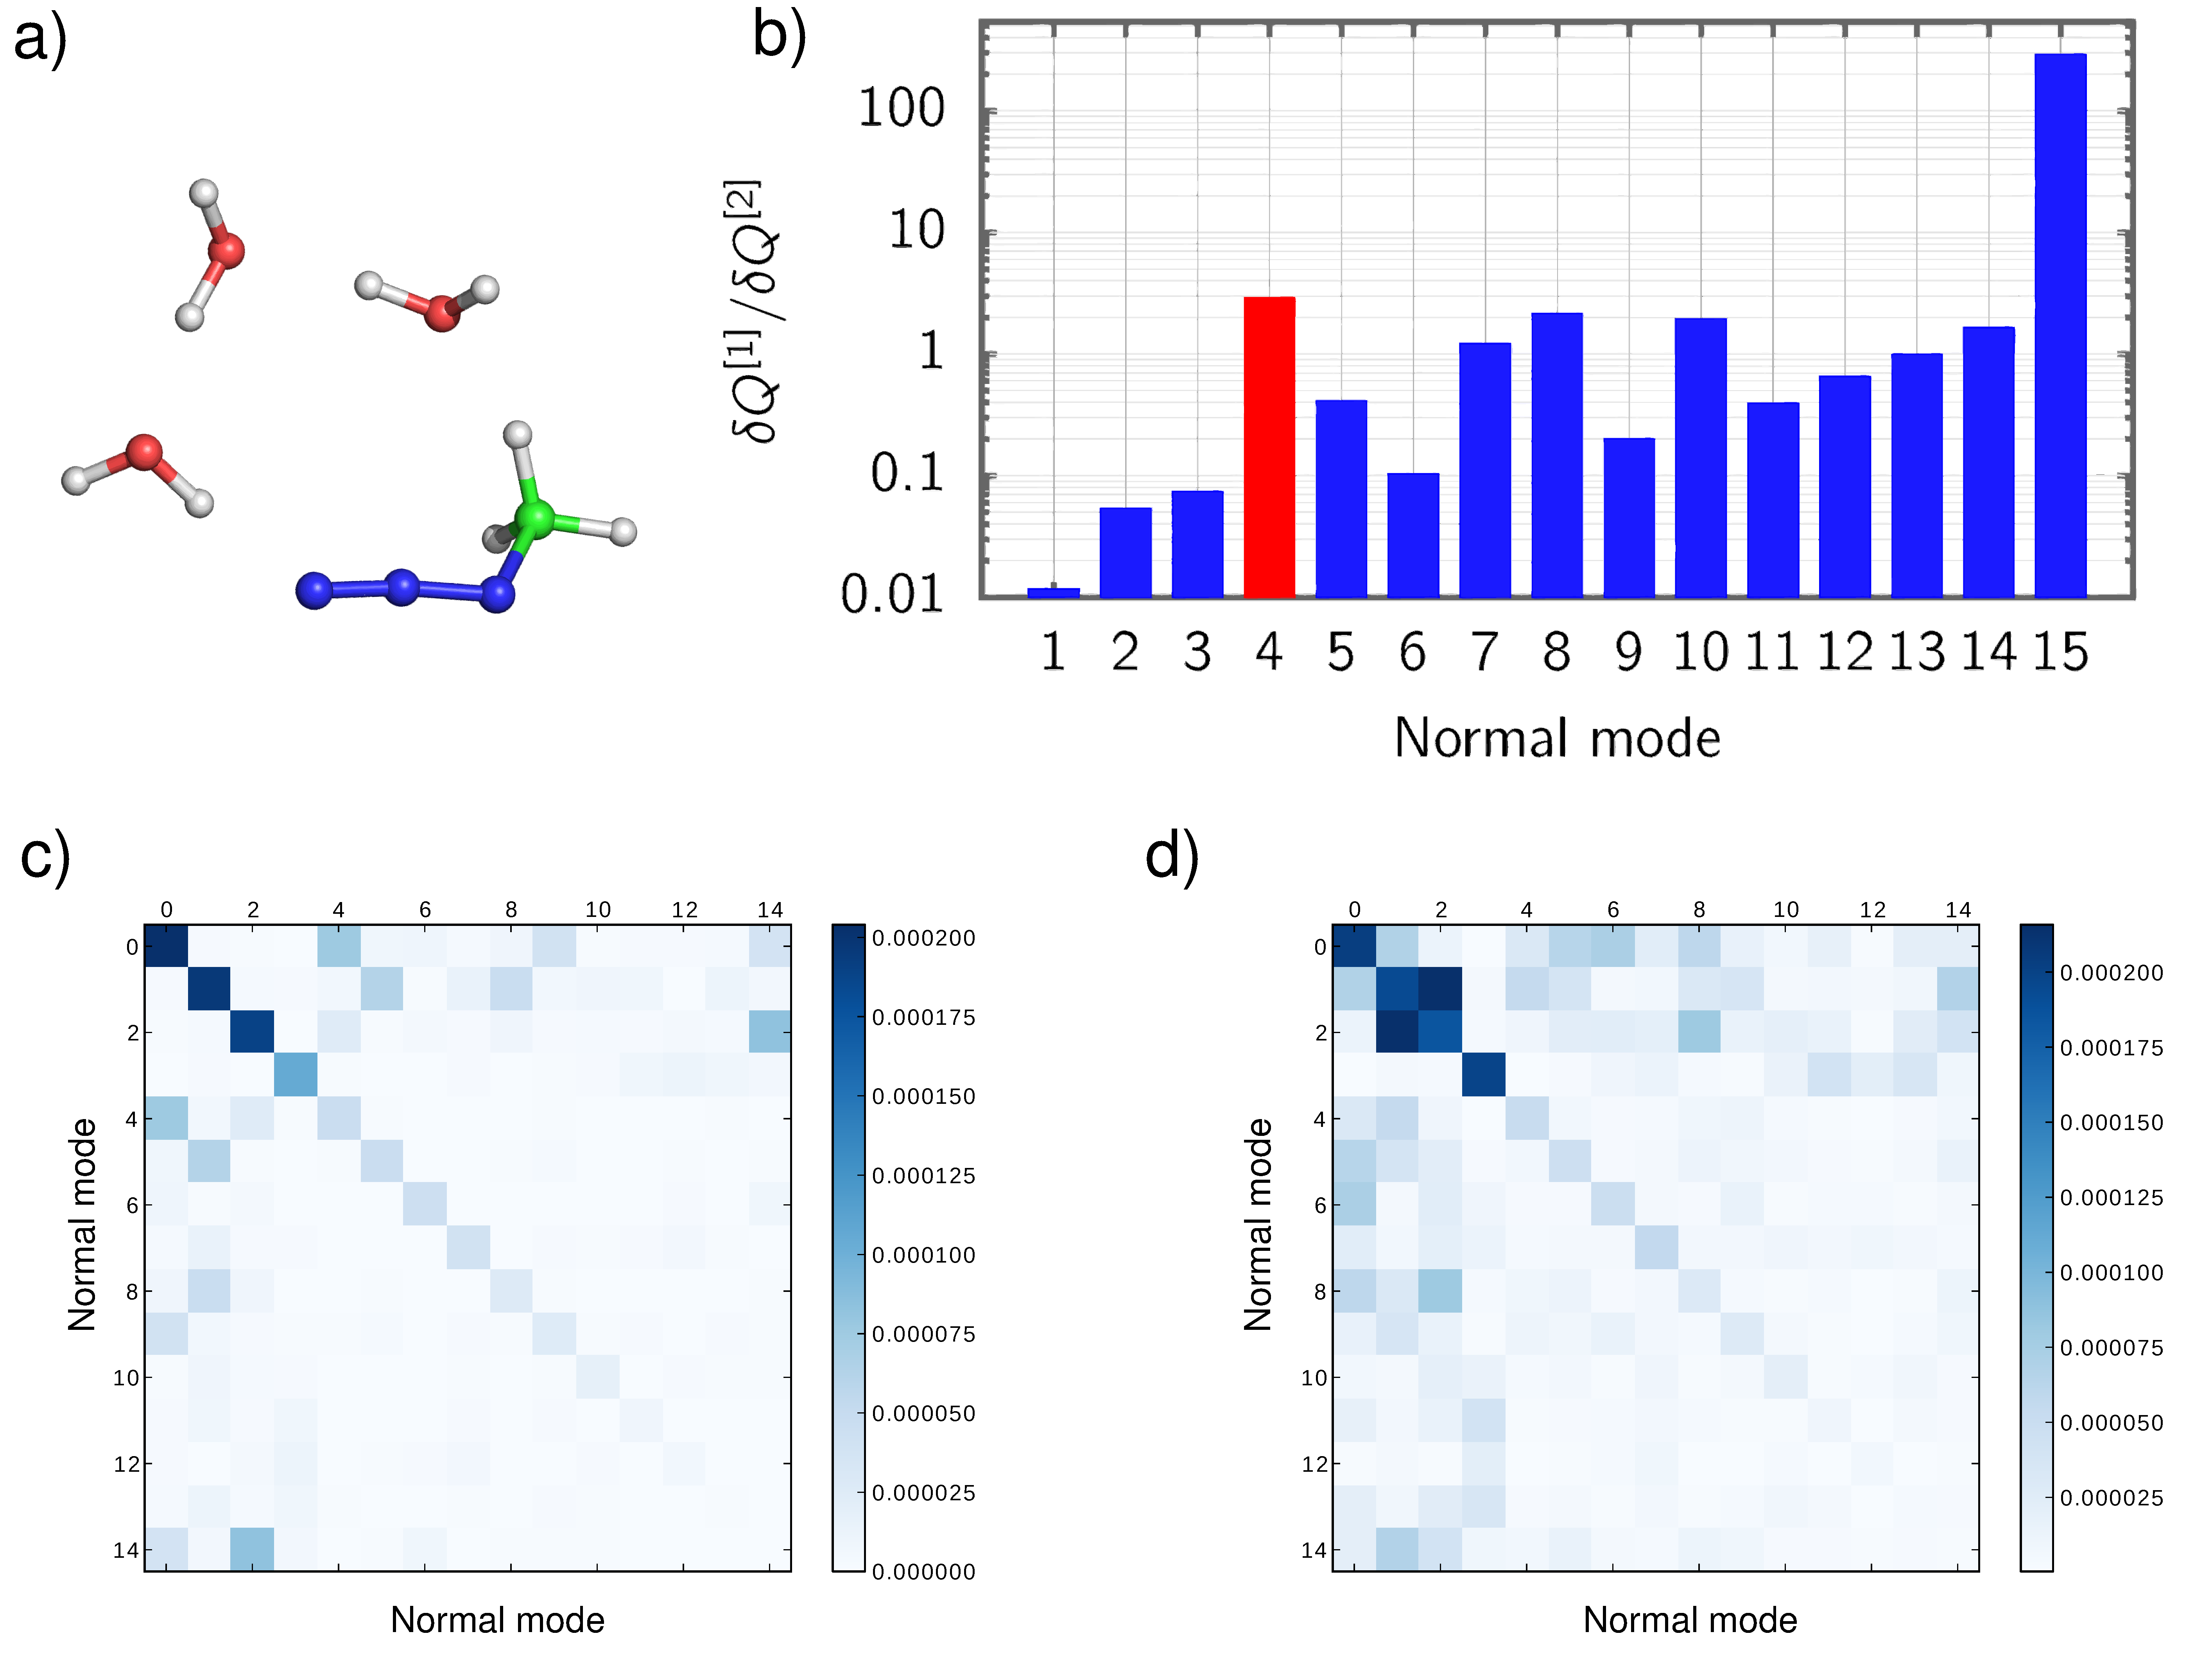
\includegraphics[width=0.9\linewidth]{Fig-men3-dq.eps}
}
\caption{Structural distortions of MeN$_3$ molecule and the resulting vibrational
frequencies calculated by using B3LYP/6-311++G(d,p) method. 
a) The structure of a model complex; b) relative differences of the
structural distortions
calculated for each normal mode displacement; c) and d) Hessian matrix in MeN$_3$ gas-phase normal coordinate
space calculated by using $\delta {\bf Q}^{[1]}$ and $\delta {\bf Q}^{[2]}$, respectively.
Hessian matrices were averaged over 20 model MeN$_3$--(H$_2$O)$_{n=1-10}$ configurations.
\label{f.MeN3.dq}}
\end{figure}
%

In fact, the differences in the vibrational solvatochromisms of NMA and MeN$_3$ are quite significant. 
This is because amide I modes are surprisingly well described by purely Coulombic 
models\citep{Blasiak.Lee.Cho.JCP.2013,Blasiak.Cho.JCP.2014,Blasiak.Cho.JCP.2015}
which is in stark contrast to triple\hyp{}bonded IR probes solvatochromisms such as 
CN, NC or N$_3$.\citep{Blasiak.Ritchie.Webb.Cho.XXX.2016,Blasiak.Maj.Cho.XXX.2016}
We will discuss this issue in more detail later when the non-Coulombic effects 
are also derived and extensively quantified.

In the examples studied above we considered the frequency of only localized 
normal modes. Nevertheless, when approximation '1'
is used, frequency shifts need to be computed under diagonal Hessian approximation
and it is not possible to study the intramolecular mode mixing process without additional 
modifications of the procedure. Therefore, approximation '2' might be useful when one
wanted to study the solvation\hyp{}induced mode mixing. Nevertheless, this aspect needs to
be investigated in more detail in the future.\footnote{The research presented here is not published yet.}
Moreover, electrostatic model is not working properly for azide IR probes.

\section{Vibrational Transition Dipole}

Up to that moment, we were considering only the vibrational frequency shifts
but it is also very useful to study the change of the vibrational
transition dipole due to solvation because it contains the critical
information about the changes in the IR absorption intensity.

To a good approximation, vibrational transition dipole is proportional to the dipole derivative 
with respect to the normal coordinate evaluated at the equilibrium geometry.
Therefore, it is sufficient to consider the change in the dipole derivative
upon solvation. In solution we have
%
\begin{equation} \label{e:dipole-solution}
{\BM \mu}({\bf F}) \approx {\BM \mu}_0 + {\BM \alpha}_0 \cdot {\bf F}
\end{equation}
%
and the dipole derivative is
%
\begin{equation} \label{e:dipole-der-solution}
 \frac{\partial{\BM \mu}({\bf F})}{\partial\overline{Q}_j} \Bigg|_{\overline{\bf Q}_{0_A}}
\approx 
 \frac{\partial{\BM \mu}({\bf F})}{\partial Q_j} \Bigg|_{{\bf Q}_{0_A}}
+
\sum_i \frac{\partial^2{\BM \mu}({\bf F})}{\partial Q_j \partial Q_i} \Bigg|_{{\bf Q}_{0_A}}
\left( \overline{Q}_i - Q_i\right)
\end{equation}
%
In the above equations, ${\BM \mu}_0$ and ${\BM \alpha}_0$ denote 
the solute's gas\hyp{}phase dipole moment
and polarizability, respectively.
Thus, by using the results obtained in Eqs.~\eqref{e:struct-dist-cho} 
and \eqref{e:struct-dist-cho-transl},
the difference transition dipole is given by
%
\begin{equation} \label{e:dipole-der-diff-solution}
\frac{\partial{\BM \mu}({\bf F})}{\partial\overline {\bf Q}_j} \Bigg|_{\overline{\bf Q}_{0_A}} -  
 \frac{\partial{\BM \mu}({\bf F}={\bf 0})}{\partial {\bf Q}_j} \Bigg|_{{\bf Q}_{0_A}} \approx
%
\frac{\partial{\BM \alpha}_0}{\partial Q_j} \Bigg|_{{\bf Q}_{0_A}} \cdot {\bf F}
+
\sum_i \frac{U_{0,i}}{M_i\omega_i^2} 
\left\{
\frac{\partial^2{\BM \alpha}_0}{\partial Q_j \partial Q_i} \Bigg|_{{\bf Q}_{0_A}} \cdot {\bf F}
+
\frac{\partial^2{\BM \mu}_0}{\partial Q_j \partial Q_i} \Bigg|_{{\bf Q}_{0_A}}
\right\}
\end{equation}
%
In a limiting case when
the interaction potential is approximated by the multipole expansion from
Eq.~\eqref{e:dmtp}, 
%and with constant $\nabla \phi$ 
%(i.e., $\phi({\bf r}) = {\bf r} \cdot {\bf F} + {\rm const.}$), 
Eq.~\eqref{e:dipole-der-diff-solution} can be recast 
in a simple form
%
\begin{equation} \label{e:dipole-der-diff-solution-field}
 \frac{\partial{\BM \mu}({\bf F})}{\partial\overline {\bf Q}_j} \Bigg|_{\overline{\bf Q}_{0_A}} -  
 \frac{\partial{\BM \mu}({\bf F}={\bf 0})}{\partial {\bf Q}_j} \Bigg|_{{\bf Q}_{0_A}} \cong
%
\left[
\frac{\partial {\BM \alpha}_0}{\partial Q_j} \Bigg|_{{\bf Q}_{0_A}} 
+ 
\sum_i \frac{1}{M_i\omega_i^2} 
\frac{\partial^2 {\BM \mu}_0}{\partial Q_j \partial Q_i} \Bigg|_{{\bf Q}_{0_A}}
\otimes
\frac{\partial {\BM \mu}_0}{\partial Q_i} \Bigg|_{{\bf Q}_{0_A}}
\right] 
\cdot {\bf F}
\end{equation}
%
in which we neglected the contributions of the polarizability second derivatives.

Note that the above discussion refers to the case
in which electric field is uniform in space. 
In the case when the electric field has a notable
gradients around the vibrational chromophore
the dipole\hyp{}dipole polarizability approximation from Eq.~\eqref{e:dipole-solution} 
is not sufficient. 

There are several ways to tackle the problem of non\hyp{}uniform
electric field.
One of them is to
add the quadrupole polarizabilities to Eq.~\eqref{e:dipole-solution} 
and obtain, for example, the contributions
of the kind $\frac{1}{3} \frac{\partial{\bf A}_0}{\partial Q_j} \big|_{{\bf Q}_{0_A}} \cdot {\BM \nabla}{\bf F}$ 
where ${\bf A}_0$ is the quadrupole-dipole polarizability. Another way is to use
charge\hyp{}response kernel approach in which
the first term in Eq.~\eqref{e:dipole-der-diff-solution} should be generalized 
to the following form\citep{Cho.JCP.2009}
%
\begin{equation} \label{e:trans-dip-cho-pot-ind-effect}
\left( \frac{\partial{\BM \alpha}_0}{\partial Q_j} \Bigg|_{{\bf Q}_{0_A}} \cdot {\bf F} \right)
\;\longrightarrow\;
2\int_V {\rm d}\;{\bf r} \int_V    {\rm d}\;{\bf r}' \; 
\left\{
\frac{\partial \kappa({\bf r},{\bf r}')}{\partial Q_j} \Bigg|_{{\bf Q}_{0_A}} {\bf r} \phi({\bf r}')
\right\}
%
\end{equation}
%
where $\kappa({\bf r},{\bf r}')$ denotes the charge response kernel
of solute. Analogously,
%
\begin{equation} \label{e:trans-dip-cho-pot-ind-effect-quadratic}
\left( \frac{\partial^2{\BM \alpha}_0}{\partial Q_j \partial Q_i} \Bigg|_{{\bf Q}_{0_A}} \cdot {\bf F} \right)
\;\longrightarrow\;
2\int_V {\rm d}\;{\bf r} \int_V    {\rm d}\;{\bf r}' \; 
\left\{
\frac{\partial^2 \kappa({\bf r},{\bf r}')}{\partial Q_j \partial Q_i} \Bigg|_{{\bf Q}_{0_A}} {\bf r} \phi({\bf r}')
\right\}
%
\end{equation}
%
Perhaps the most practical way is to employ the distributed
polarizabilities, i.e., do the replacement ${\BM \alpha}_0\rightarrow\sum_a{\BM \alpha}_{0,a}$
where the $a$th polarizable site is located at ${\bf r}_a$. 
In this scenario, the difference transition dipole 
is simply expressed as
%
\begin{multline}[box=\widebox] \label{e:dipole-der-diff-solution-distributed}
\frac{\partial{\BM \mu}({\bf F})}{\partial\overline {\bf Q}_j} \Bigg|_{\overline{\bf Q}_{0_A}} -  
 \frac{\partial{\BM \mu}({\bf F}={\bf 0})}{\partial {\bf Q}_j} \Bigg|_{{\bf Q}_{0_A}} \approx
%
\sum_a \left\{
\frac{\partial{\BM \alpha}_{a,0}}{\partial Q_j} \Bigg|_{{\bf Q}_{0_A}} 
+
\sum_i \frac{U_{0,i}}{M_i\omega_i^2} 
%
\frac{\partial^2{\BM \alpha}_{a,0}}{\partial Q_j \partial Q_i} \Bigg|_{{\bf Q}_{0_A}} 
\right\} \cdot {\bf F}({\bf r}_a) \\
+
\sum_i \frac{U_{0,i}}{M_i\omega_i^2}
\frac{\partial^2{\BM \mu}_0}{\partial Q_j \partial Q_i} \Bigg|_{{\bf Q}_{0_A}}
%
\qquad\qquad\qquad\qquad\qquad\qquad
\end{multline}
%
In the above expression, electric field is determined at
various polarizable sites which we denote here as ${\bf F}({\bf r}_a)$.

The theory presented in this Section is absolutely general 
for any kind of the solute\hyp{}solvent
interaction potential. Later on, we shall discuss the origins of the
vibrational frequency shifts and transition dipole differences
upon solvation.


\section{Summary}

In this Chapter, we have discussed the first\hyp{}principles
vibrational solvatochromism theories of Buckingham and Cho which,
although originate from different starting points, lead to the same results.
Thus, the vibrational solvatochromic frequency shift of a spatially localized 
IR probe normal mode can be described by Eq.~\eqref{e:buckingham-2st-order-total-fund}
which is second-order in the perturbation of the isolated harmonic oscillator Hamiltonian.
This model i) assumes the first\hyp{}order structural distortion of solute, which takes 
into account only the solute\hyp{}solvent interaction potential and neglects
solute's anharmonicity, as well as ii) considers the solvation\hyp{}induced change of the diagonal
Hessian matrix elements only. Therefore, we shall refer to this theory
as to the \emph{local mode approximation}. The theory reproduces well the frequency shifts of
simple localized vibrations as well as structural distortions
when the exact solute\hyp{}solvent interaction potential
is employed. However, since the local mode approximation cannot describe the normal modes
which are delocalized over many atoms, the approach of considering
the Hessian matrix proposed by Cho in Eq.~\eqref{e:force-const-cho} is necessary. 
In that case, particular caution should be made because the structural
distortion estimation is not well researched up to that moment. If the
first-order approximation from Eq.~\eqref{e:struct-dist-cho} failed in some cases, the results 
derived in Sec.~\ref{s:str-dist-general-discussion} might become useful.

\printbibliography[heading=subbibintoc,title={References}]
\end{refsection}

% === Chapter 4 ===
\begin{refsection}
\chapter{Origins of the Vibrational Solvatochromism \label{c:my-model}}

Although the theory of the vibrational solvatochromism
was developed before, it involved the solute\hyp{}solvent
intermolecular potential which is an extremely complicated function
of molecular properties.
Therefore, it is important to find explicit 
expressions that link the vibrational solvatochromism
to the particular interaction phenomenon.
Only then it is possible to obtain a robust model
that can be further applied for condensed phases. 
In this Chapter, we develop the rigorous first\hyp{}principles
theory of the vibrational frequency shifts and transition
dipole changes.
Due to historical reasons, we first develop a model in terms
of the implicit theories of solvation in which solute's molecular
environment is approximated by a continuum. 
Next, we derive the explicit theory based on five fundamental interactions
between molecules that can be found in nature: Coulombic, 
exchange\hyp{}repulsion, induction, dispersion and charge\hyp{}transfer.
Finally, we develop an approximate approach to
to estimating the long\hyp{}range corrections to the vibrational
frequency shifts when the solution extends to infinity.

\section{Implicit model: Coulombic and induction effects}

At the heart of the foundations of our knowledge about the 
physical chemistry of liquids and solutions are the \emph{continuum}
models of Onsager, Kirkwood and Fr{\"o}hlich. They
provided invaluable insight into the solvation
process from statistical thermodynamical point of view, linking
the microscopic characteristics of molecular species
with the macroscopic representatives of liquids
such as density, dielectric constant or refractive index.
Despite they cannot capture all the intermolecular
interactions effects rigorously, they do often provide a surprisingly 
correct
description of various observables in solution.
Therefore, it is instructive to study continuum models of solvation
in terms of the vibrational solvatochromism since they 
are still used by some researchers to relate macroscopic
solvent properties with molecular vibrational characteristics
in aprotic solvents.

As the simplest case let us consider the situation
in which the neutral solute molecule with the permanent gas\hyp{}phase 
dipole moment ${\BM \mu}_0$
is placed inside a spherical cavity of radius $a$, i.e., the 
Onsager model. 
%Note that
%for our purpose the cavity need to be quite large. Therefore 
%we can safely neglect other than dipole\hyp{}dipole interactions
%and consider the Onsager model of solvation.
In such a case, the solvation (interaction) energy is given as
%
\begin{equation} \label{e:esol-onsager}
 U^{\rm Sol}(\varepsilon, {\bf Q}) =
 -\frac{1}{2} {\BM \mu}(\varepsilon, {\bf Q}) \cdot {\bf F}^{\rm Ons}
\end{equation}
%
where the Onsager reaction (electric) field acting on the solute molecule
is
%
\begin{equation} \label{e:fons}
  {\bf F}^{\rm Ons} = \frac{2(\varepsilon-1)(n^2+1)}{3a^3(2\varepsilon+n^2)} {\BM \mu}(\varepsilon, {\bf Q})
 = g(a,\varepsilon) {\BM \mu}(\varepsilon, {\bf Q})
\end{equation}
%
In the above equations, ${\BM \mu}(\varepsilon, {\bf Q})$ 
is the total solute's (gas\hyp{}phase and induced) dipole moment.
It is strighforward to write down the expression for the
vibrational frequency shift as
%
\begin{equation} \label{e:dw-ons-gen}
  \Delta\omega_j(\varepsilon, {\bf Q}) = \hat{F}_j \left[ U^{\rm Sol}(\varepsilon, {\bf Q}) \right]
\end{equation}
%
where $\hat{F}_j$ is the vibrational solvatochromic frequency shift 
operator from Eq.~\eqref{e:dw-fea-fma}.

To calculate the solvatochromic vibrational frequency shift
using solute's gas\hyp{}phase properties it is necessary to expand
the dipole moment into a power series with respect to the two perturbations,
i.e., structural distortion and the Onsager electric field. Considering the first
four terms in the Taylor expansion of ${\BM \mu}(\varepsilon, {\bf Q})$ one gets
%
\begin{equation} \label{e:mu-qf}
 {\BM \mu}(\varepsilon, {\bf Q}) \approx 
 {\BM \mu}_0 + \fderiv{{\BM \mu}}{\bf F}\Bigg|_{0}  \cdot {\bf F}^{\rm Ons}
 + \sum_i \fderiv{{\BM \mu}}{Q_i}\Bigg|_{0} \delta Q_i 
 + \sum_i \sderivd{{\BM \mu}}{{\bf F}}{Q_i}\Bigg|_{0} \cdot {\bf F}^{\rm Ons} \delta Q_i
\end{equation}
%
where the subscript $0$ denotes that the derivatives are evaluated in the gas phase,
i.e., ${\bf F}={\bf 0}$ and $\delta Q_i=0$. Computation of the solute dipole
moment is not so easy since the relaxation process of the electronic wavefunction
and molecular structure has to be taken into account. This can 
be introduced in a one\hyp{}electron Hamiltonian in the Schr{\"o}dinger equation
or its approximate form. However, this is still relatively costly. Beneath
we present the approximate method of taking into account
this relaxation process basing solely on the solute's gas\hyp{}phase properties.

\subsection{Rigid molecule approximation}

Let us first consider the case when we neglect structural
relaxation due to the reaction field and focus only
on the electronic charge density redistribution. In such a case,
%
\begin{equation}
 {\BM \mu}(\varepsilon, {\bf Q}) \approx 
 {\BM \mu}_0 + {\BM \alpha}_0  \cdot {\bf F}^{\rm Ons}
\end{equation}
%
where the dipole\hyp{}dipole gas\hyp{}phase polarizability is
%
\begin{equation}
{\BM \alpha}_0  = \fderiv{{\BM \mu}}{\bf F}\Bigg|_{0}
\end{equation}
%
Then, the Onsager reaction field can be approximately written as
%
\begin{equation}
{\bf F}^{\rm Ons} \approx g(a,\varepsilon) {\bf B} \cdot {\BM \mu}_0
\end{equation}
%
with the auxiliary matrix given as follows
%
\begin{equation}
{\bf B} = \left( \mathbb{1} - g(a,\varepsilon){\BM \alpha}_0 \right)^{-1}
\end{equation}
%
Thus, the resulting solvation energy can be recast in the form
that depends only on gas\hyp{}phase solute properties:
%
\begin{equation} \label{e:ons-e-sol-init}
U^{\rm Sol}(\varepsilon, \delta{\bf Q}=0) = -\frac{1}{2} {\BM \Phi}(a, \varepsilon) : {\BM \mu}_0 \otimes {\BM \mu}_0
\end{equation}
%
where the ${\BM \Phi}(a, \varepsilon)$ tensor is defined as
%
\begin{equation}
{\BM \Phi}(a, \varepsilon) = g(a,\varepsilon) {\bf B} + g^2(a,\varepsilon) {\bf B} {\BM \alpha}_0 {\bf B}
\end{equation}
%
Now, applying the vibrational solvatochromic frequency shift
operator to this solvation energy,
we find that the frequecy shift is
%
\begin{equation} \label{e:dw-ons-working-form}
\Delta\omega_j(\varepsilon, \delta{\bf Q}=0) = \frac{1}{4M_j\omega_j}
\left\{ \sum_i \frac{g_{ijj}}{M_i\omega_i^2}S_i - K_j \right\}
\end{equation}
%
where the coefficients are given as
%
\begin{subequations}
 \begin{align}
  S_i &= \fderiv{{\BM \Phi}}{Q_i} : {\BM \mu}_0 \otimes {\BM \mu}_0 
           + 2{\BM \Phi} : \fderiv{{\BM \mu}_0}{Q_i} \otimes {\BM \mu}_0 \label{e:ons-si-init}\\
  K_j &= \sderiv{{\BM \Phi}}{Q_j} : {\BM \mu}_0 \otimes {\BM \mu}_0
           + 2{\BM \Phi} : \left[ \sderiv{{\BM \mu}_0}{Q_j} \otimes {\BM \mu}_0 
           +  \fderiv{{\BM \mu}_0}{Q_j} \otimes \fderiv{{\BM \mu}_0}{Q_j} \right] 
           + 4\fderiv{{\BM \Phi}}{Q_j} : \fderiv{{\BM \mu}_0}{Q_j} \otimes {\BM \mu}_0  \label{e:ons-ki-init}
 \end{align}
\end{subequations}
%
Note that ${\BM \Phi}$ is symmetric.  

\subsection{Structural distortion effect: Iterative method}

Now, using Eq.~\eqref{e:struct-dist-cho}
we can estimate the structural distortion due to relaxation 
in the first approximation as
%
\begin{equation} \label{e:ons-dq-init}
\delta Q_i \approx \frac{S_i}{2M_i\omega_i^2}
\end{equation}
%
Thus, it becomes possible to iteratively take into account 
the structural distortion effects for the solute's permanent
dipole moment evaluation, which directly influences the 
frequency shift via Eqs.~\eqref{e:esol-onsager}, 
\eqref{e:dw-ons-gen} and \eqref{e:mu-qf}.

When $\hat{F}_j$ acts on the full solvation energy 
the vibrational frequency shift has the same form as 
in Eq.~\eqref{e:dw-ons-working-form}
but the $S_i$ and $K_j$ coefficients are now different:
%
\begin{subequations}
 \begin{align}
  S_i &= \fderiv{{\BM \mu}(\varepsilon,{\bf Q})}{Q_i} \cdot {\bf F}^{\rm Ons}
           + {\BM \mu}(\varepsilon,{\bf Q}) \cdot \fderiv{{\bf F}^{\rm Ons}}{Q_i}
        \label{e:ons-si-iter}  \\
  K_j &= 2\left[ 
             \sderiv{{\BM \mu}_0}{Q_j}  
        + 2 \fderiv{{\BM \alpha}_0}{Q_j}  \cdot \fderiv{{\bf F}^{\rm Ons}}{Q_j}
         \right] \cdot {\bf F}^{\rm Ons}
         + 4\fderiv{{\BM \mu}(\varepsilon,{\bf Q})}{Q_j} \cdot \fderiv{{\bf F}^{\rm Ons}}{Q_j}
        \label{e:ons-ki-iter}
 \end{align} % i have multiplied K_j by 2
\end{subequations}
%
Analogously, the structural distortion is 
$\delta Q_i=S_i/2M_i\omega_i^2$.
One of the necessary derivatives are directly found to be
%
\begin{multline} \label{e:mu-qf-derivative}
\fderiv{{\BM \mu}(\varepsilon,{\bf Q})}{Q_j} =
\fderiv{{\BM \mu}_0}{Q_j} + \fderiv{{\BM \alpha}_0}{Q_j}  \cdot {\bf F}^{\rm Ons}
+ \sum_i \sderivd{{\BM \mu}_0}{Q_j}{Q_i} \delta Q_i 
+ \sum_i \sderivd{{\BM \alpha}_0}{Q_j}{Q_i} \cdot {\bf F}^{\rm Ons} \delta Q_i \\
+ {\BM \alpha}_0  \cdot \fderiv{{\bf F}^{\rm Ons}}{Q_j} 
+ \sum_i \fderiv{{\BM \alpha}_0}{Q_i} \delta Q_i \cdot \fderiv{{\bf F}^{\rm Ons}}{Q_j} 
\end{multline}
%
Moreover, from Eqs.~\eqref{e:mu-qf}
and \eqref{e:fons} one can easily find that
the Onsager reaction field is given as
%
\begin{equation} \label{e:ons-field}
 {\bf F}^{\rm Ons} = -{\bf A}^{-1} \cdot 
\left[ 
   {\BM \mu}_0 + \sum_i \fderiv{{\BM \mu}_0}{Q_i}\delta Q_i
\right]
\end{equation}
%
where the matrix $\bf A$, which can be viewed as generalized polarizability,
is
%
\begin{equation} \label{e:a-matrix}
{\bf A} = {\BM \alpha}_0 - \frac{1}{g(a,\varepsilon)} \mathbb{1} 
   + \sum_i \fderiv{{\BM \alpha}_0}{Q_i}\delta Q_i
\end{equation}
%
Thus the derivatives of the Onsager field are found to be
%
\begin{equation} \label{e:ons-field-deriv}
\fderiv{{\bf F}^{\rm Ons}}{Q_j}  = 
- {\bf A}^{-1} 
   \left[ 
       \fderiv{{\BM \mu}_0}{Q_j} 
      + \sum_i \sderivd{{\BM \mu}_0}{Q_j}{Q_i} \delta Q_i 
      - \fderiv{{\bf A}}{Q_j}  {\bf A}^{-1}  
           \left\{ 
               {\BM \mu}_0 + \sum_i \fderiv{{\BM \mu}_0}{Q_i}\delta Q_i
           \right\}
   \right]
\end{equation}
%
where
%
\begin{equation}
  \fderiv{{\bf A}}{Q_j} = \fderiv{{\BM \alpha}_0}{Q_j} 
               + \sum_i \sderivd{{\BM \alpha}_0}{Q_j}{Q_i}
\end{equation}
%
We are now ready to outline the iterative procedure
to converge $U^{\rm Sol}$ with respect to both electronic
charge density polarization and the structural
relaxation:
%
\begin{itemize}
\item[\textbullet] {\bf Initial Conditions}. 
                        By starting from rigid molecule approximation,
                        precompute the solvation energy from Eq.~\eqref{e:ons-e-sol-init}
                        and the initial structural distortions
                        from Eq.~\eqref{e:ons-dq-init} and 
                        Eq.~\eqref{e:ons-si-init}
\item[\textbullet] {\bf Iterations}. Start the iterative procedure 
                        by recomputing $U^{\rm Sol}$ and $\delta Q_i$
\begin{enumerate}
 \item Calculate Onsager field using Eqs.~\eqref{e:ons-field} and \eqref{e:a-matrix}, 
       and its derivatives from Eq.~\eqref{e:ons-field-deriv}
 \item Calculate dipole moment using Eq.~\eqref{e:mu-qf} 
       and its derivatives from Eq.~\eqref{e:mu-qf-derivative}
 \item Calculate structural distortions from Eq.~\eqref{e:ons-dq-init}
       and Eq.~\eqref{e:ons-si-iter}
 \item Calculate solvation energy using Eq.~\eqref{e:esol-onsager}
 \begin{itemize}
      \item if $\left| U^{\rm Sol}_{\rm old} - U^{\rm Sol}_{\rm new}\right| > \Delta U^{\rm crit}$:
            continue by updating the derivatives of dipole moment and Onsager field
            and going back to the next iteration
      \item else: End. 
 \end{itemize}    
\end{enumerate}
\end{itemize}
%
Once the solvation energy is converged 
(lowered as solute molecule
relaxes from its gas\hyp{}phase geometry) 
up to a chosen criterion $\Delta U^{\rm crit}$
one can readily obtain
the vibrational frequency shift by using Eqs.~\eqref{e:dw-ons-working-form},
\eqref{e:ons-si-iter} and \eqref{e:ons-ki-iter}.

In terms of accuracy, the rigid molecule approximation
provides already a good solvation energies and the frequency shifts
even for small cavity sizes which are simulating the molecular
volume
(see Chapter X). 
%Therefore, to estimate
%the frequency shift long\hyp{}range correction
%it is sufficient to focus
%on the approximation given in Eq.~\eqref{e:ons-e-sol-init}
%and the resulting vibrational frequency shift.
%This is mostly because, for our purposes, $a$ shall be typically
%large (much larger than the effective radius of the molecular
%charge distribution), and the structural distortion effects can be 
%neglected without significant loss of accuracy.

\subsection{The nature of interactions in Onsager model}

Onsager solvation energy is derived based on solving Poisson
equation for the boundary conditions specified by a point
dipole in a cavity surrounded by continuum dielectric.
Therefore the electrostatic effects that include polarization
energy are treated semi\hyp{}classically.

Let us study the origin of the vibrational frequency shift
within the Onsager model. 
%To obtain the explicit forms of $\Delta\omega_j^{\rm Coul}$
%and $\Delta\omega_j^{\rm Ind}$
%$\widetilde{\Delta\omega}_j^{\rm Coul}$
%and $\widetilde{\Delta\omega}_j^{\rm Ind}$ 
When the structural relaxation effect on solute's dipole moment
is neglected we can rewrite the frequency shift to be
%
\begin{multline} \label{e:f9f9f}
 \Delta\omega_j(\varepsilon, a) = 
- \left[ {\BM \mu}_j + \frac{1}{2} {\BM \mu}_j^{\rm Ind} \right] \cdot {\bf F}^{\rm Ons} 
- \frac{1}{2} {\BM \alpha}_j : {\bf F}^{\rm Ons} \otimes {\bf F}^{\rm Ons} 
+ \widetilde{\Delta\omega}_j({\bf F})
\\ = \Delta\omega_j^{\rm Coul} + \Delta\omega_j^{\rm Ind}
\end{multline}
%
where the Coulombic and induction frequency shifts 
are defined as
%
\begin{subequations}
 \begin{align}
   \Delta\omega_j^{\rm Coul}             &= - {\BM \mu}_j \cdot {\bf F}^{\rm Ons} + \Delta\omega_j({\bf F})\\
   \Delta\omega_j^{\rm Ind}              &= - \frac{1}{2} {\BM \mu}_j^{\rm Ind} \cdot {\bf F}^{\rm Ons} 
       - \frac{1}{2} {\BM \alpha}_j : {\bf F}^{\rm Ons} \otimes {\bf F}^{\rm Ons} 
 \end{align}
\end{subequations}
%
The effective gas\hyp{}phase and induced solvatochromic dipoles
are defined as
%
\begin{subequations}
 \begin{align}
   {\BM \mu}_j &= \frac{1}{2M_j\omega_j}
\left[  \sderiv{{\BM\mu}_0}{Q_j}
- \sum_i \frac{g_{ijj}}{M_i\omega_i^2} \fderiv{{\BM\mu}_0}{Q_i}
\right] \\
   {\BM \mu}_j^{\rm Ind} &= \frac{1}{2M_j\omega_j} 
\left[ 8 \fderiv{{\bf F}^{\rm Ons}}{Q_j} \cdot \fderiv{{\BM\alpha}_0}{Q_j} - 
   \sum_i \frac{g_{ijj}}{M_i\omega_i^2} \fderiv{{\bf F}^{\rm Ons}}{Q_i} \cdot {\BM\alpha}_0
\right]
 \end{align}
\end{subequations}
%
whereas the solvatochromic polarizability is
%
\begin{equation} 
  {\BM \alpha}_j = - \frac{1}{2M_j\omega_j} 
   \sum_i \frac{g_{ijj}}{M_i\omega_i^2} \fderiv{{\BM\alpha}_0}{Q_i}
\end{equation}
%
In Eq.~\eqref{e:f9f9f}, we separated the 'electric-field correction'
term from the Coulombic term due to technical reasons,
%
\begin{equation} 
\Delta\omega_j({\bf F}) = \frac{1}{4M_j\omega_j}
\sum_i \frac{g_{ijj}}{M_i\omega_i^2} \left\{ {\BM\mu}_0 + 
2\delta_{ij}\frac{M_i\omega_i^2}{g_{ijj}}\fderiv{{\BM\mu}_0}{Q_i}\right\} \cdot \fderiv{{\bf F}^{\rm Ons}}{Q_i}
\end{equation}
%
This contribution depends on the electric field changes along the vibrational
coordinate while it does not involve the polarizability. Therefore
it cannot be written in a way that is analogous
to the conventional multipole expansion of interaction energy 
in which dipoles (permanent and induced) interact with electric fields.

As can be seen, Onsager model includes semiclassically
Coulombic and induction energies. However, it cannot
deal with dispersion effects that are fully quantum mechanical
in nature. Moreover,
%It is interesting to note the straightforward
%similarity of the above equations to the corresponding
%contributions in the descrete model of vibrational
%solvatochromism discussed in previous Sections.
Onsager model (and any other continuum approach) 
is incapable of modelling
explicit solvation effects such as molecular collisions
and specific interactions. Therefore, its significance
lies mostly in the concept of the non\hyp{}specific
vibrational frequency shift (due to electrostatic
interactions) and should not be used for quantitative
calculations, especially when specific interactions such as
hydrogen bonds are present solute and its molecular environment.



\section{Coulombic Effects\label{s:dw-coul}}

In the first\hyp{}order of polarization perturbation
theory\footnote{i.e., in the long\hyp{}distance limit 
where the wavefunction overlap vanishes. In such a case the
exchange and charge\hyp{}penetration effects 
between solute and solvent molecules can be safely ignored.}, 
the intermolecular interaction potential
can be understood as a Coulombic interaction
of unperturbed solute and solvent molecules (i.e., 
as if they were isolated).\citep{Jeziorski.Moszynski.Szalewicz.ChemRev.1994,Stone.TheTheoryOfIntermolecularForces.1996}
That is
%
\begin{equation} \label{e:eint-1}
U^{(1)} = 
\langle 0_A0_B \lvert \mathscr{V}_{AB} \rvert 0_A0_B \rangle 
\end{equation}
%
Here, $\mathscr{V}_{AB}$ is the solute\hyp{}solvent
interaction potential defined as $\mathscr{V}_{AB}\equiv\mathscr{H}_{AB} - \mathscr{H}_{0_A} - \mathscr{H}_{0_B} $,
and $\vert 0_A0_B \rangle \cong \vert 0_A \rangle \otimes \vert 0_B \rangle$
and $\vert mn \rangle \cong \vert m \rangle \otimes \vert n \rangle$
represent the electronic ground state and excited states
of the $AB$ complex, respectively. The isolated electronic states of monomers $A$
and $B$ are determined by the time\hyp{}independent Schr{\"o}dinger
equations
%
\begin{subequations}
 \begin{align}
  \mathscr{H}_{0_A} \vert m \rangle &= \hbar \omega_m \vert m \rangle \\
  \mathscr{H}_{0_B} \vert n \rangle &= \hbar \omega_n \vert n \rangle
 \end{align}
\end{subequations}
%
Then it becomes legitimate to model the electrostatic interaction
energy by considering the distributed multipole expansion of electron
charge density distributions\citep{Stone.TheTheoryOfIntermolecularForces.1996}
which is given in Eq.~\eqref{e:dmtp}. Analogously,
the electrostatic potential and its gradients
can be also multipole\hyp{}expanded as follows
%
\begin{equation} \label{e:potential-gradients}
\underbrace{\nabla \otimes \cdots \otimes \nabla}_{r} \phi({\bf r}_x) = 
\sum_y \left[ 
{\bf T}^{(r)} q_y - {\bf T}^{(r+1)} \cdot {\BM \upmu}_y + 
 \frac{1}{3} {\bf T}^{(r+2)} : {\BM \Theta}_y - 
\frac{1}{15} {\bf T}^{(r+3)} : {\BM \Omega}_y + \ldots
\right]
\end{equation}
%
where 
$\nabla \equiv \sum_{\zeta}^{x,y,z} \hat{\bf i}_\zeta \frac{\partial}{\partial \zeta_x}$, 
$y$ runs over all solvent electrostatic distributed sites
and ${\bf T}^{(r)}$ are the so called interaction tensors of rank $r$ which are defined as follows
%
\begin{subequations}
\label{e:interaction-tensors}
\begin{align}
  T^{(0)} &= \frac{1}{\rvert {\bf r}_{xy} \lvert}  \label{e:interaction-tensors-1} \\
  T^{(1)}_\alpha &=-\frac{{\bf r}_{xy;\alpha}}{\rvert {\bf r}_{xy} \lvert^3}  \label{e:interaction-tensors-2} \\
  T^{(2)}_{\alpha\beta} &=3\frac{{\bf r}_{xy;\alpha} {\bf r}_{xy;\beta} }{\rvert {\bf r}_{xy} \lvert^5}  
      - \frac{\delta_{\alpha\beta}}{\rvert {\bf r}_{xy} \lvert^3}             \label{e:interaction-tensors-3} \\
  T^{(3)}_{\alpha\beta\gamma} &= -15 
         \frac{{\bf r}_{xy;\alpha} {\bf r}_{xy;\beta} {\bf r}_{xy;\gamma} }{\rvert {\bf r}_{xy} \lvert^7}
                  +3 \frac{{\bf r}_{xy;\alpha} \delta_{\beta\gamma}+
                           {\bf r}_{xy;\beta}  \delta_{\alpha\gamma}+
                           {\bf r}_{xy;\gamma} \delta_{\alpha\beta}}{\rvert {\bf r}_{xy} \lvert^5} \label{e:interaction-tensors-4}
\end{align}
\end{subequations}
%
with ${\bf r}_{xy} \equiv {\bf r}_x - {\bf r}_y$.

The solvatochromic multipole series expansion given in Eq.~\eqref{e:dmtp-sol}
is approximate because it neglects the change of the electrostatic
potential when the vibration occurs. Here we re\hyp{}derive the 
expression for the frequency shift with explicit inclusion of derivatives
of $\phi$. The first and second derivatives of the Coulombic
electrostatic energy can be expressed as follows\citep{Blasiak.Cho.JCP.2014}:
%
\begin{multline} \label{x:726439}
 \fderiv{U^{\rm Coul}}{Q_i} =
%
\sum_x 
\Bigg[ 
  \fderiv{q_x}{Q_i} \phi({\bf r}_x) + 
  \fderiv{{\BM \upmu}_x}{Q_i} \cdot \nabla \phi({\bf r}_x) + \frac{1}{3}  
  \fderiv{{\BM \Theta}_x}{Q_i} : \nabla\nabla \phi({\bf r}_x) \\ + \frac{1}{15}   
  \fderiv{{\BM \Omega}_x}{Q_i} \vdots \nabla\nabla\nabla \phi({\bf r}_x) + \ldots 
\Bigg] 
%
+
%
\sum_x 
\Bigg[ 
  q_x \fderiv{\phi({\bf r}_x)}{Q_i} + 
  {\BM \upmu}_x \cdot \fderiv{\nabla \phi({\bf r}_x)}{Q_i} \\ + \frac{1}{3} 
  {\BM \Theta}_x : \fderiv{\nabla\nabla \phi({\bf r}_x)}{Q_i} + \frac{1}{15}
  {\BM \Omega}_x \vdots \fderiv{\nabla\nabla\nabla \phi({\bf r}_x)}{Q_i} + \ldots 
\Bigg]
\end{multline}
%
and
%
\begin{multline} \label{x:726440}
 \sderiv{U^{\rm Coul}}{Q_i} =
%
\sum_x 
\Bigg[ 
  \sderiv{q_x}{Q_i} \phi({\bf r}_x) + 
  \sderiv{{\BM \upmu}_x}{Q_i} \cdot \nabla \phi({\bf r}_x) + \frac{1}{3}  
  \sderiv{{\BM \Theta}_x}{Q_i} : \nabla\nabla \phi({\bf r}_x) \\ + \frac{1}{15}   
  \sderiv{{\BM \Omega}_x}{Q_i} \vdots \nabla\nabla\nabla \phi({\bf r}_x) + \ldots 
\Bigg] 
%
+
%
\sum_x 
\Bigg[ 
  q_x \sderiv{\phi({\bf r}_x)}{Q_i} + 
  {\BM \upmu}_x \cdot \sderiv{\nabla \phi({\bf r}_x)}{Q_i} \\ + \frac{1}{3} 
  {\BM \Theta}_x : \sderiv{\nabla\nabla \phi({\bf r}_x)}{Q_i} + \frac{1}{15}
  {\BM \Omega}_x \vdots \sderiv{\nabla\nabla\nabla \phi({\bf r}_x)}{Q_i} + \ldots 
\Bigg]
\end{multline}
%
where, for the sake of notational simplicity, 
it is assumed that the derivatives are to be evaluated at
solute's gas phase equilibrium geometry.

In the previous studies only the first summation terms in 
Eqs.~\eqref{x:726439} and \eqref{x:726440} were taken into account because 
they were assumed to be the dominant contributions. To evaluate the
magnitudes of all the other remaining terms, one has to calculate
the derivatives of electrostatic potential (and its spatial gradients)
with respect to the normal coordinate. Rewriting the differential 
operators and using the chain rule, we can simplify the
derivative operators in the following way
%
\begin{subequations}  \label{e:deriv-operators}
\begin{align}
\fderiv{}{Q_i} &= \sum_m \fderiv{r_m}{Q_i}\fderiv{}{r_m} 
     \approx \sum_{m\in x} \fderiv{r_m}{Q_i}\fderiv{}{r_m} 
     = {\bf L}_x^{(i)} \cdot {\BM \nabla}_x      \label{e:deriv-operators-1} \\
\sderiv{}{Q_i} &= \sum_{mn} \fderiv{r_m}{Q_i}\fderiv{r_n}{Q_i}\sderivd{}{r_m}{r_n} 
     \approx \sum_{m\in x}\sum_{n\in x} \fderiv{r_m}{Q_i}\fderiv{r_n}{Q_i}\sderivd{}{r_m}{r_n} 
     = {\bf L}_x^{(i)} \otimes {\bf L}_x^{(i)} : {\BM \nabla}_x{\BM \nabla}_x  \label{e:deriv-operators-2}
\end{align}
\end{subequations}
%
where $n$ and $m$ represent the Cartesian coordinatesof solute
atomic centers and ${\bf L}_x^{(i)}$ denotes the mass\hyp{}weighted
eigenvector referring to the motion of atom $x$ along $Q_i$
(see Appendix~\ref{asec:vibranal} for more details on how to obtain these vectors).
In the above derivations we assumed that the change of the electrostatic
potential due to the displacement alont the normal coordinate is, 
to a good approximation, local, that is to say, only the change of the
atomic position ${\bf r}_x$ is important for which electrostatic potential 
is evaluated. This is equivalent to neglecting the intramolecular induction
effects.

Inserting Eqs.~\eqref{e:deriv-operators-1} and ~\eqref{e:deriv-operators-2}
into Eqs.~\eqref{x:726439} and ~\eqref{x:726440} and properly 
grouping terms with the same characters, we obtain
the first and the second derivatives of the intermolecular interaction
potential, which are associated with each multipole moment, i.e.,
%
\begin{subequations}  \label{e:f-terms}
\begin{align}
 U_i^{(q)}          &= \sum_x 
  \left[ \fderiv{q_x}{Q_i} \phi({\bf r}_x) 
 + q_x {\bf L}_x^{(i)} \cdot \nabla \phi({\bf r}_x) \right]       
                                                                \label{e:f-terms-1} \\
 U_i^{(\BM\upmu)}     &= \sum_x  
  \left[ \fderiv{{\BM \upmu}_x}{Q_i} \cdot \nabla\phi({\bf r}_x) 
 + {\BM \upmu}_x \otimes {\bf L}_x^{(i)} : \nabla\nabla \phi({\bf r}_x) \right]     
                                                                \label{e:f-terms-2} \\
 U_i^{(\BM\Theta)}  &= \sum_x  
  \left[ \fderiv{{\BM \Theta}_x}{Q_i} : \nabla\nabla\phi({\bf r}_x) 
 + {\BM \Theta}_x \otimes {\bf L}_x^{(i)} : \nabla\nabla\nabla \phi({\bf r}_x) \right]      
                                                                \label{e:f-terms-3} \\
 U_i^{(\BM\Omega)}  &= \sum_x      
  \fderiv{{\BM \Omega}_x}{Q_i} \vdots \nabla\nabla\nabla\phi({\bf r}_x)  
                                                                \label{e:f-terms-4} 
\end{align}
\end{subequations}
%
and
%
\begin{subequations}  \label{e:k-terms}
\begin{align}
 U_{jj}^{(q)}          &= \sum_x   
    \left[ \sderiv{q_x}{Q_j} \phi({\bf r}_x) 
    + 2 \fderiv{q_x}{Q_j} {\bf L}_x^{(j)} \cdot \nabla \phi({\bf r}_x) 
    + q_x \nabla\nabla \phi({\bf r}_x) : {\bf L}_x^{(j)} \otimes {\bf L}_x^{(j)} \right]     \label{e:k-terms-1} \\
%
 U_{jj}^{(\BM\upmu)}     &= \sum_x  
    \left[ \sderiv{{\BM \upmu}_x}{Q_j} \phi({\bf r}_x) 
    + 2 \fderiv{{\BM \upmu}_x}{Q_j} \otimes {\bf L}_x^{(j)} : \nabla\nabla \phi({\bf r}_x) 
    + {\BM \upmu}_x \cdot \nabla\nabla\nabla \phi({\bf r}_x) \vdots {\bf L}_x^{(j)} \otimes {\bf L}_x^{(j)} \right]      
    \label{e:k-terms-2} \\
%
 U_{jj}^{(\BM\Theta)}  &= \frac{1}{15} \sum_x  
    \left[ \sderiv{{\BM \Theta}_x}{Q_j} \phi({\bf r}_x) 
    + 2 \fderiv{{\BM \Theta}_x}{Q_j} \otimes {\bf L}_x^{(j)} \vdots \nabla\nabla\nabla \phi({\bf r}_x)  \right]      
    \label{e:k-terms-3} \\
%
 U_{jj}^{(\BM\Omega)}  &= \frac{1}{3} \sum_x \sderiv{{\BM \Omega}_x}{Q_j} \phi({\bf r}_x)       \label{e:k-terms-4}
\end{align}
\end{subequations}
%
For clarity, only tensors whose rank is less than four are keept in the above summations.
The formulae in Eqs.~\eqref{e:f-terms} and \eqref{e:k-terms} look rather formidable,
especially due to the fact that the potentials and their 
gradients\footnote{in the current implementation up to third rank}
have to be computed from Eq.~\eqref{e:potential-gradients}
which is also a multipole expansion. Therefore,
the electrostatic\hyp{}potential\hyp{}corrected frequency shift
becomes
%
\begin{equation} \label{e:dw-solefp-coul}
\Delta \omega_j^{\rm Coul} = \Delta \omega_j^{\rm SolDMA} + \Delta\omega_j({\partial\phi}) 
\end{equation}
%
where $\Delta \omega_j^{\rm SolDMA}$ is equal to the distributed multipole analysis (DMA)
expansion approximating the Coulombic frequency shift given in Eq.~\eqref{e:dmtp-sol} whereas
%
\begin{equation} \label{e:dw-solefp-coul-correction}
\Delta\omega_j({\partial\phi})  = -\frac{1}{2M_j\omega_j}
\sum_{x \in A}\sum_{y \in B}
\Big[
\sum_i  \frac{g_{ijj}}{M_i\omega_i^2} \sum_{r^{-n} \textrm{ terms} } U_i^{xy} - \sum_{r^{-n} \textrm{ terms} } U_{jj}^{xy}
\Big]
\end{equation}
%
The resulting terms $U_i^{xy}$ and $U_{jj}^{xy}$ in Eq.~\eqref{e:dw-solefp-coul-correction}
have various asymptotic distance dependences (denoted above as $r^{-n}$
where $r$ is the distance between the distributed multipole centers).
The explicit formulae
that can be directly implemented into a computer code
are listed in Appendix~\ref{a:fk-terms} according to $n$. 
Note that only terms with $n\ge 2$ contribute (i.e., charge-dipole
like terms) because of the differentiation operator.

Before we move to analyze the non\hyp{}Coulombic frequency shifts, two cautionary remarks
on the Coulomb frequency shift correction from Eq.~\eqref{e:dw-solefp-coul-correction} should be made.
First, note that, while $\Delta \omega_j^{\rm SolDMA}$ can be computed from the
solvatochromic multipoles that can be stored in a generalized object
describing a molecule, $\Delta\omega_j({\partial\phi})$ requires 
additionally other quantities that cannot be incorporated
into the definition of the solvatochromic multipole due to the directional
terms coupling solute and solvent distances. Therefore,
the evaluation of the frequency shift including electrostatic potential
correction complicates the implementation (additionally, multipole moments
and their first derivatives with respect to all the normal coordinates need 
to be stored as well). However, it is mostly the case
that $\Delta\omega_j({\partial\phi})$ is much smaller than $\Delta \omega_j^{\rm SolDMA}$
so under certain circumstances the former contribution could be
neglected.

Second, because the multipole series expansion of the interaction energy
is in principle divergent, the derivative of such series
with respect to normal coordinate is divergent as well. Moreover, 
there is no theorem stating that such a series will have the same radius of convergence
than the conventional interaction energy expansion. In fact,
we have found, by comparing the $r^{-n}$ terms contributions to the frequency
shifts, that in some cases the series diverges already for 
$r^{-3}$ contributions. Therefore, for practical reasons, only
the first correction terms that have $r^{-2}$ asymptotic dependence
are recommended be taken into account. In this approximation,
the Coulombic frequency shift has the following form
%
\begin{equation} \label{e:dw-solefp-coul-working}
\Delta\omega_j^{\rm Coul} \cong \Delta\omega_j^{\rm SolDMA} + \frac{1}{2M_j\omega_j}
\sum_i \frac{g_{ijj}}{M_i\omega_i^2} \sum_{x \in A}\sum_{y \in B}
\left\{ q_x - 2\delta_{ij} \fderiv{q_y}{Q_i} \right\} \frac{q_y}{r_{xy}^3} {\bf L}_x^{(i)} \cdot {\bf r}_{xy} 
\end{equation}
%
For the more detailed analysis of the convergence properties
of $\Delta\omega_j({\partial\phi})$ for some examplary model 
systems the Reader is reffered to
the Appendix~\ref{a:convergence-of-the-correction-terms}


\section{Polarization and dispersion effects}

In Section~\ref{s:dw-coul} we have focused on a long\hyp{}range
approximation of the electrostatic contribution to the frequency
shift that assumed that interacting species do not perturb
their charge densities. However, according to classical electrostatics,
it is well known that any charge density induces the new
charge density of opposite sign in a surrounding medium. In quantum
physics, this is manifested by induction effects due to the polarization
of the electronic density distribution of atoms. This causes
an additional attractive forces between molecules which
become stonger when the density distributions become more polarized
(e.g., dipole moment is large). Therefore, the
phenomenon of the \emph{induction} (or \emph{polarization}) effects
in the vibrational solvatochromism cannot be ignored.

In addition to polarization effects which can be treated
by semi\hyp{}classical theory, there is also yet another effect
which cannot be explained by classical physics. Due to the Heisenberg
uncertainty principle, the permanent multipole moments of the 
molecular charge distribution cannot be determined at an instant
of time within 100\% precision. There is always some uncertainty
in the multipole moment which leads to the additional stabilization
of the total energy of the system due to \emph{electron correlation}. This effect is
called \emph{dispersion} and plays very important role in chemistry.
This is the dispersion interactions which makes the neutral rare gas atoms 
like He or Ne
to attract each other with the strength of such attraction decreasing
with $r^{-6}$ where $r$ is the interatomic distance.

According to the polarization perturbation theory, the induction
and dispersion forces arise in the second\hyp{}order with respect to
the interaction 
operator.\citep{Stone.TheTheoryOfIntermolecularForces.1996,
Jeziorski.Moszynski.Szalewicz.ChemRev.1994} 
Thus, the second order correction to the total
energy of the system can be written as
%
\begin{equation} \label{e:eint-2}
U^{(2)} = - \sum_{mn\ne 00} \frac{
\langle 0_A0_B \lvert \mathscr{V}_{AB} \rvert mn \rangle \langle  mn \lvert \mathscr{V}_{AB} \rvert 0_A0_B \rangle
}{\hbar \left( \omega_{m0_A} + \omega_{n0_B}\right)}
\end{equation}
%

\subsection{Induction effects}

If we restrict the summation in Eq.~\eqref{e:eint-2} to run over such states
that involve ground state of either monomer
we get the second\hyp{}order induction energy. Mainly,
%
\begin{equation} \label{e:eint-2-ind}
U^{\rm Ind} = U^{\rm Ind}_A + U^{\rm Ind}_B =
- \sum_{m\ne 0} \frac{
\lvert \langle 0_A0_B \lvert \mathscr{V}_{AB} \rvert m0_B \rangle \rvert^2
}{\hbar \left( \omega_{m} - \omega_{0_A}\right)}
%
- \sum_{n\ne 0} \frac{
\lvert \langle 0_A0_B \lvert \mathscr{V}_{AB} \rvert 0_An \rangle \rvert^2
}{\hbar \left( \omega_{n} - \omega_{0_B}\right)}
\end{equation}
%
%The induction energy
%arises as a part of the second\hyp{}order 
Interaction potential can be then multipole\hyp{}expanded and
it can be shown that the induction energy
can be expressed as
%
\begin{equation} \label{e:eint-2-ind-mult}
U^{\rm Ind} = - \frac{1}{2} {\BM \alpha}_A : {\bf F} \otimes {\bf F} 
              - \frac{1}{2} {\BM \alpha}_B : {\bf F} \otimes {\bf F} + \ldots
\end{equation}
% 
where the ground\hyp{}state polarizability is defined as
%
\begin{equation} \label{e:polarizability}
{\BM \upalpha}_A = 2\sum_{m\neq 0} \frac{
\langle 0_A \lvert \hat{\BM \mu} \rvert m \rangle \otimes \langle m \lvert \hat{\BM \mu} \rvert 0_A \rangle 
}{\hbar \left( \omega_{m} - \omega_{0_A}\right)}
\end{equation}
%
and similarly for solvent molecule.\footnote{We emphasize here
that electric field $\bf F$ in the above expression
is the sum of the electric field produced by the permanent
multipole moments and the induced electric fields.}
It is more desirable to work with
the distributed polarizability picture because the series in 
Eq.~\eqref{e:eint-2-ind-mult} gives typically poor estimates of $U^{\rm Ind}$,
especially when dipole\hyp{}dipole approximation is invoked. 

According to Li \emph{et al.},\citep{Li.Netzloff.Gordon.JCP.2006} 
the induction interaction energy in the 
\emph{distributed} dipole\hyp{}dipole polarizability approximation 
can be written in the following form:
%
\begin{equation} \label{e:eint-2-ind-dip-distr}
U^{\rm Ind} = - \frac{1}{2} {\bf p} \cdot {\bf F} = - \frac{1}{2} {\bf F}^T \cdot {\bf D}^{-1} \cdot {\bf F}
\end{equation}
%
where ${\bf p}$ constitutes the induced dipoles of 
polarizable centers and ${\bf F}$ constitutes the electric field 
vectors evaluated at each polarizable center, which are created by the 
distributed static multipole moments of interacting molecules.
Mainly,
%
\begin{subequations} \label{e:pf}
\begin{align}
 {\bf p} &= 
 \begin{Bmatrix}
  {\bf p}_1 & {\bf p}_2 & \cdots & {\bf p}_N
 \end{Bmatrix} \\
 {\bf F}&= 
 \begin{Bmatrix}
  {\bf F}_1 & {\bf F}_2 & \cdots & {\bf F}_N
 \end{Bmatrix}
\end{align}
\end{subequations}
%
Thus, the length of these two vectors is $3N$ in contrast to the dimension
of $\bf F$ in Eq.~\eqref{e:eint-2-ind-mult} which is just the limitting case of 
Eq.~\eqref{e:eint-2-ind-dip-distr} with $N=1$.
The $\bf D$ matrix elements are defined as
%
\begin{equation} \label{e:D-matrix}
{\bf D}_{ab} = 
\left\{\begin{matrix}               
{\BM \alpha}_a^{-1} \delta_{ab} && \text{if $a$,$b$ belong to the same molecule} \\
-{\bf T}_{ab}^{(2)}             && \text{if $a$,$b$ belong to different molecules}
\end{matrix}\right. 
\end{equation}
%
where ${\BM \alpha}_a$ is the distributed state anisotropic polarizability
tensor. They can be calculated by using coupled\hyp{}perturbed Hartree\hyp{}Fock
theory by analyzing the response of the localized molecular orbitals
(LMO's) on the electric field perturbation. Note that the formalism
in Eq.~\eqref{e:eint-2-ind-dip-distr} uses a trick which enables one
to work with the \emph{static} (not induced) electric field while still taking
into account the induced electric fields in an exact manner. In fact,
the induced electric fields are taken into account in $\bf D$ matrix already
by the dipole\hyp{}dipole interaction tensors ${\bf T}_{ab}^{(2)}$.
Therefore, the inverse of $\bf D$ matrix generalizes
the polarizability for the $N$-body system in a special way, making use
of only permanent multipoles and polarizabilities which greatly simplifies
the computations.\footnote{Otherwise, electric fields must be iteratively converged to
self\hyp{}consistency.}

Now, the vibrational frequency shift due to induction can be written
as
%
\begin{equation}\label{e:dw-ind-base}
\Delta \omega_j^{\rm Ind} =
\frac{1}{2M_j\omega_j} \left[ 
\sderiv{U^{\rm Ind}}{Q_j} -
\sum_i \frac{g_{ijj}}{M_i\omega_i^2}\fderiv{U^{\rm Ind}}{Q_i}
\right]
\approx 
-\frac{1}{2M_j\omega_j}\sum_i \frac{g_{ijj}}{M_i\omega_i^2}\fderiv{U^{\rm Ind}}{Q_i}
\end{equation}
%
where we neglected the electric anharmonicity contribution because it is usually small.
The vibrational force is found to be
%
\begin{equation} \label{e:vibr-force-ind}
\fderiv{U^{\rm Ind}}{Q_i} = \frac{1}{2} {\bf F}^{T} \cdot
     \left[ 
           {\bf D}^{-1} \fderiv{{\bf D}}{Q_i} {\bf D}^{-1}
     \right] \cdot {\bf F}
     - \frac{1}{2} \fderiv{{\bf F}^{T}}{Q_i} \cdot
     \left[
            {\bf D}^{-1} + \left({\bf D}^{-1} \right)^T
     \right] \cdot {\bf F}
\end{equation}
%
Inserting this result into Eq.~\eqref{e:dw-ind-base}
we obtain the vibrational frequency shift induced by induced dipoles
%
\begin{equation}\label{e:dw-ind-avec}
\Delta\omega_j^{\rm Ind} = - \frac{1}{2}                 {\bf a}_j \cdot {\bf F} 
                           - \frac{1}{2} {\bf F}^T \cdot {\bf A}_j \cdot {\bf F}
\end{equation}
%
where
%
\begin{subequations} \label{e:a-A}
 \begin{align}
 {\bf a}_j &= -\frac{1}{2M_j\omega_j} \left[ \sum_i \frac{g_{ijj}}{M_i\omega_i^2} 
               \fderiv{{\bf F}^T}{Q_i} \right] \cdot \left[ {\bf D}^{-1} + \left({\bf D}^{-1}\right)^T\right]\\
%
 {\bf A}_j &= +\frac{1}{2M_j\omega_j} {\bf D}^{-1} \cdot 
               \left[ \sum_i \frac{g_{ijj}}{M_i\omega_i^2} \fderiv{{\bf D}}{Q_i} \right] 
               \cdot {\bf D}^{-1}
 \end{align}
\end{subequations}
%
Thus, ${\bf a}_j$ can be considered as a set of the \emph{induced
solvatochromic dipoles} of the solute's $j$th normal mode that are 
located at the polarizable centers of the system:
%
\begin{equation} \label{e:a-vec}
 {\bf a}_j =
 \begin{Bmatrix}
  {\BM \mu}_{j;1}^{\rm Ind} & {\BM \mu}_{j;2}^{\rm Ind} & \cdots & {\BM \mu}_{j;N}^{\rm Ind}
 \end{Bmatrix}
\end{equation}
%
whereas ${\bf A}_j$ is the generalized (in a similar fashion as ${\bf D}^{-1}$ 
from Eq.~\eqref{e:eint-2-ind-dip-distr}) \emph{solvatchromic polarizability} of the $j$th mode.
While ${\bf A}_j$ is relatively small in many cases, ${\bf a}_j$ is non\hyp{}negligible.
Note also that, since our formalism includes $N$\hyp{}body interactions,
${\bf a}_j$ is non\hyp{}zero at the centers located on solvent molecules.
This means that the polarization interaction\hyp{}induced vibrational solvatochromism
is a delocalized phenomenon.

Now, we need the explicit expressions for the vibrational
derivatives of $\bf D$ and $\bf F$. The derivatives of the first are straightforward
%
\begin{equation}
\fderiv{{\bf D}_{ab}}{Q_i} = 
\left\{\begin{matrix}               
-{\BM \alpha}_a^{-1} \fderiv{{\BM \alpha}_a}{Q_i} {\BM \alpha}_a^{-1} 
                       \delta_{ab} && \text{if $a$,$b$ belong to the same molecule} \\
-\fderiv{{\bf T}^{ab,(2)}}{Q_i}  && \text{if $a$,$b$ belong to different molecules}
\end{matrix}\right. 
\end{equation}
%
with
%
\begin{equation}
\fderiv{{\bf T}^{ab,(2)}}{Q_i} = \frac{3}{r_{ab}^3} 
       \left\{ 
           \left[ 
                {\bf r}_{ab} \cdot \fderiv{{\bf r}_{a}}{Q_i} 
           \right]
           \left(
                 \frac{5}{r_{ab}^2} {\bf r}_{ab} \otimes {\bf r}_{ab} - {\bf 1}
           \right) -
%           \left(
                 {\bf r}_{ab} \otimes \fderiv{{\bf r}_{a}}{Q_i} - \fderiv{{\bf r}_{a}}{Q_i} \otimes {\bf r}_{ab}
%           \right)
       \right\}
\end{equation}
%
The evaluatioan of electric field derivatives with respect to the normal coordinate 
has to be performed for \emph{all} polarizable points in the system. 
It can be done analytically
in fairly strightforward manner, but it is rather tedious work. 
Under the distributed charge approximation, 
the electric field at ${\bf r}_\alpha$ due to the 
distributed charges placed at $N$ number of ${\bf r}_\beta$ points is
%
\begin{equation}
{\bf F}_\alpha = \sum_\beta^N \frac{q_\alpha}{r_{\alpha\beta}^3} {\bf r}_{\alpha\beta}
\end{equation}
%
Taking the first derivative we find that
%
\begin{equation}
\fderiv{{\bf F}_\alpha}{Q_i} = \sum_\beta^N \frac{1}{r_{\alpha\beta}^3}  
        \left(
            \fderiv{q_\beta}{Q_i}{\bf r}_{\alpha\beta} + q_\beta \fderiv{{\bf r}_{\alpha\beta}}{Q_i} - \frac{3q_\beta}{r_{\alpha\beta}^2} 
                \left[ 
                     {\bf r}_{\alpha\beta} \cdot \fderiv{{\bf r}_{\alpha\beta}}{Q_i} 
                \right] {\bf r}_{\alpha\beta}
        \right)
\end{equation}
%
As the solute molecule vibrates, to a good approximation, 
only its structure, distributed multipole moments, polarizabilities 
and the LMO centroids will change. We can neglect the small 
structural distortions of nearby solvent molecules. 
It leads to the two expressions for electric field derivatives:
%
\begin{eqnarray}
\fderiv{{\bf F}}{Q_i} \left({\bf r}_{a\in\substack{\text{solute}\\\text{DPOL}}} \right)
   &=& \sum_{y\in\substack{\text{solvent}\\\text{DMA}}}^N \frac{1}{r_{ay}^3}  
        \left(
                q_y \fderiv{{\bf r}_{a}}{Q_i} - \frac{3q_y}{r_{ay}^2} 
                \left[ 
                     {\bf r}_{ay} \cdot \fderiv{{\bf r}_{a}}{Q_i} 
                \right] {\bf r}_{ay}
        \right) \\
%
\fderiv{{\bf F}}{Q_i} \left({\bf r}_{b\in\substack{\text{solvent}\\\text{DPOL}}} \right)
    &=& \sum_{x\in\substack{\text{solute}\\\text{DMA}}}^N \frac{1}{r_{bx}^3}  
        \left(
            \fderiv{q_x}{Q}{\bf r}_{bx} - q_x {\bf L}_x^{(i)} + \frac{3q_x}{r_{bx}^2} 
                \left[ 
                     {\bf r}_{bx} \cdot {\bf L}_x^{(i)}
                \right] {\bf r}_{bx}
        \right)
\end{eqnarray}
%
where we chosen the convention that $a$ and $b$ indices refer to the 
polarizable sites whereas $x$ and $y$ to the atomic sites of the solute
and solvent moleucle, respectively.

In the above equations, solute and solvent DPOL represent the sets 
of distributed polarizability sites of solute and solvent molecules, 
respectively, whereas solvent and solute DMA are the sets of distributed 
multipole analysis sites of solute and solvent molecules, respectively. 
In the presented model we assume that the distributed multipole moments are located only at atomic points.
In the Ref.\citep{Blasiak.Cho.JCP.2014} we have provided all the 
necessary electric field derivative formulae for the contributions
coming from distributed multipoles up to octupoles. 

The derivatives of LMO centroids and multipole moments are evaluated numerically whereas 
the mass\hyp{}weighted eigenvectors
${\bf L}_x^{(i)}$ 
are obtained from the harmonic vibrational analysis (see Appendix~\ref{asec:vibranal}).

\subsubsection{Induced solvatochromic multipoles}

It is useful to analyze the solvatochromic multipoles 
when the induction effects are taken into account.
In the single\hyp{}center limit, the solvatochromic
frequency shift from Eq.~\eqref{e:dmtp-sol}
becomes
%
\begin{equation} \label{e:dmtp-solmmm}
 \Delta\omega_j^{\rm Coul} \approx  
                        {\bf L}_j({\bf r}_0) \cdot {\BM \nabla} \phi({\bf r}_0)   + 
      \frac{1}{3} {\BM \lambda}_j({\bf r}_0) : {\BM \nabla}  {\BM \nabla} \phi({\bf r}_0)   + 
     \frac{1}{15} {\BM \Lambda}_j({\bf r}_0) \vdots {\BM \nabla}  {\BM \nabla}  {\BM \nabla} \phi({\bf r}_0) + \ldots
\end{equation}
%
since the total solvatochromic charge must be zero. Here, the multipoles
are evaluated with respect to origin at $({\bf r}_0)$.
The solvatochromic multipoles are given by Eq.~\eqref{e:solvatochromic-multipoles}.
Particularly, the first expansion coefficient in the above expansion
is called the Stark tuning rate and can be measured.

When induction is taken into account the solvatochromic multipoles
will change. This induced effect can be calculated directly from
${\bf a}_j$ by
%
\begin{subequations}
\begin{align}
{\bf L}_j^{\rm ind}({\bf r}_0)       &=   \sum_a {\BM \mu}_a^{\rm ind} \\
{\BM \lambda}_j^{\rm ind}({\bf r}_0) &= - \sum_a \Big[ {\BM \mu}_a^{\rm ind} \otimes \left( {\bf r}_0 
                                       - {\bf r}_a \right) + \left( {\bf r}_0 
                                       - {\bf r}_a \right) \otimes {\BM \mu}_a^{\rm ind} \Big] \\
{\BM \Lambda}_j^{\rm ind}({\bf r}_0) &=   {\bf r}_0 \otimes {\BM \mu}_j^{\rm ind}({\bf r}_0) \otimes {\bf r}_0 \nonumber \\ 
                                    &  + \sum_a \Big[ \left( {\bf r}_0^2 - {\bf r}_a^2 \right) \otimes {\BM \mu}_a^{\rm ind} 
                                       + {\BM \mu}_a^{\rm ind} \otimes \left( {\bf r}_0^2 - {\bf r}_a^2 \right) 
                                       - {\bf r}_a \otimes {\BM \mu}_a^{\rm ind} \otimes {\bf r}_a \Big]
\end{align}
\end{subequations}
%
and the electric field\hyp{}induced frequency shift 
is approximately given as
%
\begin{equation} \label{e:dmtp-solmmm-ind}
 \Delta\omega_j^{\rm Elect} \equiv  \Delta\omega_j^{\rm Coul} +  \Delta\omega_j^{\rm Ind} \approx  
                       \left\{ {\bf L}_j + \frac{1}{2} {\bf L}_j^{\rm ind} \right\} 
                       \cdot {\BM \nabla} \phi({\bf r}_0)   + 
      \frac{1}{3} \left\{ {\BM \lambda}_j + {\BM \lambda}_j^{\rm ind}({\bf r}_0) \right\} 
                           : {\BM \nabla}  {\BM \nabla} \phi({\bf r}_0)   +   \ldots
\end{equation}
%
Thus, the induced molecular solvatochromic multipoles and the frequency shift
are easily computable and, when compared with the much more accurate
frequency shift from Eq.~\eqref{e:dw-ind-avec}, can provide valuable 
information on whether Stark theory based on the molecular
solvatochromic multipoles is accurate or not. We will discuss 
this aspect in more detail in Chapter X.

\subsection{Dispersion effects\label{s:disp}}

The remaining part of the second\hyp{}order interaction
energy from Eq.~\eqref{e:eint-2} which has to be considered
is the following contribution
%
\begin{equation} \label{e:eint-2-disp}
U^{\rm Disp} = - \sum_{m\ne 0} \sum_{n\ne 0} \frac{
\lvert \langle 0_A0_B \lvert \mathscr{V}_{AB} \rvert mn \rangle \rvert^2
}{\hbar \left( \omega_{m0_A} + \omega_{n0_B}\right)}
\end{equation}
%
This is the dispersion interaction in the second\hyp{}order of RSPT.
Using the Casimir-Polder identity
%
\begin{equation} \label{e:Casimir-Polder}
\frac{1}{\omega_{m0_A}+\omega_{n0_B}} =\frac{2}{\pi} \int_0^{\infty} 
\frac{\omega_{m0_A}\omega_{n0_B}}
{\left(\omega_{m0_A}^2+\Omega^2\right)\left(\omega_{n0_B}^2+\Omega^2\right)} {\rm d}\Omega
\end{equation}
%
we obtain
%
\begin{equation} \label{e:sfaf}
U^{\rm Disp} =-\frac{2}{\pi}\int_0^{\infty} \sum_{m\ne 0} \sum_{n\ne 0}
\frac{\omega_{m0_A}\omega_{n0_B}
\lvert \langle 0_A0_B \lvert \mathscr{V}_{AB} \rvert mn \rangle \rvert^2
}
{\left(\omega_{m0_A}^2+\Omega^2\right)\left(\omega_{n0_B}^2+\Omega^2\right)} {\rm d}\Omega
\end{equation}
%
The interaction potential $\mathscr{V}_{AB}$ can be expanded in terms of multipoles. 
The first two terms contributing to the dispersion interaction energy 
in Eq.~\eqref{e:sfaf} are\citep{Smith.Ruedenberg.Gordon.Slipchenko.JCP.2012}
%
\begin{equation} \label{e:x487395}
\mathscr{V}_{AB} \rightarrow
- {\BM \mu}^A \otimes {\BM \mu}^B : {\bf T}^{AB,(2)} + \frac{1}{3} 
\left( 
 {\BM \mu}^A \otimes {\BM \Theta}^B - {\BM \Theta}^A \otimes {\BM \mu}^B
\right) \vdots {\bf T}^{AB,(3)}
\end{equation}
%
since the terms containing charges will vanish due to orthogonality 
of the monomer eigenstates. The second- and third-rank interaction tensors,
${\bf T}^{AB,(2)}$ and ${\bf T}^{AB,(3)}$, 
can be found in Ref.\citep{Stone.TheTheoryOfIntermolecularForces.1996}
Substituting Eq.~\eqref{e:x487395} into Eq.~\eqref{e:sfaf} we have
%
\begin{equation}
 U^{\rm Disp} \cong  U^{\rm Disp}_6 + U^{\rm Disp}_7 + U^{\rm Disp}_8 + \ldots
\end{equation}
%
with
%
\begin{subequations} \label{e:udisp-6-7-8}
 \begin{align}
  U^{\rm Disp}_6 &= - \frac{\hbar}{2\pi} \sum_{\alpha\beta\gamma\delta}^{x,y,z}
   T^{AB}_{\alpha\beta}T^{AB}_{\gamma\delta} \int_0^{\infty} {\rm d}\Omega \; 
    \alpha^A_{\alpha\gamma}(i\Omega)\alpha^B_{\beta\delta}(i\Omega) \label{e:edisp6}\\
  U^{\rm Disp}_7 &= \frac{\hbar}{3\pi} \sum_{\alpha\beta\gamma\delta\eta}^{x,y,z}
   T^{AB}_{\alpha\beta}T^{AB}_{\gamma\delta\eta} \int_0^{\infty} {\rm d}\Omega \; 
    \left\{ 
     \alpha^A_{\alpha\gamma}(i\Omega)A^B_{\beta,\delta\eta}(i\Omega) -
     A^A_{\alpha,\gamma\delta}(i\Omega)\alpha^B_{\beta\eta}(i\Omega) 
    \right\} \\
   U^{\rm Disp}_8 &= - \frac{\hbar}{18\pi} \sum_{\alpha\beta\gamma\delta\eta\chi}^{x,y,z}
   T^{AB}_{\alpha\beta\gamma}T^{AB}_{\delta\eta\chi} \int_0^{\infty} {\rm d}\Omega \; 
    \Big\{ 
      \alpha^A_{\alpha\delta}(i\Omega) c^B_{\beta\gamma,\eta\chi}(i\Omega) \nonumber \\  &\qquad+ 
      c^A_{\alpha\beta,\delta\eta}(i\Omega) \alpha^B_{\gamma\chi}(i\Omega) -
      A^A_{\alpha,\delta\eta}(i\Omega) A^B_{\chi,\beta\gamma}(i\Omega) -
      A^A_{\delta,\alpha\beta}(i\Omega) A^B_{\gamma,\eta\chi}(i\Omega)
   \Big\}
 \end{align}
\end{subequations}
%
In the above equations, the dipole\hyp{}dipole, dipole\hyp{}quadrupole, 
and quadrupole\hyp{}quadrupole polarizabilities at imaginary frequency 
$i\Omega$ are, respectively, defined as
%
\begin{subequations} \label{e:iomega-polarizabilities}
 \begin{align}
  \alpha^A_{\alpha\beta}(i\Omega) &= 2\sum_{m\neq 0} \frac{
\omega_{m0_A} 
\langle 0_A \lvert \hat{\mu}_{\alpha} \rvert m \rangle  \langle m \lvert \hat{\mu}_{\beta} \rvert 0_A \rangle 
}{\hbar \left( \omega_{m0_A}^2 + \Omega^2 \right)} \\
%
  A^A_{\alpha,\beta\gamma}(i\Omega) &= 2\sum_{m\neq 0} \frac{
\omega_{m0_A} 
\langle 0_A \lvert \hat{\mu}_{\alpha} \rvert m \rangle  \langle m \lvert \hat{\Theta}_{\beta\gamma} \rvert 0_A \rangle 
}{\hbar \left( \omega_{m0_A}^2 + \Omega^2 \right)} \\
%
  c^A_{\alpha\beta,\gamma\delta}(i\Omega) &= 2\sum_{m\neq 0} \frac{
\omega_{m0_A} 
\langle 0_A \lvert \hat{\Theta}_{\alpha\beta} \rvert m \rangle  \langle m \lvert \hat{\Theta}_{\gamma\delta} \rvert 0_A \rangle 
}{\hbar \left( \omega_{m0_A}^2 + \Omega^2 \right)}
 \end{align}
\end{subequations}
%
The terms in Eqs.~\eqref{e:udisp-6-7-8} depend on the intermolecular distance 
$R_{AB}$ as $R^{-6}_{AB}$, $R^{-7}_{AB}$, and $R^{-8}_{AB}$, 
respectively, so that $U^{\rm Disp}$ can be written as
%
\begin{equation} \label{e:udisp-cn-series}
 U^{\rm Disp} \cong -\frac{C_6}{R^{6}_{AB}} -\frac{C_7}{R^{7}_{AB}} -\frac{C_8}{R^{8}_{AB}} + \ldots
\end{equation}
%
where $R_{AB}=\left|{\bf R}_A-{\bf R}_B\right|$ 
and ${\bf R}_A$ is the charge\hyp{}centroid 
defined as ${\bf R}_A=\langle 0_A\left|\hat{\bf r}\right|0_A\rangle$. 
The coefficient of the leading term in Eq.~\eqref{e:udisp-cn-series} is given by
%
\begin{equation} \label{e:c6}
 C_6 = \frac{3\hbar}{\pi} \int_0^\infty \alpha^A(i\Omega) \alpha^B(i\Omega) \;{\rm d}\Omega
\end{equation}
%
where we isotropically averaged out over all orientations and used the 
isotropic polarizabilities, $\alpha^A=\frac{1}{3}{\rm Tr}\;{\BM \alpha}$.
Note that, when the charge distribution has the center of inversion, 
the dipole\hyp{}quadrupole polarizabilities vanish by symmetry 
and only even\hyp{}rank terms are non\hyp{}zero. Even in the case 
of non-centrosymmetric molecules, the rotational average 
of the $R^{-7}_{AB}$ term in Eq.~\eqref{e:udisp-cn-series} 
is often negligibly small.\citep{Stone.TheTheoryOfIntermolecularForces.1996}

Now, considering the lowest\hyp{}order term in Eq.~\eqref{e:udisp-cn-series} 
with the vibrational solvatochromic operator from Eq.~\eqref{e:dw-fea-fma}, we have
%
\begin{multline}
   \Delta\omega^{\rm Disp}_6 = - \frac{1}{2\pi} \sum_{\alpha\beta\gamma\delta}^{x,y,z} 
   \Bigg[ 
   \hat{F_j} \left\{ T^{AB}_{\alpha\beta}T^{AB}_{\gamma\delta} \right\} \int_0^{\infty} {\rm d}\Omega \; 
    \alpha^A_{\alpha\gamma}(i\Omega)\alpha^B_{\beta\delta}(i\Omega) \\
   + 
   T^{AB}_{\alpha\beta}T^{AB}_{\gamma\delta} \hat{F_j} \int_0^{\infty} {\rm d}\Omega \;
   \alpha^A_{\alpha\gamma}(i\Omega)\alpha^B_{\beta\delta}(i\Omega) 
   \Bigg]
\end{multline}
%
Direct differentiation with respecto to normal coordinates leads to 
%
\begin{equation} \label{e:dw-disp-6}
 \Delta\omega_{j,6}^{\rm Disp} \cong 
\frac{1}{4\pi M_j\omega_j}\sum_i \frac{g_{ijj}}{M_i\omega_i^2} 
%\sum_{a\in  A}\sum_{b\in B}
\sum_{\alpha\beta\gamma\delta}^{x,y,z}   \times \int_{0}^{\infty} {\rm d}\Omega
%
 \left\{
T^{AB}_{\alpha\beta}T^{AB}_{\gamma\delta}
\frac{\partial \alpha_{\alpha\gamma}^{A}}{\partial Q_i}
+
\frac{\partial \left(T^{AB}_{\alpha\beta}T^{AB}_{\gamma\delta}\right)}{\partial Q_i}
\alpha_{\alpha\gamma}^{A}
\right\}
\alpha_{\beta\delta}^{B}
\end{equation}
%
In Eq.~\eqref{e:dw-disp-6}, we ignored the electric anharmonicity contribution 
that is related to the second derivative of dispersion interaction energy 
(Eq.~\eqref{e:dw-fea}) with respect to the vibrational coordinate $Q_j$, 
since it is small and can be omitted as a good approximation 
(see the next Chapter). 
The product of the interaction tensor elements is
%
\begin{equation} \label{e:378463267}
 T^{AB}_{\alpha\beta} T^{AB}_{\gamma\delta} = \frac{9}{R^{10}} R_\alpha R_\beta R_\gamma R_\delta
 - \frac{3}{R^8} \left( R_\alpha R_\beta \delta_{\gamma\delta} + R_\gamma R_\delta \delta_{\alpha\beta}\right)
 + \frac{\delta_{\alpha\beta}\delta_{\gamma\delta}}{R^6}
\end{equation}
%
where we used $R=\left|{\bf R}_{AB}\right|$.
Its derivative with respect to $Q_i$ is
%
\begin{multline} \label{e:happylabel}
 \fderiv{\left( T^{AB}_{\alpha\beta} T^{AB}_{\gamma\delta} \right)}{Q_i} = 
  \frac{9}{R^{10}} 
   \left( 
     P^{(i)}_\alpha R_\beta R_\gamma R_\delta + 
     R_\alpha P^{(i)}_\beta R_\gamma R_\delta +
     R_\alpha R_\beta P^{(i)}_\gamma R_\delta +
     R_\alpha R_\beta R_\gamma P^{(i)}_\delta
   \right) \\
    - \frac{90}{R^{12}}
       G^{(i)} R_\alpha R_\beta R_\gamma R_\delta
    - \frac{3}{R^8} 
      \left[ 
          \left( P^{(i)}_\alpha R_\beta  + R_\alpha P^{(i)}_\beta \right)\delta_{\gamma\delta}
        + \left( P^{(i)}_\gamma R_\delta + R_\gamma P^{(i)}_\delta\right)\delta_{\alpha\beta}
      \right] \\
   + \frac{24}{R^{10}} G^{(i)} 
      \left( 
       R_\alpha R_\beta  \delta_{\gamma\delta} 
     + R_\gamma R_\delta \delta_{\alpha\beta} 
      \right) 
   - \frac{6}{R^{8}} G^{(i)} \delta_{\alpha\beta}  \delta_{\gamma\delta}
\end{multline}
%
with the auxiliary definisions
%
\begin{subequations} 
 \begin{align}
   {\bf P}^{(i)} &= \fderiv{{\bf R}_A}{Q_i}                    \label{e:pi} \\
   G^{(i)}       &= {\bf R}_{AB} \cdot \fderiv{{\bf R}_A}{Q_i} \label{e:gi}
 \end{align}
\end{subequations}
%
introduced to simplify the notation.

Equation~\eqref{e:dw-disp-6} can be further simplified by taking only the isotropic 
part of the dipole\hyp{}dipole polarizabilities, which is to assume that 
$\alpha_{\sigma\sigma} \approx \frac{1}{3}{\rm Tr}{\BM\alpha} \equiv \alpha \text{ for } \sigma \in (x, y, z)$. 
Within this approximation, the corresponding vibrational frequency shift 
can be recast in the form
%
\begin{equation} \label{e:dw-disp-6-iso}
\Delta \omega_{j,6}^{\rm Disp-Iso} = \frac{3}{2\pi M_j\omega_j}
\sum_i \frac{g_{ijj}}{M_i\omega_i^2} 
%\sum_{a\in  A}\sum_{b\in B}
\frac{1}{R^6_{AB}} \times
\int_{0}^{\infty} {\rm d}\Omega \left\{ 
\frac{\partial \alpha_0^{A}}{\partial Q_i}- 
\frac{6G^{(i)}}{R^2_{AB}} 
\alpha_0^{A}
\right\}
\alpha_0^{B} 
\end{equation}
%
It is important to note that the first term in Eq.~\eqref{e:dw-disp-6-iso} 
is the contribution originating from the polarizability change 
when solute molecule undergoes a vibrational distortion 
along the $Q_i$ coordinate and it is proportional to $R^{-6}_{AB}$. 
The second term in the integral that is associated with the derivative 
of the product of interaction tensors in Eq.~\eqref{e:happylabel}
is asymptotically proportional to $R^{-7}_{AB}$. Further ignoring the latter 
(the second term in the curly bracket of Eq.~\eqref{e:dw-disp-6-iso}), 
the formula for the dipole\hyp{}dipole dispersion interaction\hyp{}induced 
frequency shift becomes
%
\begin{equation} \label{e:dw-disp-6-iso-approx}
\Delta \omega_{j,6}^{\rm Disp-Iso} = \frac{3}{2\pi M_j\omega_j}
\sum_i \frac{g_{ijj}}{M_i\omega_i^2} 
%\sum_{a\in  A}\sum_{b\in B}
\frac{1}{R^6_{AB}} 
\int_{0}^{\infty} 
\frac{\partial \alpha_0^{A}}{\partial Q_i}
\alpha_0^{B}  \;{\rm d}\Omega  
\end{equation}
%
This expression could be recast in the following form: 
%
\begin{equation} \label{e:dw-disp-6-iso-approx-cj6}
\Delta \omega_{j,6}^{\rm Disp-Approx} = 
 - \frac{C_{j,6}}{R_{AB}^6}
\end{equation}
%
where similar to the traditional $C_n$ coefficients 
in the series expansion of the dispersion interaction 
energy in Eq.~\eqref{e:udisp-cn-series}, $C_{j,6}$ 
can be referred to as 
the 'vibrational solvatochromic $C_6$ coefficient' 
and is defined as
%
\begin{equation} \label{e:cj6}
C_{j,6} \equiv
-\frac{3}{2\pi M_j\omega_j} 
\int_{0}^{\infty} 
\left[
\sum_i \frac{g_{ijj}}{M_i\omega_i^2} 
\fderiv{\alpha_0^{A}}{Q_i}
\right]
\alpha_0^{B} 
{\rm d}\Omega  
\end{equation}
%
Note that this vibrational frequency shift coefficient 
$C_{j,6}$ can be calculated for any solute and solvent 
molecule in the gas phase. Thus, it is relatively easy 
to calculate $\Delta \omega_{j,6}^{\rm Disp}$ for any 
given pair of solute and solvent molecules.

The next important contribution to the vibrational frequency 
shift is due to $U_{8}^{\rm Disp}$ term. By neglecting the 
contribution from the dipole\hyp{}quadrupole polarizability 
interactions and the first derivatives of $T^{AB}_{\alpha\beta}T^{AB}_{\gamma\delta\eta}$ 
(which decay as $R^{-9}_{AB}$), it is possible to obtain 
the following equation for $\Delta \omega_{j,8}^{\rm Disp}$: 
%
\begin{multline} \label{e:dw-disp-8}
 \Delta\omega_{j,8}^{\rm Disp} \approx 
\frac{1}{36\pi M_j\omega_j}\sum_i \frac{g_{ijj}}{M_i\omega_i^2} 
\sum_{\alpha\beta\gamma\delta\eta\chi}^{x,y,z}   
T^{AB}_{\alpha\beta\gamma}T^{AB}_{\delta\eta\chi}
%
\int_{0}^{\infty} {\rm d}\Omega
 \left\{
\frac{\partial \alpha_{\alpha\gamma}^{A}}{\partial Q_i} c^{B}_{\beta\gamma,\eta\chi}
+
\fderiv{c^{A}_{\alpha\beta,\delta\eta}}{Q_i} \alpha^B_{\gamma\chi}
\right\}  \\
+ O\left( R^{-9}_{AB}\right)
\end{multline}
%
Note that, in this case, also quadrupole\hyp{}quadrupole 
polarizabilities and their first derivatives with respect 
to all the normal coordinates are additionally needed, 
which makes this calculation of Eq.~\eqref{e:dw-disp-8} 
very difficult to handle in practice. 

\subsubsection{Distributed polarizability approach for dispersion}

Similarly as in the case of the induction energy, 
dispersion energy calculation based on the total molecular (single\hyp{}centered)
multipole expansion as discussed in Section~\ref{s:disp} 
is prone to exhibit serious convergence problems because
both the lowest\hyp{}order 
dipole\hyp{}dipole (proportional to $R^{-6}_{AB}$) 
and higher\hyp{}order terms in Eq.~\eqref{e:dw-disp-6} 
are usually large. Therefore we utilize the distributed site 
approach also for dispersion effects.\citep{Adamovic.Gordon.MolPhys.2005}
This leads to the following expressions for the 
dispersion\hyp{}induced vibrational frequency shifts 
%
\begin{multline}
    \Delta\omega_{j,6}^{\rm Disp} \cong 
       \frac{1}{4\pi M_j\omega_j}\sum_i \frac{g_{ijj}}{M_i\omega_i^2} 
       \sum_{a\in  A}\sum_{b\in B}
       \sum_{\alpha\beta\gamma\delta}^{x,y,z}  \\ 
    \qquad \times \int_{0}^{\infty} {\rm d}\Omega
       %
       \left\{
         T^{ab}_{\alpha\beta}T^{ab}_{\gamma\delta}
           \frac{\partial \alpha_{\alpha\gamma}^{(a)}}{\partial Q_i}
            +
           \frac{\partial \left(T^{ab}_{\alpha\beta}T^{ab}_{\gamma\delta}\right)}{\partial Q_i}
          \alpha_{\alpha\gamma}^{(a)}
      \right\}
      \alpha_{\beta\delta}^{(b)}   
\end{multline}
%
in which we have substituted $A$ indices referring to the molecular centroids
with $a$ indices indicating polarizable centers (LMO centroids) 
of molecule $A$, and summed over all polarizable sites in solute
and solvent molecules. The exactly same substitutions need to be made
in Eqs.~\eqref{e:378463267}, \eqref{e:happylabel}, \eqref{e:pi}  and \eqref{e:gi}
in order to obtain terms corresponding to the interaction tensor products.
Analogously, formulas approximating $\Delta\omega_{j,6}^{\rm Disp}$ 
can be written as
%
\begin{equation} \label{e:dw-disp-6-iso-distributed}
\Delta \omega_{j,6}^{\rm Disp-Iso} = \frac{3}{2\pi M_j\omega_j}
\sum_i \frac{g_{ijj}}{M_i\omega_i^2} 
\sum_{a\in  A}\sum_{b\in B}
\frac{1}{R^6_{ab}} \times
\int_{0}^{\infty} {\rm d}\Omega \left\{ 
\frac{\partial \alpha_0^{(a)}}{\partial Q_i}- 
\frac{6G^{(i)}}{R^2_{ab}} 
\alpha_0^{(a)}
\right\}
\alpha_0^{(b)} 
\end{equation}
%
and 
%
\begin{equation} \label{e:dw-disp-6-iso-approx-distributed}
\Delta \omega_{j,6}^{\rm Disp-Iso} = 
- \sum_{a\in  A}\sum_{b\in B}
C^{ab}_{j,6} R^{-6}_{ab}  
\end{equation}
%
in which we have defined the \emph{distributed} solvatochromic 
dispersion coefficients as follows
%
\begin{equation} \label{e:cj6-distributed}
C^{ab}_{j,6} \equiv -\frac{3}{2\pi M_j\omega_j}
\int_{0}^{\infty} 
\left\{
\sum_i \frac{g_{ijj}}{M_i\omega_i^2} 
\frac{\partial \alpha_0^{(a)}}{\partial Q_i}
\right\}
\alpha_0^{(b)}  \;{\rm d}\Omega  
\end{equation}
%
They sum to the total molecular coefficient
%
\begin{equation}
\sum_{a\in  A}\sum_{b\in B} C^{ab}_{j,6}  =  C_{j,6} 
\end{equation}
%
that is given in Eq.~\eqref{e:cj6}.

Despite that the odd\hyp{}order terms in the series in Eq.~\eqref{e:udisp-cn-series} 
are usually negligibly small or even vanish, the contribution 
from induced dipole\hyp{}induced quadrupole interaction 
($R^{-8}$ terms associated with $C_8$ coefficients) 
cannot be ignored since, even in the LMO\hyp{}distributed 
site representation, its magnitude can be $\sim$1/3 of the total 
dispersion energy.\citep{Adamovic.Gordon.MolPhys.2005} Therefore, one should also include 
$\Delta\omega_{j,8}^{\rm Disp}$ to estimate the total 
frequency shift, especially when a pair of molecules 
are in close vicinity to each other. This difficulty 
in taking into account the higher\hyp{}order contributions 
to the dispersion interaction energy was resolved, in the 
theoretical framework of EFP2, by introducing an empirical 
scaling factor of 4/3 that was derived by comparing 
$U^{\rm Disp}_6$ from EFP2 with the accurate calculation results 
obtained with SAPT.\citep{Jeziorski.Moszynski.Szalewicz.ChemRev.1994,
Adamovic.Gordon.MolPhys.2005} Unfortunately, it is very 
difficult to assess the quantitative significance of 
$\Delta\omega_{j,8}^{\rm Disp}$ directly. Nonetheless, 
it is indeed smaller than the lowest order ($R^{-6}$) term, 
and furthermore, it is even much smaller than other 
Coulomb and induction terms so that the contribution, 
$\Delta\omega_{j,8}^{\rm Disp}$, to the total vibrational 
frequency shift will not be included in the present work. 
It should be mentioned that Xu, Zahariev, and Gordon 
recently developed and extended EFP2 theory by including 
to the dispersion interaction term proportional to $R^{-7}$, 
since they were able to compute LMO\hyp{}LMO distributed 
dipole\hyp{}quadrupole polarizabilities.\citep{Xu.Zahariev.Gordon.JCTC.2014} 
This very promising result suggests that it might be 
possible to obtain the $R^{-8}$ contributions to the 
vibrational frequency shift, $\Delta\omega_{j,8}^{\rm Disp}$, 
in the future.


\section{Exchange-repulsion effects}

The electrostatic contribution to the frequency shift is the dominant term 
when the intermolecular distance is sufficiently large enough to ignore 
any wavefunction overlap. However, in general, the exchange effects
are non\hyp{}negligible for typical van der Waals complexes, at least to the first\hyp{}order
in the intermolecular interaction. Particularly 
in the case of solute\hyp{}solvent hydrogen bonded dimer, 
short\hyp{}range interactions become important. 
Therefore, the Pauli effects and their contribution to the frequency shift have to be taken into account.

To explicitly include the exchange\hyp{}repulsion one needs to
modify the perturbation expression from Eq.~\eqref{e:eint-1}
%
\begin{equation} \label{e:eint-1-expol}
U^{(1)} = 
\frac{
\langle \mathscr{A} 0_A0_B \lvert \mathscr{V}_{AB} \rvert \mathscr{A} 0_A0_B \rangle 
}{
\langle \mathscr{A} 0_A0_B \vert \mathscr{A} 0_A0_B \rangle 
}
= U^{\rm Coul} + U^{\rm Ex-Rep}
\end{equation}
%
which is called the first\hyp{}order exchange perturbation theory.
In the above equation, $U^{\rm Coul}$ is given by Eq.~\eqref{e:eint-1}
whereas $U^{\rm Ex-Rep}$ is the exchange\hyp{}repulsion
energy due to Pauli exclusion principle.
The operator $\mathscr{A}$ is a standard antysymmetrizer which
can be expanded in the following series
%
\begin{equation} \label{e:antisymmetrizer-series}
 \mathscr{A} = \mathbb{1} + \mathscr{P}_1 + \mathscr{P}_2 + \ldots
\end{equation}
%
in which $\mathscr{P}_n$ is the permutation operator that exchanges the labels 
of the $n$ electron pairs in between $\vert 0_A \rangle$ and $\vert 0_B \rangle$
and summs over all possibilities to give an antisymmetrized product
$\vert \mathscr{A} 0_A0_B \rangle $. When no electron exchange is
assumed, i.e., $\mathscr{A}$ is just an identity operator $\mathbb{1}$, 
Eq.~\eqref{e:eint-1-expol} becomes Eq.~\eqref{e:eint-1}. It is important to emphasize that, for 
a typical molecular complex in equillibrium geometry, $U^{\rm Ex-Rep}$
is substantial and cannot be neglected by no means. In fact, it can even 
exceed $\left|U^{\rm Coul}\right|$ in some cases.

In this work, we assume the approximation of $\mathscr{A}$
based on the truncation of the series in Eq.~\eqref{e:antisymmetrizer-series}
at the single electron exchange. This gives already good exchange\hyp{}repulsion
energy estimates in most cases. It was shown by 
Jensen and Gordon\citep{Jensen.Gordon.JCP.1998,Jensen.Gordon.MolPhys.1996}
that, by invoking this
approximation and spherical gaussian overlap\citep{Jensen.JCP.1996}, 
the Hartree\hyp{}Fock exchange\hyp{}repulsion interaction energy 
between molecules A (solute), and B (solvent) is given approximately as 
%
\begin{multline}\label{e:u-exrep-efp}
U^{\rm Ex-Rep} \approx \sum_{a \in A}\sum_{b \in B} \Bigg[
-4\sqrt{\frac{-2{\rm ln}|S_{ab}|}{\pi}} \frac{S_{ab}^2}{r_{ab}} 
-
2S_{ab} \Big( \sum_{c \in A} G^A_{ac} S_{cb} + 
\sum_{d \in B} G^B_{bd} S_{da} - 2 T_{ab} \Big) + \\
-2S^2_{ab} \Big( \frac{1}{r_{ab}} 
- 2\sum_{c \in A} \frac{1}{r_{cb}} 
- 2\sum_{d \in B} \frac{1}{r_{ad}}
+ \sum_{x \in A} \frac{Z_x}{r_{xb}} 
+ \sum_{y \in B} \frac{Z_y}{r_{ay}}  
\Big)
\Bigg]
\end{multline}
%
where $S_{ab}$ and $T_{ab}$ denote one\hyp{}electron overlap and kinetic integrals 
between the $a$th and $b$th localized molecular orbital (LMO), 
$G^X_{ab}$ is the Fock matrix element of molecule 
$X$, and $Z_x$ is the atomic number of the $x$th atom. 
The relative distance $r$ is defined as $r_{\alpha\beta} = \left|{\bf r}_\alpha - {\bf r}_\beta \right|$. 
Here, the indices $a$, $b$, $c$, and $d$ refer to LMO's whereas indices $x$ and $y$ 
do to atoms in molecules $A$ and $B$, respectively. Note also that the $a$th 
and $c$th LMO's belong to solute and $b$th and $d$th LMO's to solvent molecule. 
It was shown\citep{Jensen.Gordon.JCP.1998,Jensen.Gordon.MolPhys.1996,Kemp.Rintelman.Gordon.Jensen.TheoretChemAcc.2009} 
that the expression in Eq.~\eqref{e:u-exrep-efp} gives reasonable 
estimations of exchange\hyp{}repulsion energies for many dimeric systems 
and they are in good agreement with exchange energies obtained 
by using Morokuma's interaction energy decomposition 
method\citep{Kitaura.Morokuma.IJQC.1976} 
as well as 
with exact quantum chemistry calculations. Because of the fact that 
exchange\hyp{}repulsion is approximately pairwise 
additive,\citep{Chen.Li.JPCA.2010,Chen.Gordon.JCP.1996,Jens.Bruske.Grimme.PCCP.2009,
Gora.Sokalski.Leszczynski.Pett.JPCB.2005,Chaudret.Gresh.Parisel.Piquemel.JCC.2011} 
one can 
apply Eq.~\eqref{e:u-exrep-efp} to multimers. Furthermore, it is computationally fast 
and easy not only because it requires only the one\hyp{}electron integrals 
but also because the Fock matrices for each monomer need to be computed just once.

The frequency shift originating from repulsive interaction between 
solute and solvent molecules can be cast in the following form 
with mechanical anharmonicity taken into account: 
%
\begin{equation}\label{e:dw-exrep-base}
\Delta \omega_j^{\rm Ex-Rep} =
\frac{1}{2M_j\omega_j} \left[ 
\sderiv{U^{\rm Ex-Rep}}{Q_j} -
\sum_i \frac{g_{ijj}}{M_i\omega_i^2}\fderiv{U^{\rm Ex-Rep}}{Q_i}
\right]
\approx 
-\frac{1}{2M_j\omega_j}\sum_i \frac{g_{ijj}}{M_i\omega_i^2}\fderiv{U^{\rm Ex-Rep}}{Q_i}
\end{equation}
%
where the vibrational force associated with the exchange\hyp{}repulsion 
potential of the $i$th normal coordinate is given as
%
\begin{multline}\label{e:force-exrep}
\fderiv{U^{\rm Ex-Rep}}{Q_i} = 
\sum_{a \in A}\sum_{b \in B} 
\Bigg[ 4
   \frac{S_{ab}}{r_{ab}}
   \fderiv{S_{ab}}{Q_i}
   \times
   \Bigg\{
       \sqrt{\frac{-1}{2\pi{\rm ln}\left|S_{ab}\right|}} - 2\sqrt{\frac{-2{\rm ln}\left|S_{ab}\right|}{\pi}}
   \Bigg\} \\
   -\frac{S_{ab}^2}{r_{ab}^2}
   \fderiv{r_{ab}}{Q_i}
   \sqrt{\frac{-2{\rm ln}|S_{ab}|}{\pi}}
   - 2\fderiv{S_{ab}}{Q_i} 
   \times
   \Big( 
       \sum_{c \in A} G^A_{ac} S_{cb} + 
       \sum_{d \in B} G^B_{bd} S_{da} - 2 T_{ab} 
   \Big) \\
   -4S_{ab} \fderiv{S_{ab}}{Q_i}
   \times
   \Big( \sum_{y \in B} \frac{Z_y}{r_{ay}} 
       + \sum_{x \in A} \frac{Z_x}{r_{bx}} - 2\sum_{d \in B} \frac{1}{r_{ad}}
       - 2\sum_{c \in A} \frac{1}{r_{cb}} + \frac{1}{r_{ab}}
   \Big) \\%%%%
   - 2S_{ab}
   \Bigg\{ 
       \sum_{c \in A} 
       \Big[
          \fderiv{G^A_{ac}}{Q_i} S_{cb}  +  G^A_{ac} \fderiv{S_{cb}}{Q_i}
       \Big] +
       \sum_{d \in B} G^B_{bd} \fderiv{S_{da}}{Q_i} - 2 \fderiv{T_{ab}}{Q_i}
   \Bigg\} \\
   + 2S^2_{ab} 
   \Bigg\{ 
      \sum_{y \in B} \frac{Z_y}{r_{ay}^2} \fderiv{r_{ay}}{Q_i} +
      \sum_{x \in A} \frac{Z_x}{r_{bx}^2} \fderiv{r_{xb}}{Q_i} -
      2\sum_{d \in B} \frac{1}{r_{ad}^2} \fderiv{r_{ad}}{Q_i} %\\
    - 2\sum_{c \in A} \frac{1}{r_{cb}^2} \fderiv{r_{cb}}{Q_i} + \frac{1}{r_{ab}^2} \fderiv{r_{ab}}{Q_i}
   \Bigg\}
\Bigg]
\end{multline}
%
As can be seen in Eq.~\eqref{e:force-exrep}, there are quite a large number of derivatives 
to be calculated. They are the derivatives of relative distances, 
overlap and kinetic integrals, and Fock matrix elements. The former 
are in general written as 
%
\begin{equation}\label{e:dr}
\fderiv{r_{\alpha\beta}}{Q_i} = 
\frac{1}{r_{\alpha\beta}} 
\left( {\bf r}_\alpha - {\bf r}_\beta \right) \cdot
\left( \fderiv{{\bf r}_\alpha}{Q_i} - \fderiv{{\bf r}_\beta}{Q_i} \right)
\end{equation}
%
We shall assume that the solvent wavefunction is not affected 
by small change ($\delta Q_i$) in the solute structure. This assumption 
is valid when the electronic coupling between solute and 
solvent is negligibly small, which is the case of typical 
intermolecular interaction. Thus, one can rewrite 
the distance derivatives in Eq.~\eqref{e:force-exrep} as
%
\begin{subequations}
\begin{align}
\fderiv{r_{ab}}{Q_i} &\approx \frac{1}{r_{ab}} 
\left( {\bf r}_i - {\bf r}_j \right) \cdot
\fderiv{{\bf r}_i}{Q_i} \\
\fderiv{r_{ay}}{Q_i} &\approx \frac{1}{r_{ay}} 
\left( {\bf r}_a - {\bf r}_y \right) \cdot
\fderiv{{\bf r}_a}{Q_i} \\
\fderiv{r_{bx}}{Q_i} &\approx \frac{1}{r_{bx}} 
\left( {\bf r}_b - {\bf r}_x \right) \cdot
{\bf L}_x^{(i)} \\
\fderiv{r_{cb}}{Q_i} &\approx \frac{1}{r_{cb}} 
\left( {\bf r}_c - {\bf r}_b \right) \cdot
\fderiv{{\bf r}_c}{Q_i} \\
\fderiv{r_{ad}}{Q_i} &\approx \frac{1}{r_{ad}} 
\left( {\bf r}_a - {\bf r}_d \right) \cdot
\fderiv{{\bf r}_a}{Q_i}
\end{align}
\end{subequations}
%
The derivatives of solute's LMO centroids, which are defined as 
the charge centroids, ${\bf r}_a=\langle \chi_a\lvert\hat{\bf r}\rvert\chi_a\rangle$, 
need to be evaluated just once, 
much like Fock matrix derivatives, because they refer to solute 
molecule only. They can also be found from:
%
\begin{equation}\label{e:ddfg7676s2}
\fderiv{{\bf r}_a}{Q_i} = 
\sum_{\mu,\sigma \in A}\sum_{x_I}
\fderiv{x_I}{Q_i} \fderiv{}{x_I} 
\left( c_{a\mu}^* c_{a\sigma} \tbraket{\mu}{{\bf r}}{\sigma}\right)
\end{equation}
%
In the above equation atomic basis functions $\mu$ and $\sigma$ 
belong to solute molecule. The derivatives of conventional dipole
matrix elements between AO basis functions as well as LMO-LCAO
coefficients can be found easily by numerical differentiation
(however, the first can be also very easily computed analitically).
These derivatives are to be computed \emph{only once} because
we keep solute molecule frozen.% and the only thing we should do
%with them is to rotate the vectors $\fderiv{{\bf r}_a}{Q_i}$
%within the simulation by appropriate superimposition with target
%solute structure (rigid molecule algorithm).

The derivatives of LMO-LMO one-electron integrals 
such as overlap integral defined as $S_{ab}=\langle \chi_a\vert\chi_b\rangle$ 
and kinetic integral 
$T_{ab}=\langle \chi_a\lvert-\frac{1}{2}\nabla^2\rvert\chi_b\rangle$
with respect to vibrational coordinate are calculated by
%
\begin{multline}\label{e:derSij}
\fderiv{S_{ab}}{Q_i} = 
\sum_{\mu \in A} \sum_{\sigma \in B} 
\Big\{
\fderiv{c_{a\mu}^*}{Q_i} c_{b\sigma} \braket{\mu}{\sigma} +
c_{a\mu}^* \fderiv{c_{b\sigma}}{Q_i} \braket{\mu}{\sigma} + 
c_{a\mu}^* c_{b\sigma}  \fderiv{\braket{\mu}{\sigma}}{Q_i}
\Big\}
\approx \\ \cong
\sum_{\mu \in A} \sum_{\sigma \in B} 
\Big\{
\fderiv{c_{a\mu}^*}{Q_i} c_{b\sigma} \braket{\mu}{\sigma} +
c_{a\mu}^* c_{b\sigma}   \braket{\fderiv{\mu}{Q_i}}{\sigma}
\Big\}
\quad\quad\quad\quad\quad\quad\quad\quad\quad\quad\quad\quad\quad
\end{multline}
%
\begin{equation}\label{e:derTij}
\fderiv{T_{ab}}{Q_i}  \cong
\sum_{\mu \in A} \sum_{\sigma \in B} 
\Big\{
\fderiv{c_{a\mu}^*}{Q_i} c_{b\sigma} \tbraket{\mu}{ -\frac{\nabla^2}{2} }{\sigma} +
c_{a\mu}^* c_{b\sigma}   \tbraket{\fderiv{\mu}{Q_i}}{ -\frac{\nabla^2}{2} }{\sigma}
\Big\}
\end{equation}
%
Further simplification of Eq.~\eqref{e:derTij} 
can be achieved by rewriting explicitly the derivatives 
with respect to normal coordinates in the atomic coordinate space 
%
\begin{equation}\label{e:derXij}
\tbraket{\fderiv{\mu}{Q_i}}{ \mathscr{O} }{\sigma} = 
\sum_{x \in A} \fderiv{{\bf r}_x}{Q_i} \tbraket{\fderiv{\mu}{{\bf r}_x}}{ \mathscr{O} }{\sigma} =
\sum_{x \in A, \mu \in x} \fderiv{{\bf r}_x}{Q_i} \tbraket{\fderiv{\mu}{{\bf r}_x}}{ \mathscr{O} }{\sigma} =
{\bf L}^{(i)}_{x_\mu} \cdot \tbraket{\fderiv{\mu}{{\bf r}_{x_\mu}}}{ \mathscr{O} }{\sigma}
\end{equation}
%
for $\mathscr{O}=1$ or $-\frac{1}{2}\nabla^2$.
We can write the above result since the atomic orbital functions depend only upon three atomic coordinates. For contracted 
basis function $\ket{\mu}$ where each primitive Gaussian type orbitals (GTO's) have the same center
${\bf r}_\mu$ this simplification will hold for all GTOs. Using the fact that primitive GTO derivative
has its simple recursive relation
%
\begin{equation}\label{orbder}
\fderiv{\ket{\phi}} {x} = 
\sqrt{\left( 2l_\phi + 1 \right)\alpha_\phi} \ket{\phi}_{l+1} -
2l_\phi \sqrt{\frac{\alpha_\phi}{2l_\phi-1}} \ket{\phi}_{l-1} =
A_{l_\phi}  \ket{\phi}_{l+1} + B_{l_\phi}  \ket{\phi}_{l-1}
\end{equation}
%
and the definition of contracted basis function
%
\begin{equation}\label{muorb}
\ket{\mu} = \sum_k c_{\mu k} \ket{\phi_k}
\end{equation}
%
we quickly get
%
\begin{equation}\label{sdd}
\tbraket{\fderiv{\mu}{{\bf r}_{x_\mu}}}{ \mathscr{O} }{\sigma} =
\sum_{k\in\mu}\sum_{t\in\sigma}
c_{\mu k}^*c_{\sigma t}
  \left[
  %
  \begin{pmatrix}
  A_{l_\phi} \bra{\phi_k}_{l+1} \\ 
  A_{m_\phi} \bra{\phi_k}_{m+1} \\ 
  A_{n_\phi} \bra{\phi_k}_{n+1}
  \end{pmatrix}
  %
+
  \begin{pmatrix}
  B_{l_\phi} \bra{\phi_k}_{l-1} \\ 
  B_{m_\phi} \bra{\phi_k}_{m-1} \\ 
  B_{n_\phi} \bra{\phi_k}_{n-1}
  \end{pmatrix}
  \right]
  %
\mathscr{O}\ket{\phi_t}
\end{equation}
%
The latter result can be inserted into Eq.\eqref{e:derXij} and in this way
one can compute overlap and kinetic integral derivatives with respect to the normal coordinate
in each frame of a simulation using instantaneous positions of solute and solvent molecules.
First kinetic and overlap integrals between primitive GTOs are to be computed. Next,
using Eq.\eqref{sdd} one has to obtain integral derivative wrt atomic position
containing the actual basis function and finally using Eq.\eqref{e:derXij} by a dot product
transform this derivative to normal coordinate space.

The derivatives of intramolecular Fock matrix elements can be easily found
by numerical  differentiation (note, that they need to be evaluated only once).
They can also be calculated analitically by using standard methods implemented
in current QM packages like {\sc Gaussian} or {\sc Gamess}.




\section{Modeling the solute's far environment}

In the preceeding Sections we have focused on the
theory that is applicable to the explicit solute\hyp{}solvent
clusters. However, it is still computationally very difficult 
to compute the Coulombic, induction, dispersion, exchange\hyp{}repulsion
and charge transfer vibrational frequency shifts (and the transition dipole moment changes)
for a bulk system because the formulae we have derived are quite
complicated and their evaluation is relatively time consuming. The most computationally
demanding terms are the induction, charge transfer and exchange\hyp{}repulsion contributions.
While the latter two are fairly short\hyp{}range effects
and should be readily converged with a reasonably small amount of
surrounding molecules, the induction is a long\hyp{}range effect. Moreover,
the cost of $\Delta\omega^{\rm Ind}$ grows very rapidly with the system size
due to the need of inverting very large and sparse $\bf D$ matrices.
%On the other hand, the computation of one\hyp{}electron overlap, kinetic
%and potential integrals and their derivatives with respect to all the normal 
%coordinates are very time consuming because of the enormous amount of such integrals
%that need to be computed for the evaluation of $\Delta\omega^{\rm Ex-Rep}$ and $\Delta\omega^{\rm CT}$.
%Fortunately, these contributions are fairly short\hyp{}range
%and should be readily converged with a reasonably small amount of
%surrounding molecules. However, 
Since the $U^{\rm Coul}$, $U^{\rm Ind}$ and $U^{\rm Disp}$
are in general long\hyp{}range interactions, it becomes desirable
to design some approximate and efficient way to take into account the
effect of the far environment which, in the case of the molecular bulk 
system, can be considered as infinite solution.

In the case when the periodic boundary conditions are utilized, 
calculation of the very long\hyp{}range contributions to $\Delta\omega$ 
could be done by developing an Ewald summation\hyp{}like procedure.
However, this can still be computationally quite demanding since it is
not that easy to split the non\hyp{}additive induction effects
into the direct and reciprocal spaces.

Another way of solving the problem of the very long\hyp{}range
vibrational frequency shifts can be the assumption that the
far environment is felt by the solute molecule as the \emph{continuum}
rather than the descrete molecular ensemble. This assumption
is reasonable as long as the 'far environment'
is understood to be sufficiently far away from the solute's
center of mass. In that case all the specific solute\hyp{}solvent
interactions should vanish and the only contributions should be
associated with the \emph{non\hyp{}specific} Coulombic, induction and dispersion
effects,
%, the first two of which
which can be modelled by classical descriptors of polarity and 
density of a solvent. In the forthcoming paragraphs we wish to find the
vibrational frequency shift due to far environment separated
by sufficiently large distance $r_{\rm max}$ from solute's center of mass
in all directions. Thus, we want to find
%
\begin{equation}
 \widetilde{\Delta\omega}_j = 
\widetilde{\Delta\omega}_j^{\rm Coul} +
\widetilde{\Delta\omega}_j^{\rm Ind} +
\widetilde{\Delta\omega}_j^{\rm Disp}
\end{equation}
%
where the wide tilde symbolizes the contribution
due to the solvent
that surrounds the sphere of radius $a$ with the solute
in the middle. It is usefull to recall 
the Onsager\hyp{}Kirkwood\hyp{}Fr{\"o}hlich (OKF) relation\citep{Valisko.Boda.JPCB.2005}
that relates the macroscopic observables with the microscopic 
solvent properties
%
\begin{equation} \label{e:OKF}
 \varepsilon - \varepsilon_\infty = \frac{4\pi\rho_S}{9k_BT}g_K\mu_S^2 
\frac{\varepsilon(\varepsilon_\infty+2)^2}{2\varepsilon+\varepsilon_\infty}
\end{equation}
%
In the above equation, $\varepsilon_\infty$ is the dielectric constant
at infinite frequency which is equal to the square 
of the high\hyp{}frequency refractive index, $\varepsilon_\infty=n^2$, 
$\rho_S$ is the solvent number density\footnote{number of molecules
per unit volume}, $\mu_S$ is
its dipole moment in the gas phase and $g_K$ denotes the so called
Kirkwood correlation factor\citep{Reis.Iglesias.PCCP.2011} 
that describes the correlation between
the directions of the dipole moments. Note also that 
OKF relation is applicable
when solvent molecules are approximately spherical in shape.
However, we emphasize that the situation assumed here
is \emph{not} the same as in the case of the Onsager model of solvation
with large cavity. This is because the true solution is filled with
molecules inside the sphere of radius $r_{\rm max}$ and, hence, the dielectric constant
is not discontinuous at the boundary of a sphere which leads to different
solutions to Poisson equation. We assume that the dielectric constant is not
changed.

%\subsection{Including solvent internal structure}
%Onsager model neglects the solvent internal structure
%which is reflected in Kirkwood correlation factor, $g_K$.
%In fact, for typical protic solvents, $g_K$ is in the range
%1.5--5 whereas in Onsager theory $g_K=1$.

\subsection{Long\hyp{}range Coulombic correction}

Let us consider the dipole\hyp{}dipole interaction
potential between solute's dipole moment ${\BM \mu}_0$ 
and solvent molecules that is given by 
%
\begin{equation}
 U^{\rm dd} = \frac{\mu_0\mu_S}{\varepsilon r^3} \kappa
%\left\{ {\bf n}_0 \cdot {\bf n}_S - 3()^2 \right\}
\end{equation}
%
where $\mu_S$ is the solvent molecule dipole moment, 
$r$ is solute\hyp{}solvent distance 
and $\kappa$ is the orientation factor which is related
to the unit vectors describing the relative orientation
of solvent and solute molecules. 
It can be shown that 
under the Bolzmann (thermal) equilibrium conditions we have
%
\begin{subequations}
\begin{align} \label{e:73626}
 \langle \kappa \rangle_{\Omega} &= \iint \kappa {\rm d}\Omega_A{\rm d}\Omega_B  = 0 \\
 \langle \kappa^2 \rangle_{\Omega} &= \frac{2}{3}
\end{align}
\end{subequations}
%
where the subscript
$\Omega$ denotes the averaging over all orientations of 
solute and solvent molecules in thermal equillibrium.\citep{London.TransFaradSoc.1937}
Thus, the frequency shift becomes
%
\begin{equation}
 \langle \Delta \omega_j^{\rm dd} \rangle_{\Omega} = 
\frac{1}{\mathcal{Z}} 
\iint {\rm d}\Omega_A{\rm d}\Omega_B \; \left[\hat{F}_j U^{\rm dd}\right] e^{-\frac{U^{\rm dd}}{k_BT}} 
\end{equation}
%
where the orientational 
partition function is
%
\begin{equation}
\mathcal{Z} =
\iint {\rm d}\Omega_A{\rm d}\Omega_B \; e^{-\frac{U^{\rm dd}}{k_BT}}
\end{equation}
%
In the limit of $U^{\rm dd}\ll k_BT$ we can approximate 
$e^{-\frac{U^{\rm dd}}{k_BT}}\approx 1 -\frac{U^{\rm dd}}{k_BT}$, i.e.,
%
\begin{equation}
 \langle \Delta \omega_j^{\rm dd} \rangle_{\Omega} \approx 
\frac{1}{\mathcal{Z}} 
\iint {\rm d}\Omega_A{\rm d}\Omega_B \; \left[\hat{F}_j U^{\rm dd}\right]
\left\{ 1 - \frac{U^{\rm dd}}{k_BT}\right\}
\end{equation}
%
Using relations ~\eqref{e:73626} we find that $\mathcal{Z}\approx1$
and noting that $\fderiv{r}{Q_i} \cong 0$ for all $i$ we have
%
\begin{equation}
 \langle \Delta \omega_j^{\rm dd} \rangle_{\Omega} \approx 
-\frac{2}{3} \left[ C^{\rm EA}_j + C^{\rm MA}_j \right] \frac{\mu_0\mu_S^2}{k_BT\varepsilon r^6} 
= \overline{\Delta \omega_j^{\rm dd}}(r)
\end{equation}
%
where the solvatochromic constants are defined as
%
\begin{subequations}
\begin{align}
 C^{\rm EA}_j &= \frac{1}{2M_j\omega_j} \sderiv{\mu_0}{Q_j} \\
 C^{\rm MA}_j &=-\frac{1}{2M_j\omega_j} \sum_i \frac{g_{ijj}}{M_i\omega_i^2} \fderiv{\mu_0}{Q_i}
\end{align}
\end{subequations}
%
Thus, the average frequency shift that is caused
by the far environment separated by a distance $a$
from the solute's center of mass is
%
\begin{equation}
\widetilde{\Delta \omega}_j^{\rm Coul} \approx
4\pi \int_{r_{\rm max}}^{\infty} {\rm d}r \; \overline{\Delta \omega_j^{\rm dd}}(r) r^2 \rho_S g(r)
\end{equation}
%
where the solute\hyp{}solvent radial distribution function, $g(r)$, 
can be assumed to be unity for large $a$. Thus the vibrational
frequency shift due to far environment reads
%
\begin{equation} \label{e:x123}
  \widetilde{\Delta \omega}_j^{\rm Coul}  \approx 
\frac{8\pi}{9\varepsilon^2 r_{\rm max}^3} \left[ C^{\rm EA}_j + C^{\rm MA}_j \right] \frac{\mu_0\mu_S^2\rho_S}{k_BT} 
\end{equation}
%
%Now, 
%neglecting the solute's polarizability or, equivalently, assuming 
%$\varepsilon_\infty=1$ for the cavity, 
%the Fr{\"o}hloch\hyp{}Kirkwood\hyp{}Onsager 
%relationship becomes
%
%\begin{equation} \label{e:x124}
%\frac{\varepsilon - 1}{\varepsilon + 2} 
%- \frac{\varepsilon_\infty - 1}{\varepsilon_\infty + 2}\approx 
%\frac{4\pi g_K \rho\mu_S^2}{9k_BT}
%\end{equation}
%
By comparing Eqs.~\eqref{e:x123} and ~\eqref{e:OKF}
we find that
%
\begin{equation} \label{e:x1234}
 \widetilde{\Delta \omega}_j^{\rm Coul} \approx 
\frac{2\left[ C^{\rm EA}_j + C^{\rm MA}_j \right]\mu_0}{g_Kr_{\rm max}^3}  
\left\{
%\frac{\varepsilon - 1}{\varepsilon + 2} 
%- \frac{\varepsilon_\infty - 1}{\varepsilon_\infty + 2}
\frac{(\varepsilon-n^2)(2\varepsilon+n^2)}{\varepsilon^3(n^2+2)^2}
\right\}
\end{equation}
%
%Thus it is evident that the Onsager model does not take 
%into account the local nature of the solvent structure which is
%reflected by $g_K$. To see the difference between the Onsager model
%and Eq.~\eqref{e:x1234}, let us neflect solute and solvent polarizability.
%In this approximation, $\langle \Delta \omega_j^{\rm dd} \rangle\approx 
%\frac{2C_j\mu_0}{g_Ka^3}  
%\frac{\varepsilon - 1}{\varepsilon + 2}$
%and $\langle \Delta \omega_j^{\rm Ons} \rangle \approx 
%\frac{2 C_j \mu_0}{a^3}  
%\frac{\varepsilon - 1}{2\varepsilon + 1}$. 
From the above relation it is clear that the long\hyp{}range
Coulombic correction is much smaller in protic 
than in aprotic solvents due to the screening effects
caused by polar molecules inside the sphere.
%It is to be expected that $\widetilde{\Delta \omega}_j^{\rm Coul}$
%is rather small, especially in polar solvents and for large
%$r_{\rm max}$. Therefore we assume that the associated induction
%effects (i.e., dipole-induced dipole

\subsection{Long\hyp{}range induction correction}

Let us analyze the induction energy. Under dipole\hyp{}dipole
approximation it is given as
%
\begin{equation}
 U^{\rm did} \approx -\frac{1}{2} \left[ \alpha_0 F_S^2 + \alpha_S F_0^2\right]
\end{equation}
%
where $\alpha_0$ and $\alpha_S$ is the isotropic polarizability
of solute and solvent whereas $F_0$ and $F_S$ is the electric field
created by solute and solvent, respectively.
By averaging over all orientations of solute and solvent
molecules it is easy to show that
the frequency shift is
%
\begin{equation}
 \overline{\Delta \omega_j^{\rm did}}(r) = 
-\frac{C_j^{\rm EA} + C_j^{\rm MA} }{\varepsilon^2 r^6}
\end{equation}
%
with
%
\begin{subequations}
\begin{align}
  C_j^{\rm MA} &= -\frac{1}{2M_j\omega_j}\sum_i \frac{g_{ijj}}{M_i\omega_i^2} \left\{ 
   2\mu_0\fderiv{\mu_0}{Q_i}\alpha_S + \mu_0^2\fderiv{\alpha_S}{Q_i}
\right\} \\
  C_j^{\rm EA} &= \frac{1}{2M_j\omega_j} \left\{ 
  2\alpha_S\left[
      \mu_0\sderiv{\mu_0}{Q_j} + 2\left(\fderiv{\mu_0}{Q_j}\right)^2 
    \right]
   + \mu_S^2 \sderiv{\alpha_0}{Q_j}
\right\}
\end{align}
\end{subequations}
%
Therefore we finally have
%
\begin{equation} \label{e:x12341}
 \widetilde{\Delta \omega}_j^{\rm Ind} \approx
\frac{-4\pi\rho}{3\varepsilon^2 r_{\max}^3} \left[ C_j^{\rm EA} + C_j^{\rm MA} \right]
\end{equation}
%
Note that this contribution is temperature independent.

\subsection{Long\hyp{}range dispersion correction}

%It is clear that the Onsager model neglects the dispersion
%interaction since it is a semi\hyp{}classical model.
In the following way as before one can obtain the
dispersion correction. We shall use the London isotropic
dispersion energy approximation which states that\citep{London.TransFaradSoc.1937}
%
\begin{equation} \label{e:ryap}
 U^{\rm London} \approx -\frac{3}{2\varepsilon^2 r^6} \frac{I_0I_S}{I_0+I_S} \alpha_0 \alpha_S
\end{equation}
%
$I$ is the ionisation energy of the corresponding
molecule. Equation Eq.~\eqref{e:ryap}
can be considered as an approximation of more rigorous Eq.~\eqref{e:edisp6}
As in the previous examples, we can easily get the estimation of
long\hyp{}range dispersion vibrational frequency shift
%
\begin{equation} \label{e:x123413}
 \widetilde{\Delta \omega}_j^{\rm Disp} \approx
\frac{-2\pi\rho}{\varepsilon^2 r_{\max}^3} \alpha_S \frac{I_0I_S}{I_0+I_S} \left[ C_j^{\rm EA} + C_j^{\rm MA} \right]
\end{equation}
%
with
%
\begin{subequations}
\begin{align}
  C_j^{\rm MA} &= -\frac{1}{2M_j\omega_j}\sum_i \frac{g_{ijj}}{M_i\omega_i^2} \fderiv{\alpha_0}{Q_i}\\
  C_j^{\rm EA} &= \frac{1}{2M_j\omega_j} \sderiv{\alpha_0}{Q_j}
\end{align}
\end{subequations}
%
The result
can be recast in terms of the solvent refractive index
as
%
\begin{equation} \label{e:x1234161}
 \widetilde{\Delta \omega}_j^{\rm Disp} \approx
\frac{-3(n^2-1)}{2(n^2+2)\varepsilon^2 r_{\max}^3} \frac{I_0I_S}{I_0+I_S} \left[ C_j^{\rm EA} + C_j^{\rm MA} \right]
\end{equation}
%
We have neglected the change of solute's ionisation energy due to structural
distortion along the normal coordinates. 

To summarize, the long\hyp{}range corrections to the vibrational
frequency shifts due to Coulomb, induction and dispersion forces
have been derived and the resulting formulas are trivial to implement.
However, our analysis is valid only for isotropic solutions and cannot be 
applied when the molecular environment around the solute is strongly heterogeneous.

\section{SolX models of vibrational solvatochromism}

As the fundamental theory of the physical origins of the vibrational
solvatochromism has been thoroughly presented, 
in this Section we would like to briefly outline
the various solvatochromic models, most of which 
we shall be using from that point 
consecutively throughout the Thesis. It is clear
that the form of the solvatochromic model strongly depends
on the representation of solute\hyp{}solvent interaction potential.
Therefore, we shall refer to
a 'SolX' method, theory or model, that is approximating $U$
by method 'X'. We introduce this naming convention to quickly refer to a
particular vibrational frequency shift approximation. 


\subsection{Distributed muptipole models}

The easiest approach to approximate the Coulombic frequency shifts
is to use multipoles. In the Appendix~\ref{c:dma}
we describe in detail methods that can be used to obtain
the distributed multipoles from the one\hyp{}particle density matrices
obtain by \emph{ab initio} calculations: the distributed multipole analysis (DMA) of
Stone \citep{Stone.JCTC.2005}, cumulative atomic multipole moments 
of Sokalski and Poirier \citep{Sokalski.Poirier.CPL.1983}
and the multipoles centered at the localized molecular orbital centroids (LMTP)
by Etchebest \emph{et al} \citep{Etchebest.Lavery.Pullman.TheorChimActa.1982}.
This leads to SolDMA, SolCAMM and SolLMTP models, accordingly, with the 
solvatochromic multipoles defined by Eq.~\eqref{e:solvatochromic-multipoles}. 
%If one wanted to use the distributed multipoles centered at the localized molecular orbitals
%one could define the SolLMTP method for instance, 
The SolLMTP model has the unique feature that all the solvatochromic 
distributed charges vanish and the first non\hyp{}zero tensor elements
are the distributed solvatochromic dipoles. In contrast, an approximate model 
with only distributed solvatochromic charges can be constructed based on the
charges from electrostatic potentials using a grid\hyp{}based 
method\citep{Breneman.Wiberg.JCC.1990} (ChelpG)
which leads to a SolChelpG model.

\paragraph{Contracted models}

When the distributed multipoles are summed (or contracted)
to a single center we obtain the SolMMM model with MMM denoting 
the molecular multipole moment. This model is useful when
modeling Stark tuning rates, which are equal to
the SolMMM dipole. Note that SolMMM model can be obtained
also by differentiation the total molecular moments.

The contraction of SolDMA/CAMM models can also be partial
leading to contracted models denoted here as SolCAMM-$n$ (or SolDMA-$n$), where
$n$ denotes the number of distributed sites. In particular,
this feature can be used to construct the united atom models,
for example describing methyl groups. In Figure~\ref{f:contr}
we show the procedure of such a construction and Figure~\ref{f:solxn}
depicts a few examples.
%
\begin{figure}[ht]
\centering
\setlength\fboxsep{0.4pt}
\setlength\fboxrule{0.5pt}
\fbox{
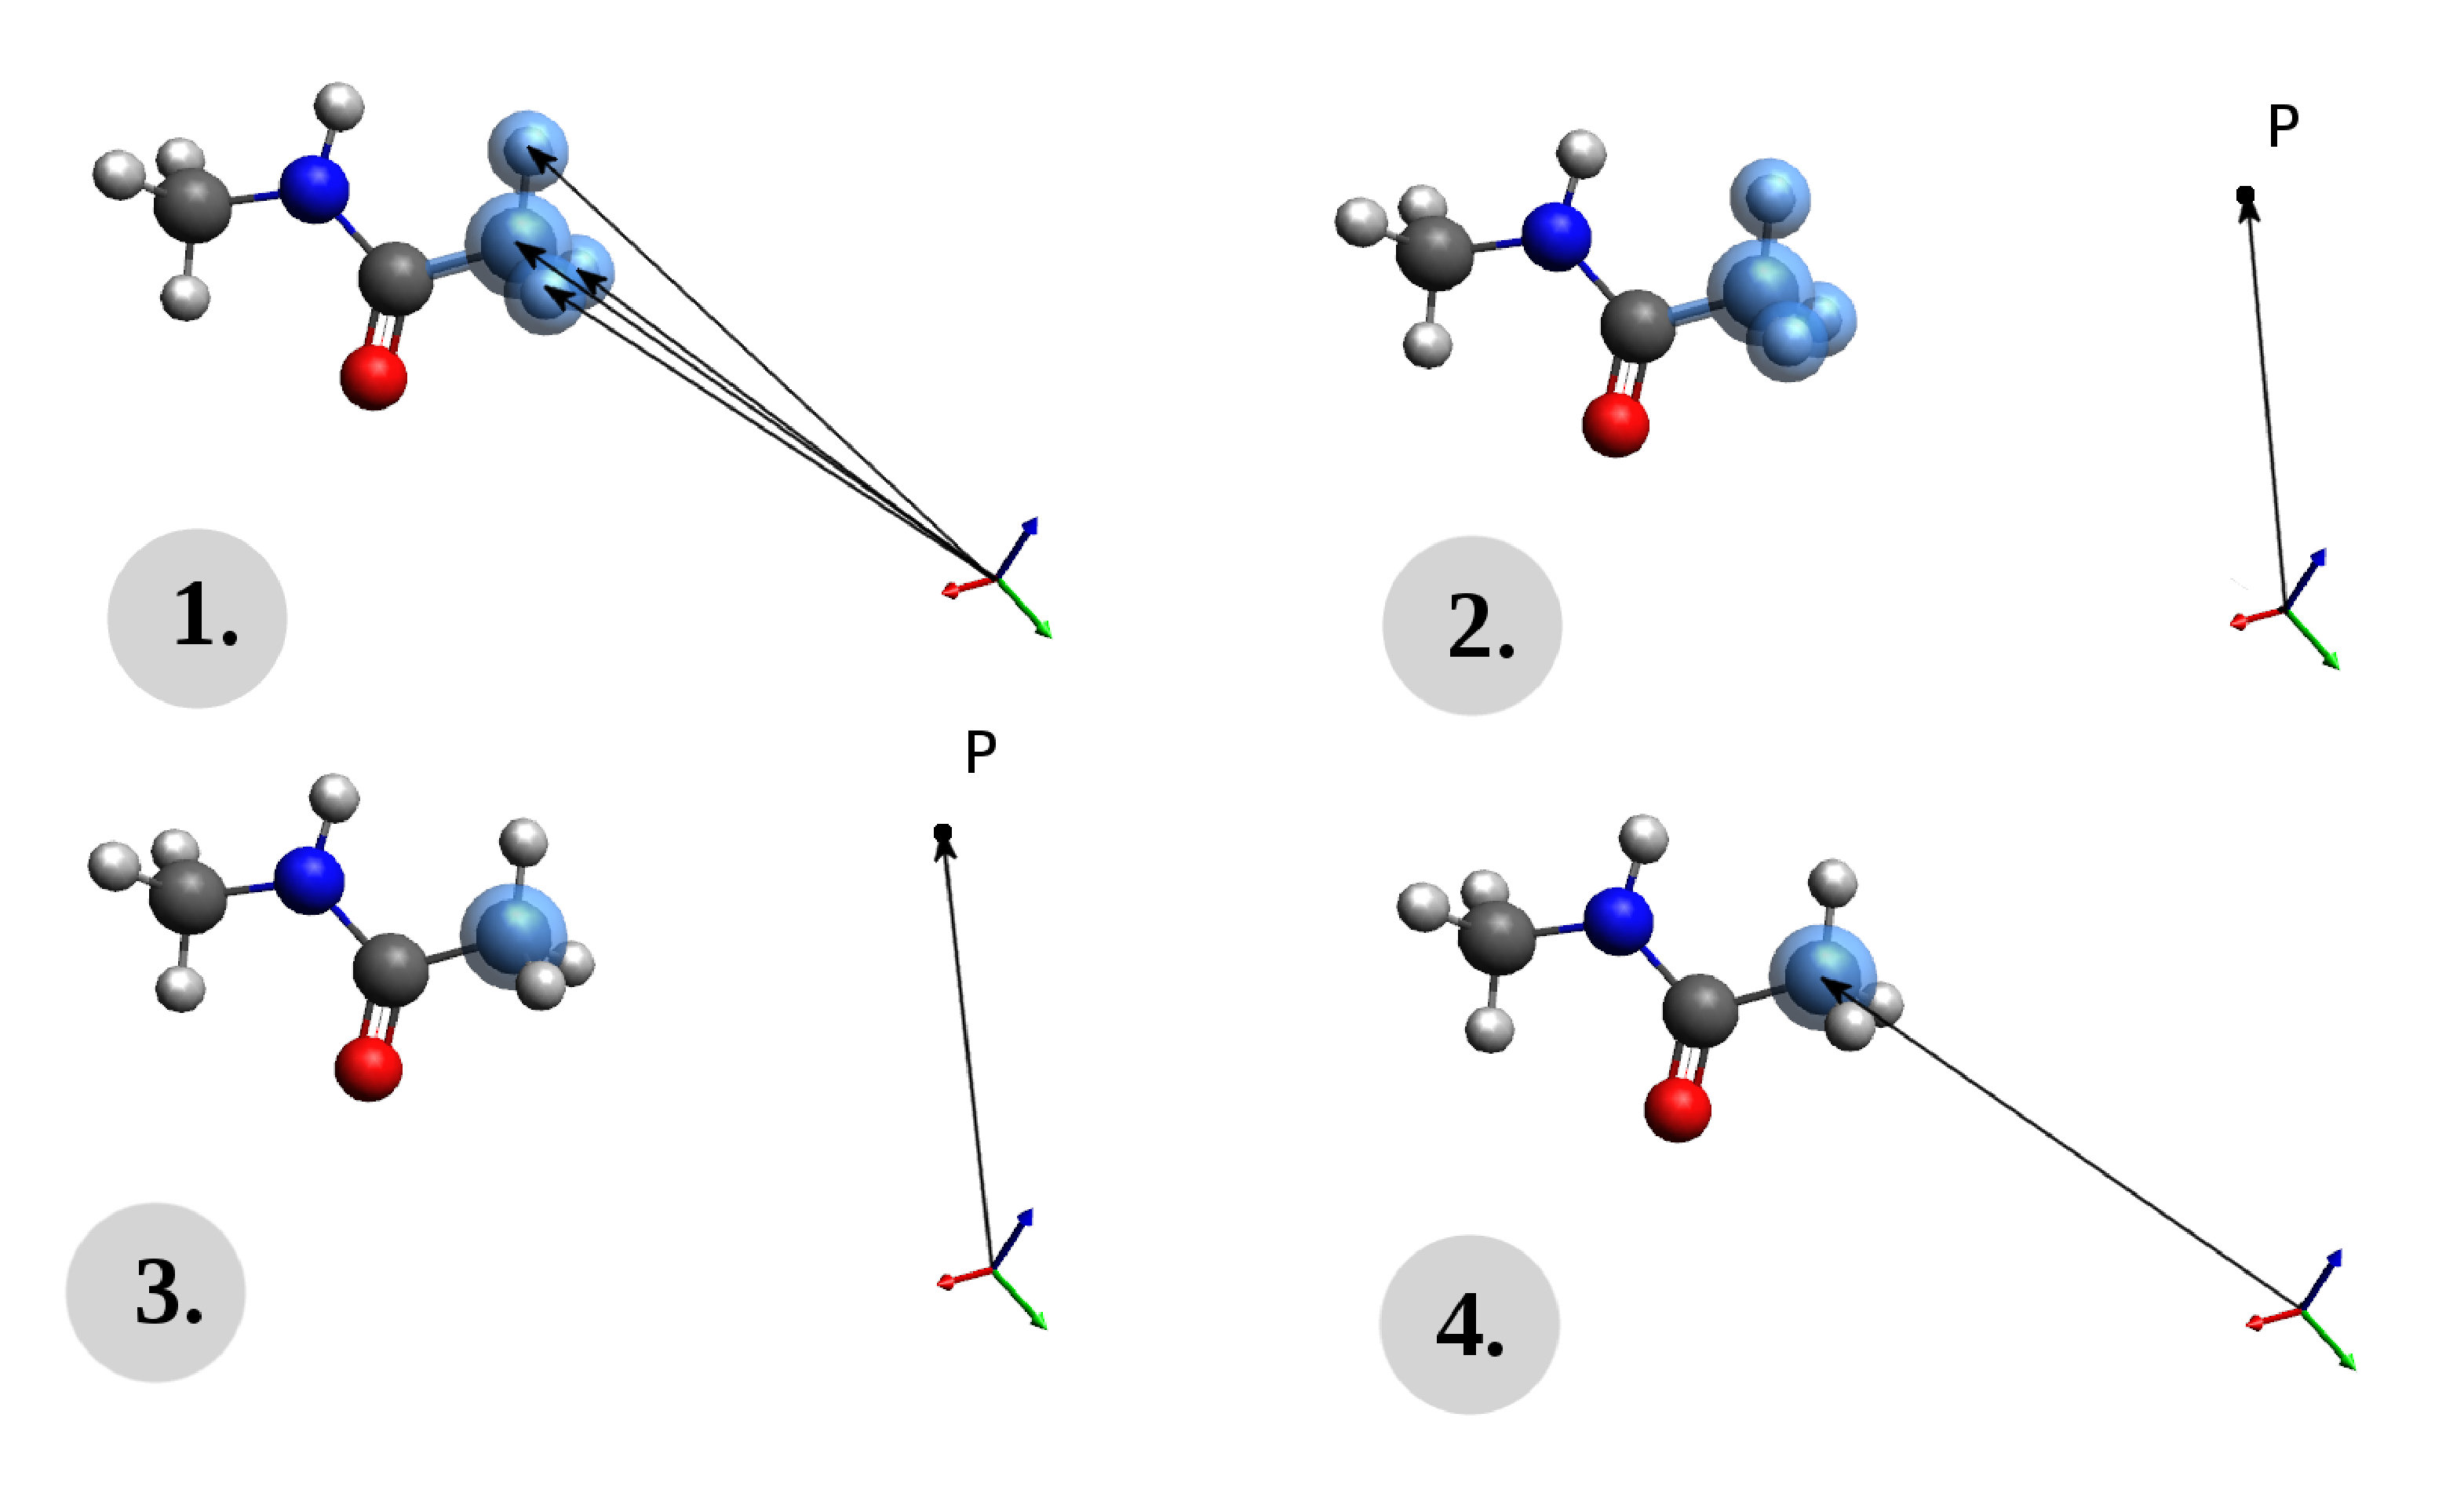
\includegraphics[width=0.9\linewidth]{contr.eps}
}
\caption{Construction of contracted SolCAMM-$n$ models. Here, as an example, we present
the construction of versions of SolCAMM-$12$ (or SolDMA-$12$) model for NMA. 
The example is shown for one of methyl groups which we approximate by a united atom 
placed on the corresponding carbon atom. The origins are depicted by arrows
whereas the multipole centers as blue spheres. 1) all the distributed multipoles 
are placed on each atom. Since they have different origins the cannot be summed up 
to obtain united atom. 2) Thus, it is necessary to shift their origins to one, 
arbitrary point P. From now on, all the multipoles have the same origin at P 
and they are additive. 3) All the multipoles for methyl group (four sets 
of multipoles for each atom) are summed over. The resulting united atom 
multipole moment has its origin at point P. 4) The center of these multipoles 
is moved to the carbon atom position.
\label{f:contr}}
\end{figure}
%

\begin{wrapfigure}{r}{0.30\textwidth}
\vspace{-30pt}
\begin{center}
    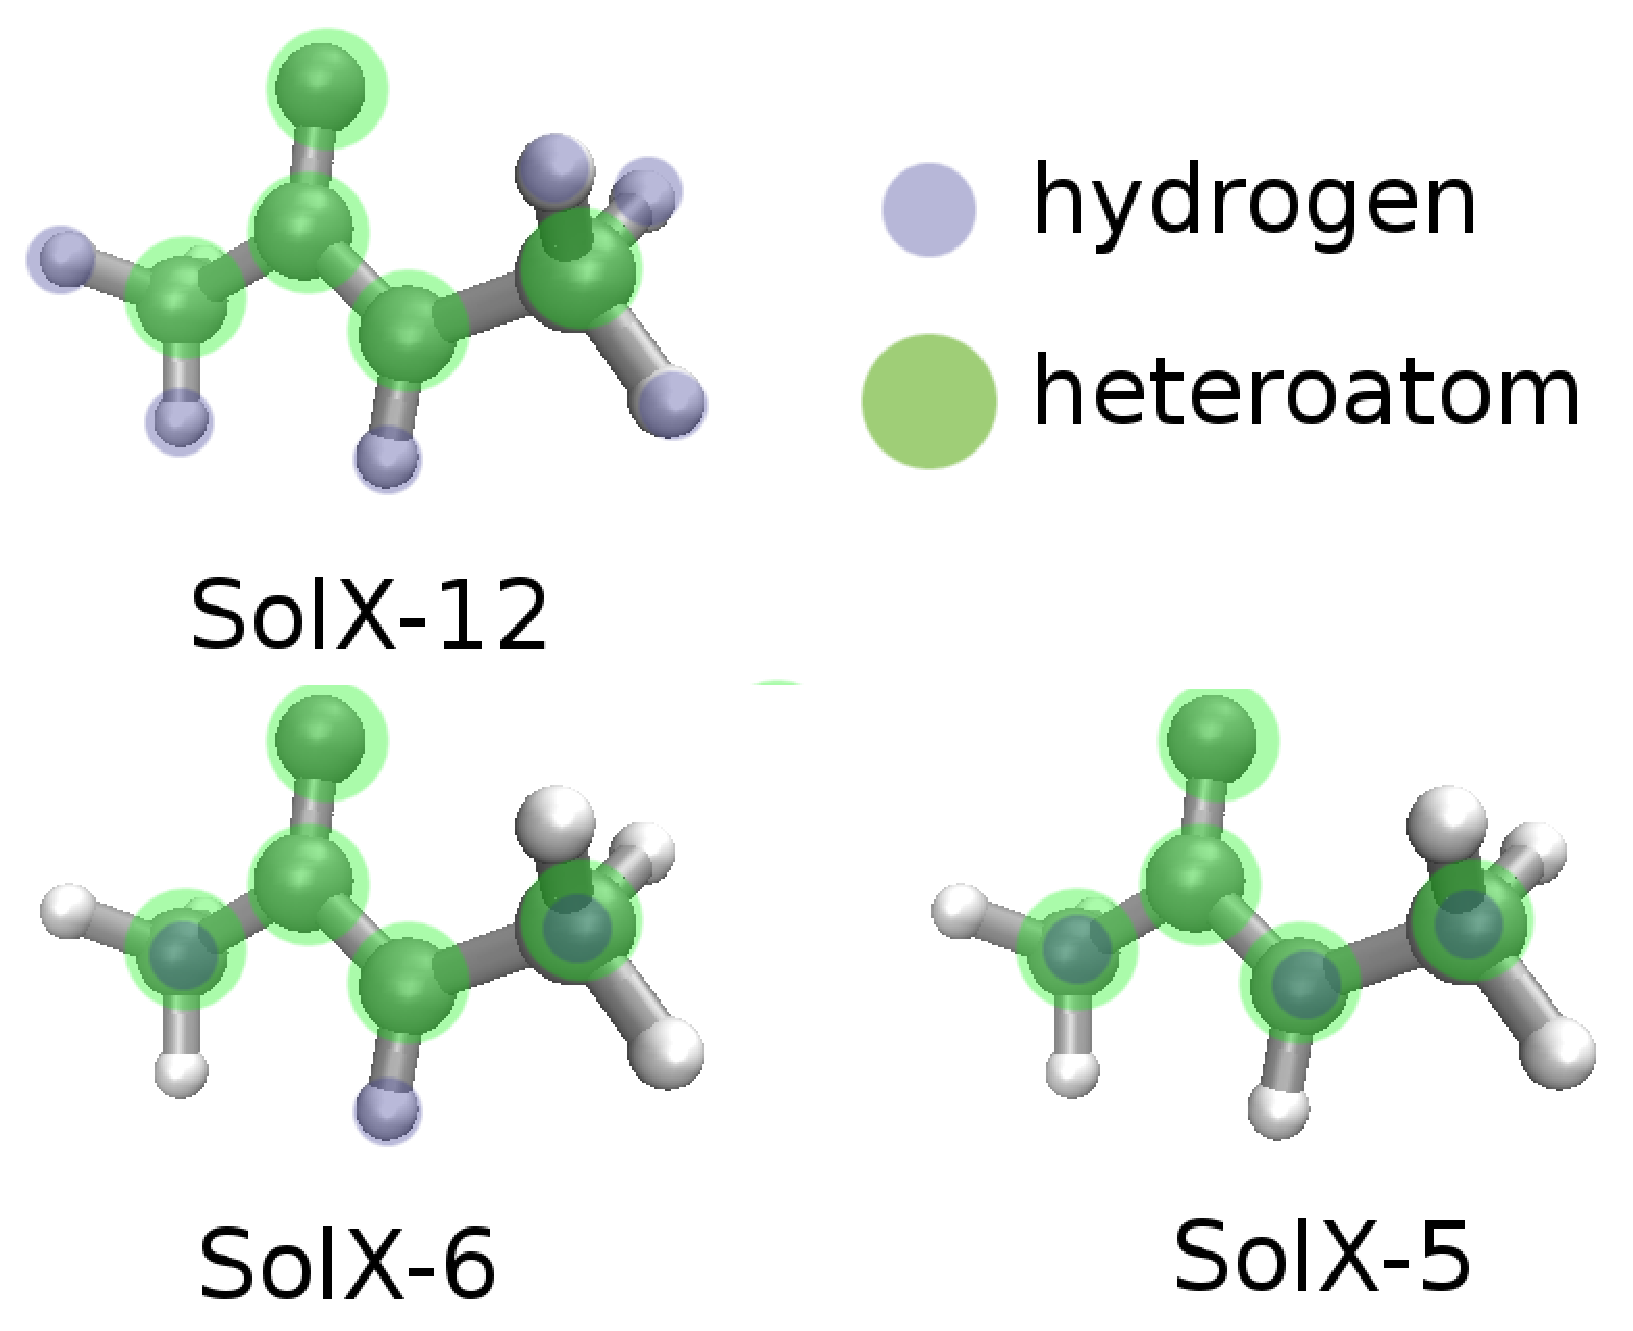
\includegraphics[width=0.28\textwidth]{SolXn.eps}
  \end{center}
  \vspace{-18pt}
  \caption{Variants of SolX models for $N$-methyl acetamide amide I mode.
X denotes distributed atomic multipoles in this case (e.g., DMA or CAMM).\label{f:solxn}}
\vspace{-20pt}
\end{wrapfigure}
%
\noindent This procedure can lead to the increase in the performance
of the method because the number of distributed centers
is decreased. If the contraction involves atoms that 
are not affected by the vibrational mode of interest (e.g. 
hydrogen atoms in the methyl group when one is interested
in amide I mode) the contracted models give basically 
the same results as uncontracted models (we 
will discuss it in the next Chapter). 

\subsection{SolEFP, SolEDS and SolSAPT models}

To include also non\hyp{}Coulombic effects to describe 
the intermolecular interaction potential one can use, for example,
the following methods:
%
\begin{enumerate}
  \item Effective Fragment 
Potentials\citep{Day.Jensen.Gordon.Webb.Stevens.Krauss.Garmer.Basch.Cohen.JCP.1996,
Flick.Kosenkov.Hohenstein.Sherrill.Slipchenko.JCTC.2012} (EFP)
  \item Variational\hyp{}perturbational Interaction Energy Decomposition
Scheme\citep{Sokalski.Roszak.Pecul.CPL.1988,
Chalasinski.Szczesniak.MolPhys.1988,Cybulski.Chalasinski.Moszynski.JCP.1990,
Gora.Bartkowiak.Roszak.Leszczynski.JCP.2004} (EDS)
  \item Symmetry Adapted Perturbation Theory\citep{Jeziorski.Moszynski.Szalewicz.ChemRev.1994} (SAPT)
\end{enumerate}
%
These will lead to the SolEFP, SolEDS and SolSAPT methods, accordingly. 
SolEFP method was already described in the previous sections
and the frequency shift is given as
%
\begin{equation} \label{e:dw-solefp}
\Delta\omega^{\rm SolEFP} = 
\Delta\omega^{\rm Coul} + \Delta\omega^{\rm Ex-Rep} + 
\Delta\omega^{\rm Ind} + \Delta\omega^{\rm Disp}_6 + \Delta\omega^{\rm CT}
\end{equation}
%
It is also strightforward to compute the 
solvation\hyp{}induced transition dipole change
with SolEFP vibrational forces according to the following prescription
%
\begin{equation} \label{e:dmu-solefp}
d = c!
\end{equation}
%

Due to its intrinsic fragmentation framework\citep{Gordon.Fedorov.Pruitt.Slipchenko.ChemRev.2012}, 
SolEFP is suitable for modeling very large systems
ranging from bulk solutions to highly heterogeneous
protein environments (see Chapter X). Note that in order
to compute the solvation\hyp{}induced frequency shift or the
transition dipole moment change, one needs the information
about the gas\hyp{}phase states of the molecules \emph{only}, 
because the effects of their interactions do not require 
any other specific solute\hyp{}solvent information.
On the other hand, according to 
previous sections, SolEFP espression in Eq.~\eqref{e:dw-solefp} 
is an approximation of the local mode approximation from
Eq.~\eqref{e:buckingham-2st-order-total-fund}. Let us 
explicitly list all the approximations here:
%
\begin{itemize}
 \item The charge\hyp{}penetration effects have been ignored, since they are likely to be weak. 
Nevertheless, since they were found to be of importance in describing Coulomb interaction energy 
(not frequency shift), such charge\hyp{}penetration effects need to be studied in the future.
 \item Due to the complexity of the SolEFP equations, we did not take into account the electric 
anharmonicity contributions, except for that associated with the Coulomb interaction\hyp{}induced 
frequency shift. When the exchange\hyp{}repulsion, induction, and dispersion terms in the frequency 
shift calculation are estimated, only the first derivatives of potential energy with respect 
to normal coordinates are considered. We already showed that this approximation is quite acceptable 
for describing the carbonyl and CN stretch modes.\citep{Blasiak.Cho.JCP.2014,Blasiak.Cho.JCP.2015,
Blasiak.Ritchie.Webb.Cho.XXX.2016}
However, for completeness it will be necessary to further test the validity of this approximation 
for other IR probes. In particular, we noticed that in the case of amide II mode
electronic anharmonicity of exchange\hyp{}repulsion contribution cannot be ignored.\citep{Blasiak.Cho.JCP.2015}
 \item The exchange\hyp{}repulsion interaction\hyp{}induced frequency shift was based on the approximation 
that only a single exchange of electron pair between solute and solvent is considered. 
In fact, it is believed here that this is an excellent approximation because the direct comparisons 
of the SolEFP results with completely \emph{ab initio}\footnote{SolEDS} calculation results indicate 
that the current SolEFP exchange\hyp{}repulsion frequency shifts are quite accurate.
 \item Induction and dispersion interaction\hyp{}induced frequency shifts 
were treated by taking into consideration only the dipole\hyp{}dipole interactions 
between LMO polarizable centers. Perhaps, the dispersion interaction\hyp{}induced 
contribution originating from distributed quadrupole\hyp{}dipole and quadrupole\hyp{}quadrupole 
interactions could be of importance as well.
 \item Since the SolEFP theory is to calculate all the vibrational solvatochromism parameters 
that can be obtained from \emph{ab initio} calculations of the solute molecule in the gas phase, 
the same structure should be used when the theory is applied to the solution systems 
with a solute molecule surrounded by solvent molecules. Therefore, there exists a certain 
ambiguity (difficulty) in perfectly superimposing it onto the solute molecule in solutions 
-- note that the detailed molecular structures (bond lengths, bond angles, and so on) 
of solute molecules in solutions are slightly different from that in the gas phase 
due to electronic structure change induced by solute\hyp{}solvent intermolecular interactions. 
Nevertheless, it should be emphasized that the present vibrational solvatochromism theory 
correctly includes the effects from solvation\hyp{}induced structural distortions 
since they are related to mechanical anharmonicity in the corresponding potential 
energy surface. Therefore, the above difficulty may not be the most crucial one, 
but still it needs to be investigated more in detail. We will refer to this issue as to
the \emph{superimposition problem}.
\end{itemize}
%
Thus, before SolEFP method is used, it has to be validated
first agaist some more accurate approach. 

%which is shown in Fig.~\ref{f:contr-uncontr-comparison}.
%%
%\begin{figure}[ht]
%\centering
%\setlength\fboxsep{0.4pt}
%\setlength\fboxrule{0.5pt}
%\fbox{
%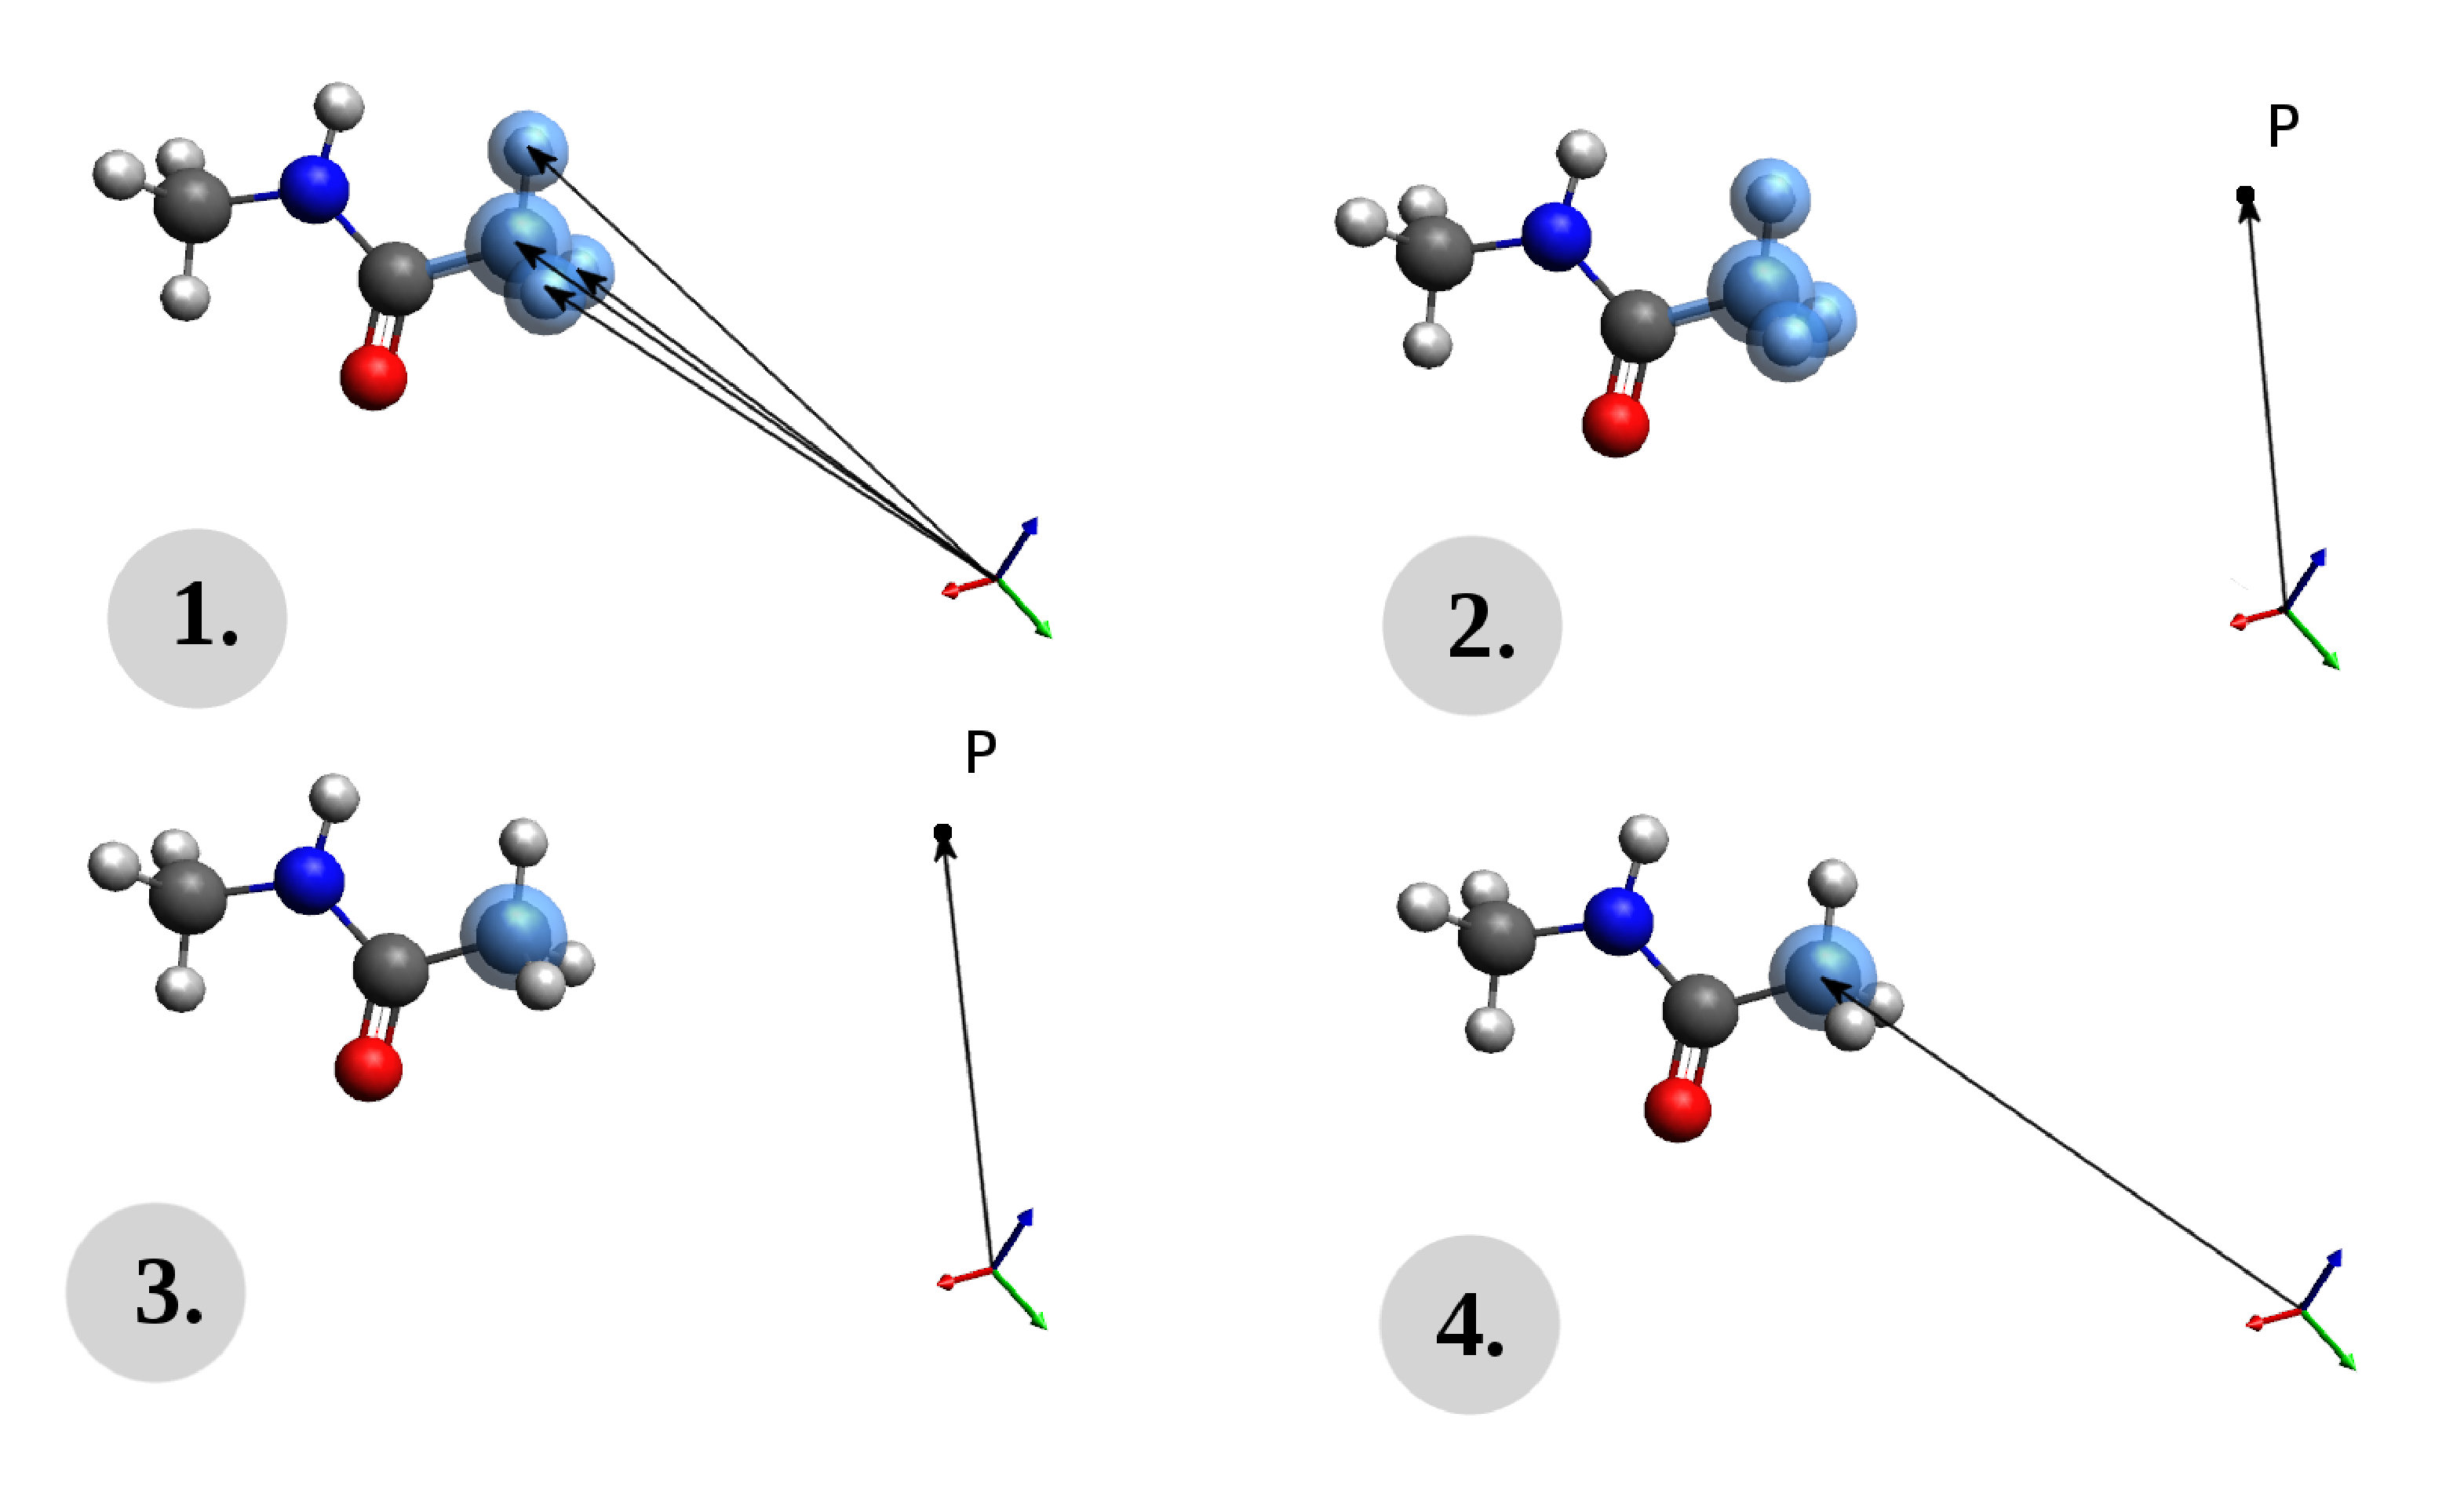
\includegraphics[width=0.1\linewidth]{contr.eps}
%}
%\caption{Performance of SolCAMM-12 (fully distributed) and SolCAMM-6 (two 
%united atoms) for the training set of NMA-H$_2$O$_n=1-30$ clusters.
%\label{f:contr-uncontr-comparison}}
%\end{figure}
%%
%


\printbibliography[heading=subbibintoc,title={References}]
\end{refsection}




\chapter{Future}

In this Thesis, we have focused primarily on changes of the vibrational
properties of solute molecules upon solvation. In this Chapter, 
we provide the scope of future perspectives of {\sc Solvshift}
as well as the underlying theory of electronic and magnetic solvatochromism.

\section{Electronic Solvatochromism}

Let us consider the change in the electronic energy levels
that occurs when solute molecule becomes solvated by $N$
solvent molecules. Let $\mathscr{H}_A$ denote the Hamiltonian
of isolated solute molecule with the associated 
eigenstates and eigenenergies according to the time\hyp{}independent
Schr{\:o}dinger equation:
%
\begin{subequations}
\begin{align}
\mathscr{H}_A \vert A_n \rangle &=  E^A_n \vert A_n \rangle \\
\mathscr{H}_B^{\zeta} \vert B_m^{\zeta} \rangle &=  E^{\zeta}_m \vert B_m \rangle
\end{align}
\end{subequations}
%
The interaction Hamiltonian reads
%
\begin{equation}
\mathscr{H}' = \sum_{\zeta} \mathscr{V}_{AB}^{\zeta} + \frac{1}{2} \sum_{\zeta\eta} \mathscr{V}_{BB}^{\zeta\eta}
\end{equation}
%
The change of the $n\leftarrow 0$ transition energy
due to solvation can be represented as
%
\begin{equation}
\Delta E^A_{n0}({\bf \overline{Q}}_A, U) = E^A_n({\bf \overline{Q}}_A, U) - E^A_0({\bf \overline{Q}}_A, U)
\end{equation}
%
where ${\bf \overline{Q}}_A$ denotes the solute's structure
in ground state normal mode representation and 
$U$ is the solute\hyp{}solvent interaction potential.
It is customary to relate the above energy change as a function of the 
gas\hyp{}phase molecular properties, rather than the properties 
in solution. Therefore, let us Taylor\hyp{}expand the energy change
around the solute's gas\hyp{}phase structure
%
\begin{multline}
\Delta E^A_{n0}({\bf \overline{Q}}_A, U) \cong \Delta E^A_{n0}({\bf Q}_A, U) + 
\sum_i  \fderiv{\Delta E^A_{n0}({\bf Q}_A, U)}{Q_i} 
\left( \overline{Q}_i - Q_i \right) 
\\
 \approx \Delta E^A_{n0}({\bf Q}_A, U) + 
\sum_i \frac{1}{M_i\omega_i^2} \fderiv{\Delta E^A_{n0}({\bf Q}_A, U)}{Q_i} \fderiv{U}{Q_i}
\end{multline}
%
where $M_i$ and $\omega_i$ denote the reduced mass and harmonic
frequency of solute in electronic ground state. Here we assume that
all the derivatives are evaluated at ${\bf {Q}}_A$ (gas\hyp{}phase).
Note that in the above expression we have not expanded with respect to
$U$ because the corresponding derivatives are very difficult to deal with.
To treat the effects of $U$ we shall use perturbation theory.

\subsection{Long-range approximation}

If the wavefunction overlap can be neglected, the electronic state
can be written as Hartree product of separate molecular eigenstates.

Before we consider the full many\hyp{}body ensemble, for the first approximation
let us consider the case when there is only
one solvent molecule, i.e., $\mathscr{H}'=\mathscr{V}_{AB}$.
From second\hyp{}order perturbation theory, the energy of $n$th electronic level
is given by
%
\begin{equation}
E_n = \langle A_nB_0 \vert \mathscr{H}' \vert A_nB_0 \rangle 
+ \sum_{k\ne n} \sum_{m\ne 0} \frac{
\lvert \langle A_nB_0 \vert \mathscr{H}' \vert A_kB_m \rangle  \rvert^2
}{E^A_{nk} + E^B_{0m}}
\end{equation}
%
It is straightforward to see that, in the first order, 
the energy change due to solvation when solute is in gas\hyp{}phase
structure is given by
%
\begin{multline}
\delta^{(1)} E^A_{n0}({\bf Q}_A, U) = \sum_{x} \Bigg\{ 
\left( q^A_{nn;x} - q^A_{00;x} \right) \phi({\bf r_x}) \\
+ \left( {\BM \mu}^A_{nn;x} - {\BM \mu}^A_{00;x} \right) \cdot \nabla \phi({\bf r_x})  
+ \frac{1}{3} \left( {\BM \Theta}^A_{nn;x} - {\BM \Theta}^A_{00;x} \right) \cdot \nabla \phi({\bf r_x}) 
+ \ldots
\Bigg\}
\end{multline}
%
where we multipole\hyp{}expanded the solute\hyp{}solvent interaction 
potential. For example, $q^A_{nn;x}$ denotes the monopole moment located at ${\bf r_x}$
that refers to the $n$th electronic state charge density distribution (nuclei + electrons).
Here, we assume first the vertical transition so that we can use the difference multipoles.
If the structure upon excitation changes, one can use different positions 
of distributed multipoles in both electronic states.
The total first\hyp{}order effect, including the structural distortion due to solute-solvent
interaction, can be expressed as
%
\begin{multline}
\delta^{(1)} E^A_{n0}({\bf \overline{Q}}_A, U) \cong \sum_{x} \Bigg\{ 
\left( q^A_{nn;x} - q^A_{00;x} \right) \phi({\bf r_x}) 
+ \left( {\BM \mu}^A_{nn;x} - {\BM \mu}^A_{00;x} \right) \cdot \nabla \phi({\bf r_x})  \\
+ \frac{1}{3} \left( {\BM \Theta}^A_{nn;x} - {\BM \Theta}^A_{00;x} \right) \cdot \nabla \phi({\bf r_x}) 
+ \ldots
\Bigg\} \\
%
+
%
\sum_{x} \sum_i \frac{1}{M_i\omega_i^2} \fderiv{U}{Q_i}
\Bigg\{ 
\fderiv{ q^A_{nn;x} }{Q_i} \phi({\bf r_x}) 
+ \fderiv{  {\BM \mu}^A_{nn;x}}{Q_i} \cdot \nabla \phi({\bf r_x})  
+ \frac{1}{3} \fderiv{ {\BM \Theta}^A_{nn;x} }{Q_i} \cdot \nabla \phi({\bf r_x}) 
+ \ldots
\Bigg\}
\end{multline}
%
in which we neglected the derivatives of electrostatic potential since they are 
a minor contribution.

Now, let us analyze the second order energy shift. This can also
be expanded as conventional interaction energy with making use
of static and dynamic imaginary frequency dependent polarizabilities.
However, such approach is not convenient because it is difficult
to compute the excited state polarizability by using distributed
site approach. Note that we aim in studying rather large molecules
for which single polarizable point is definitely not sufficient to
describe induction and dispersion effects.

Therefore, we try to use different approach and keep using the 
sum\hyp{}over\hyp{}states expression. Mainly,
%
\begin{equation}
\delta^{(2)} E^A_{n0}({\bf Q}_A, U) = 
\sum_{m\ne 0} 
\left[
\sum_{k\ne n}  \frac{ V_{n0,km}^2 }{E^A_{nk} + E^B_{0m}}
%
- \sum_{k\ne 0} \frac{
V_{n0,km}^2
}{E^A_{nk} + E^B_{0m}}
\right]
\end{equation}
%
where $V_{nk,0m}$ denotes the interaction between the 
solute's $k\leftarrow n$ transition density with
solvent's $m\leftarrow 0$ transition density. In principle,
such densities can be also multipole expanded (exchange effects should
be small compared to the electrostatic effects).
The price we have to pay is to deal with the sum that do not need to
converge fast. Here we hope that due to the increased number
of nodes of the excited state wave functions, the multipole
interactions will tend to cancel each other when raising the
quantum numbers in the summations. This is because
the integration is performed over the whole space, not
just over one molecule (like in the SOS evaluation of polarizability which
has significantly slow convergence).
If one could obtain a reasonable estimate of this second order 
effect by making use of transition multipoles (e.g. evaluated by TrCAMM) 
referring to the solute and solvent electronic
states, the model could be tested. One might also take into account
electronic states that has substantial oscillator strength. Note that
many electronic transitions have oscillator strengths that are
close to zero suggesting that
many terms in the above summations could be ignored.

The total second order energy shift is thus given by
%
\begin{multline}
\delta^{(2)} E^A_{n0}({\bf \overline{Q}}_A, U) \approx 
\sum_{m\ne 0} ^{m_{\rm Max}}
\left[
\sum_{k\ne n} ^{k_{\rm Max}} \frac{ V_{n0,km}^2 }{E^A_{nk} + E^B_{0m}}
%
- \sum_{k\ne 0} ^{k_{\rm Max}} \frac{
V_{n0,km}^2
}{E^A_{nk} + E^B_{0m}}
\right] \\
+
\sum_i \frac{1}{M_i\omega_i^2} \fderiv{U}{Q_i}
\sum_{m\ne 0} ^{m_{\rm Max}}
\Bigg\{
  2 \left[ 
\sum_{k\ne n} ^{k_{\rm Max}} \frac{ V_{n0,km} }{E^A_{nk} + E^B_{0m}} \fderiv{V_{n0,km} }{Q_i}
-
\sum_{k\ne 0} ^{k_{\rm Max}} \frac{ V_{n0,km} }{E^A_{nk} + E^B_{0m}} \fderiv{V_{n0,km} }{Q_i}
\right] \\
+
\left[
\sum_{k\ne n} ^{k_{\rm Max}} \ln (E^A_{nk} + E^B_{0m}) \fderiv{E^A_{nk}}{Q_i} V_{n0,km}^2
-
\sum_{k\ne 0} ^{k_{\rm Max}}  \ln (E^A_{nk} + E^B_{0m}) \fderiv{E^A_{nk}}{Q_i} V_{n0,km}^2
\right]
\Bigg\}
\end{multline}
%
Here, the structural distortion contribution
which is quite formidable, however, is straightforward. 
This contribution contains the energy and 
transition multipole (TrCAMM) first derivatives of the solute molecule with respect to
ground state vibrational coordinate. They can be evaluated
numerically without any problems. However, the tests need to be done in the future
to determine whether it is possible to choose ${m_{\rm Max}}$ and ${k_{\rm Max}}$
such that the sums are converged to a reasonable degree. 
If the fully electrostatic approximation is employed, 
the computation of first and second order energy shift 
is very fast and the time consumption can be considered as negligible.
Exchange\hyp{}repulsion, induction and dispersion effects
affect the energy shift through the vibrational forces
due to solvent and were already derived before
inthe SolEFP model of vibrational solvatochromism. 
Probably, those non\hyp{}Coulombic effects should be included
in the accurate energy shift calculation.



\subsection{Time-dependent response formalism}

Let us consider the dynamics of the electronic excitation 
by examining the time evolution of nuclear configuration and
electronic eigenstates (and spectrum of energies) when solvated molecule absorbs one photon
of electromagnetic energy. It is particularly important because
such phenomena can be studied by ultrafast time-resolved spectroscopy.
To be added later.

% ==================== APPENDICES ================================

\begin{appendices}
\addtocontents{toc}{\protect\setcounter{tocdepth}{0}}

\chapter{Molecular Vibrations\label{a:vibrational-analysis}}

To understand the theory of the vibrational solvatochromism 
discussed in detail in Section~\ref{s:theory}, it is customary
to be familiar with the theory behind the vibrational analysis
of a molecule build of $N$ atoms.

%\section{Matrix elements of $x^n$ operator in harmonic oscillator basis\label{a:matrix-elements}}
\section{The harmonic oscillator\label{a:harmonic-oscillator}}

\subsection{Some important matrix elements\label{a:matrix-elements}}

The following material is necessary for derivations of the Buckingham theory
of the vibrational frequency shifts that is presented in Sec.~\ref{s:buckingham-theory}. 

The matrix elements of the $x$ operator in the harmonic oscillator eigenstate basis set
can be found to be
%
\begin{equation}
\label{ea:mxn}
\langle n \vert \hat{x} \vert m \rangle = 
\sqrt{
\frac{\hbar}{2M\omega}
}
\left\{ 
   \sqrt{m+1} \delta_{n,m+1} + \sqrt{m} \delta_{n,m-1}
\right\}
\end{equation}
%
\noindent where $M$ is the reduced mass of the normal coordinate and $\omega$ is its 
angular frequency.

The evaluation of the matrix element of $\hat{x}^2=\hat{x}\hat{x}=\hat{x}\hat{1}\hat{x}$ 
operator is strightforward
by using the resolution of identity operator $\hat{1}$ and applying Eq.~\eqref{ea:mxn}
%
\begin{equation}
\langle n \vert \hat{x}^2 \vert m \rangle = 
\sum_{k=0}^{\infty} \langle n \vert \hat{x} \vert k \rangle \langle k \vert \hat{x} \vert m \rangle
\end{equation}
%
The final result is given by
%
\begin{multline}
\label{ea:mxxn}
\langle n \vert \hat{x}^2 \vert m \rangle = 
\frac{\hbar}{2M\omega}
\Big\{ 
   (2m+1) \delta_{n,m} + \sqrt{(m+1)(m+2)} \delta_{n,m+2} + \\
                         \sqrt{m(m-1)} \delta_{n,m-2}
\Big\}
\end{multline}
%
Following the same strategy one can easily find the expression for 
the matrix element of the $\hat{x}^3$ operator:
%
\begin{multline}
\label{ea:mxxxn}
\langle n \vert \hat{x}^3 \vert m \rangle = 
\left(
\frac{\hbar}{2M\omega}
\right)^{3/2}
\Big\{ 
   \sqrt{(m+1)(m+2)(m+3)} \delta_{n,m+3} + \\
   3(m+1)\sqrt{m+1} \delta_{n,m+1}
      +3m\sqrt{m}   \delta_{n,m-1} + \sqrt{m(m-1)(m-2)} \delta_{n,m-3}
\Big\}
\end{multline}
%
Note that diagonal matrix elements survive only for even operator $\hat{x}^2$
and vanish for all odd operators (it is true in generall for all $\hat{x}^n$
operators). Thus, when expansions up to the third order in $\hat{x}$ are 
used, the only surviving contribution is
%
\begin{equation}
\label{ea:mxm}
\langle n \vert \hat{x}^2 \vert n \rangle = 
\frac{\hbar}{2M\omega}(2n+1)
\end{equation}
%
and, of course, $\langle n \vert n \rangle=1$ term.

\section{Vibrational analysis of polyatomic molecule\label{asec:vibranal}}

The Hamiltonian of the vibrating molecule in equilibrium geometry under Born\hyp{}Oppenheimer approximation
can be expressed as follows:
\begin{equation}
\hat{H} = \sum_j \frac{1}{2\mu_j}\hat{{P}^2} + V({\bf Q})
\end{equation}
In the above equation, $V({\bf Q})$ denotes the vibrational potential energy function
expressed in normal coordinates, ${\bf Q}$. Under Harmonic approximation
\begin{equation}
V({\bf Q}) = \frac{1}{2} \sum_j \mu_j \omega_j^2 Q_j^2
\end{equation}
and the reduced mass $\mu_j$ corresponds to the $j$th normal coordinate $Q_j$ with
harmonic frequency $\omega_j$.

To find a set of coordinates $Q$ that are orthogonal to each other (i.e., describe the normal 
modes of the molecule) one needs to consider a quadratic potential energy function
\begin{equation}
V({\bf x}) = \frac{1}{2} \sum_i\sum_j \frac{\partial^2 E}{\partial x_i \partial x_j} x_i x_j
\end{equation}
and find such a silimarity transformation that
\begin{equation}\label{eq:pot_harm}
V({\bf Q}({\bf x})) = \frac{1}{2} \sum_j \mu_j \omega_j^2 Q_j^2({\bf x})
\end{equation}
or in matrix notation
\begin{equation}
V({\bf x}) = \frac{1}{2} {\bf x}^{\dagger} {\bf H}^{\rm Cart} {\bf x}  \quad \textrm{and   } V({\bf Q}({\bf x})) = \frac{1}{2} {\bf Q}^{\dagger} {\bf H}^{\rm Q} {\bf Q} 
\end{equation}
Obviously ${\bf H}^{\rm Q}$ is diagonal whereas ${\bf H}^{\rm Cart}$ is not. 

Let us assume that
\begin{equation}
{\bf Q} = {\bf L}^{\dagger} {\bf x}
\end{equation}
with ${\bf L}$ unitary.
Therefore it is clear that
\begin{equation}
V({\bf x}) = \frac{1}{2} {\bf x}^{\dagger} {\bf L} {\bf H}^{\rm Q} {\bf L}^{\dagger} {\bf x}
\end{equation}
or
\begin{equation}
{\bf H}^{\rm Q} = {\bf L}^{\dagger} {\bf H}^{\rm Cart} {\bf L}
\end{equation}
Therefore, diagonalizing ${\bf H}^{\rm Cart}$ one can find the orthogonal 
set ${\bf Q}$. We note that the dimensions of ${\bf x}$ and ${\bf Q}$ are the unit distances.

\section{Mass-weighted coordinates}

It is much better to express the normal coordinates in terms of the mass-weighted coordinates.
To see this, let us assume that we want to get the frequencies from Eq.\eqref{eq:pot_harm} by diagonalizing
the matrix ${\bf H}^{\rm Cart}$. Of course, we immediately obtain ${\bf L}$ and the force constants
in the normal modes expressed as cartesian displacements (${\bf Q}$). But note that these force constants 
contain \emph{unknown} reduced masses.
Therefore the determination of vibrational harmonic frequencies is not yet possible. 

However, one could 
associate the reduced mass with the definition of the normal coordinate.
Let us try with changing to the cartesian mass\hyp{}weighted coordinates defined by
\begin{equation}
\tilde{\bf x} = {\bf M}{\bf x} 
\end{equation}
with
\begin{equation}
M_{ij} = \delta_{ij} \sqrt{m_i}
\end{equation}
and rewrite the equations from Sec.\ref{asec:vibranal}.

By inserting ${\bf x}={\bf M}^{-1}\tilde{\bf x}$ we get
\begin{equation}
V(\tilde{\bf x}) = \frac{1}{2} \tilde{\bf x}^{\dagger} {\bf H}^{\rm MWC}  \tilde{\bf x}
\end{equation}
This corresponds to 
\begin{equation}
V(\tilde{\bf Q}) = \frac{1}{2} \tilde{\bf Q}^{\dagger} {\bf H}^{\rm MWC,Q}  \tilde{\bf Q}
\end{equation}
expressed in \emph{mass-weighted} normal coordinates defined by
\begin{equation}
\tilde{Q}_j = \sqrt{\mu_j} Q_j
\end{equation}
and with 
\begin{equation}
H_{ij}^{\rm MWC,Q} = \delta_{ij} \omega_j^2
\end{equation}
Therefore, diagonalizing mass-weighted Hessian in cartesian coordinates (${\bf H}^{\rm MWC}$)
we can easily obtain the frequencies since they are equal to $\omega_j=\sqrt{H_{jj}^{\rm MWC,Q}}$.
Because we also have
\begin{equation}
{\bf H}^{\rm MWC,Q} = \tilde{\bf L}^{\dagger} {\bf H}^{\rm MWC} \tilde{\bf L}
\end{equation}
we can immediately find that
\begin{equation}
\tilde{\bf x} = \tilde{\bf L} \tilde{\bf Q}
\end{equation}
or in cartesian not-weighted coordinates
\begin{equation}
{\bf x} = {\bf M}^{-1} \tilde{\bf L} \tilde{\bf Q} = {\bf l} \tilde{\bf Q}
\end{equation}
where we introduced the matrix ${\bf l}={\bf M}^{-1} \tilde{\bf L}$.

%--------------------------------------------------------------------------------------------------
\chapter{Correction terms for the evaluation of $\Delta \omega^{\rm Coul}$\label{a:fk-terms}}

Here we list the explicit formulae for the evaluation of the first and second derivatives
of the solute\hyp{}solvent interaction potential that emerge due to the electrostatic potential
variation along the solute's normal coordinate. Subsequenty, the series 
convergence properties are tested for model NMA-H$_2$O dimers. 
Refer to Eq.~\eqref{e:dw-solefp-coul-correction}
for the context.

\section{Asymptotic analysis of the correction terms}

After inserting the series expansions from Eq.~\eqref{e:potential-gradients} 
and Eq.~\eqref{e:interaction-tensors} into Eqs.~\eqref{e:f-terms} and \eqref{e:k-terms}
one can easily see that each term containing interaction tensors of various ranks
will have different asymptotic behaviours which can be put in 
the following rule:
%
\begin{quote}
The term containing interaction tensor of rank $n$ 
has $r^{-(n+1)}$ asymptotic dependence.
\end{quote}
%
Following this rule,
it is easy to see that considering the dependence up to $r^{-4}$ among the new terms
there are two $r^{-2}$ terms, five $r^{-3}$ terms and eight
$r^{-4}$ terms, so fifteen terms in total. Comparing with 
solvatochromic multipole terms when one has two $r^{-1}$,
four $r^{-2}$, six $r^{-3}$ and eight $r^{-4}$ terms (20 in total)
the amount of the new terms is quite big though there are no $r^{-1}$ 
terms present. In Table~\ref{t:cterms} all the terms for $n=2,3,4$
are listed.

\begin{table}[ht]
%\resizebox{1.4\textwidth}{!}{\begin{minipage}{\textwidth}
\caption{List of the additional terms originating from the
electrostatic interaction that were not included in $\Delta\omega^{\rm SolDMA}$.
Here, the subscripts or superscripts $x$ and $y$ refer to the distributed multipole
sites of the solute and solvent molecules, respectively. To simplify notation,
we used the definitions: $G^{(i)}_{xy} \equiv {\bf L}_x^{(i)} \cdot {\bf r}_{xy}$,
$G_{x;xy} \equiv {\BM \mu}_x \cdot {\bf L}_x^{(i)}$, $G_{y;xy} \equiv {\BM \mu}_y \cdot {\bf L}_x^{(i)}$
and $G_{x;xy}' \equiv \fderiv{{\BM \mu}_x}{Q_i} \cdot {\bf L}_x^{(i)}$.
It is assumed that the derivatives are computed at the solute's gas-phase geometry.
\label{t:cterms}}
%\begin{footnotesize}
\begin{tabular*}{1.0\textwidth}{@{\extracolsep{\fill} } l ll ll}
\hline\hline
$r^{-n}$        && $U_i^{(x,y)}$   && $U_{jj}^{(x,y)}$ \\%[10ex] 
\hline
$r^{-2}$        && $-q_xq_y r_{xy}^{-3} G^{(i)}_{xy}$  
                && $-2\fderiv{q_x}{Q_i}q_y r_{xy}^{-3} G^{(i)}_{xy}$ \\
\hline
\multirow{3}{*}{$r^{-3}$}  && $-3G^{(i)}_{xy} r_{xy}^{-5} \left( q_x {\BM \mu}_y  -q_y {\BM \mu}_x \right) \cdot {\bf r}_{xy}$  
                           && $-6G^{(i)}_{xy} r_{xy}^{-5} \left( \fderiv{q_x}{Q_i} {\BM \mu}_y  -q_y \fderiv{{\BM \mu}_x}{Q_i} \right) \cdot {\bf r}_{xy}$ \\
                           && $r_{xy}^{-3} \left( q_x {\BM \mu}_y  -q_y {\BM \mu}_x \right) \cdot {\bf L}_x^{(i)}$ 
                           && $2r_{xy}^{-3} \left( \fderiv{q_x}{Q_i} {\BM \mu}_y  
                                                -q_y \fderiv{{\BM \mu}_x}{Q_i} \right) \cdot {\bf L}_x^{(i)}$ \\
                           && 
                           && $q_xq_y\left( 3\left(G^{(i)}_{xy}\right)^2 r_{xy}^{-2} - 
                                  \left| {\bf L}_x^{(i)} \right|^2\right)r_{xy}^{-3}$\\
\hline
\multirow{8}{*}{$r^{-4}$}  && $2r_{xy}^{-5} \left( q_x{\BM \Theta}_y + q_y{\BM \Theta}_x \right) : {\bf L}_x^{(i)} \otimes {\bf r}_{xy}$  
                           && $4r_{xy}^{-5} \left( \fderiv{q_x}{Q_i}{\BM \Theta}_y 
                              + q_y\fderiv{{\BM \Theta}_x}{Q_i} \right) : {\bf L}_x^{(i)} \otimes {\bf r}_{xy}$ \\
                           && $-5G^{(i)}_{xy} r_{xy}^{-7} \left( q_x{\BM \Theta}_y 
                              + q_y{\BM \Theta}_x \right) : {\bf r}_{xy} \otimes {\bf r}_{xy}$ 
                           && $-10G^{(i)}_{xy} r_{xy}^{-7} \left( \fderiv{q_x}{Q_i}{\BM \Theta}_y 
                              + q_y\fderiv{{\BM \Theta}_x}{Q_i} \right) : {\bf r}_{xy} \otimes {\bf r}_{xy}$\\
                           && $-3\left(G^{(i)}_{xy} {\BM \mu}_x \cdot {\BM \mu}_y
                              + G_{y;xy} {\BM \mu}_x \cdot {\bf r}_{xy}
                                     \right)r_{xy}^{-5}$ 
                           && $-6\left(G^{(i)}_{xy} \fderiv{{\BM \mu}_x}{Q_i} \cdot {\BM \mu}_y
                              + G_{y;xy} \fderiv{{\BM \mu}_x}{Q_i} \cdot {\bf r}_{xy}
                                     \right)r_{xy}^{-5}$ \\
                           && $-3 G_{x;xy} r_{xy}^{-5} {\BM \mu}_y \cdot {\bf r}_{xy}$
                           && $-6 G_{x;xy}'r_{xy}^{-5} {\BM \mu}_y \cdot {\bf r}_{xy}$ \\
                           && $15G^{(i)}_{xy} r_{xy}^{-7} {\BM \mu}_x \otimes {\BM \mu}_y : {\bf r}_{xy}^2 $ 
                           && $30G^{(i)}_{xy} r_{xy}^{-7} \fderiv{{\BM \mu}_x}{Q_i} \otimes {\BM \mu}_y : {\bf r}_{xy}^2 $\\
                           && 
                           && $15r_{xy}^{-7} \left(G^{(i)}_{xy}\right)^2 \left( q_x{\BM \mu}_y 
                              - q_y{\BM \mu}_x \right) \cdot {\bf r}_{xy} $ \\
                           &&  
                           && $-3q_x r_{xy}^{-5} \left( 2G^{(i)}_{xy} {\bf L}_x^{(i)} 
                              + \left(G^{(i)}_{xy}\right)^2 \right) \cdot {\BM \mu}_y $ \\
                           &&  
                           && $+3q_y r_{xy}^{-5} \left( 2G^{(i)}_{xy} {\bf L}_x^{(i)} 
                              + \left(G^{(i)}_{xy}\right)^2 \right) \cdot {\BM \mu}_x $ \\
\hline\hline
\end{tabular*}
%\end{footnotesize}
%\end{minipage} }
\end{table}


\section{Analysis of the convergence properties of Eq.~\eqref{e:dw-solefp-coul-correction}\label{a:convergence-of-the-correction-terms}}

We have analyzed the various contributions to $\Delta\omega^{\rm Coul}(\partial\phi)$
for the three model systems A, B and C depicted in Fig.XXX. It is found 
(Table~\ref{t:ctest}) that
it is safe to truncate the series espansion on $r^{-2}$ terms. The other higher order terms,
especially in the case of the electronic anharmonicity contribution 
(associated with $U_{jj}$), can cause unreasonably
large frequency shifts. 
We compare the approximate evaluation with SolEDS calculations as a benchmark frequency shifts.

\begin{table}[ht]
\caption{Convergence of the electrostatic correction terms to SolCAMM
method that were estimated for three model NMA-H$_2$O dimers
shown in Figure XXX. In this Table, 'MEA' and 'EA' denote the mechanical and electric
anharmonicity contributions, respectively, whereas 'Total' is their sum.
Cumulative atomic multipole moments (CAMM) were evaluated 
at all atoms of NMA with subsecuent contraction of CH$_3$ groups 
to get SolCAMM-6 model.
Calculations were performed at HF/6-311++G(d,p) level.
All values are given in cm$^{-1}$.
\label{t:ctest}}
\begin{tabular*}{1.0\textwidth}{@{\extracolsep{\fill} } l ll ll}
\hline\hline
\multicolumn{5}{c}{Amide I mode} \\
\hline
System               & Method    & MEA           & EA         & Total        \\
\hline
\multirow{5}{*}{A}   & SolCAMM   & -39.4 (+6.2)  & 5.3 (+0.9) & -34.1 (+7.1) \\
        & Corr$^{\rm r2}$        & -47.4 (-1.8)  & 4.9 (+0.5) & -42.5 (-1,3) \\
        & Corr$^{\rm r2+r3}$     & -53.2 (-7.6)  & 7.7 (+3.3) & -45.5 (-4.3) \\
        & Corr$^{\rm r2+r3+r4}$  & -55.3 (-9.7)  & 8.8 (+4.4) & -46.5 (-5.3) \\
                     & SolEDS    & -45.6         & 4.4        & -41.2        \\
\hline
\multirow{5}{*}{B}   & SolCAMM   & -15.2 (+1.7)  & 3.8 (+2.2) & -11.4 (+3.9) \\
        & Corr$^{\rm r2}$        & -17.7 (-0.8)  & 4.3 (+2.7) & -13.4 (+1.9) \\
        & Corr$^{\rm r2+r3}$     & -21.1 (-4.2)  & 4.0 (+2.4) & -17.1 (-1.8) \\
        & Corr$^{\rm r2+r3+r4}$  & -21.2 (-4.3)  & 3.7 (+2.1) & -17.5 (-2.2) \\
                     & SolEDS    & -16.9         & 1.6        & -15.3        \\
\hline
\multirow{5}{*}{C}   & SolCAMM   & -35.4 (+6.6)  & 8.9 (+3.3) & -26.5 (+9.9) \\
        & Corr$^{\rm r2}$        & -40.7 (+1.3)  & 8.8 (+3.2) & -31.9 (+4.5) \\
        & Corr$^{\rm r2+r3}$     & -41.6 (+0.4)  &11.9 (+6.3) & -29.7 (+6.7) \\
        & Corr$^{\rm r2+r3+r4}$  & -42.6 (-0.6)  &15.0 (+9.4) & -27.6 (+8.8) \\
                     & SolEDS    & -42.0         & 5.6        & -36.4        \\
\hline\hline
\multicolumn{5}{c}{Amide II mode} \\
\hline
System               & Method    & MEA           & EA         & Total        \\
\hline
\multirow{5}{*}{A}   & SolCAMM   & 14.0 (+2.9)   & -6.3 (-3.2)& 7.7 (-0.3)   \\
        & Corr$^{\rm r2}$        & 14.3 (+3.2)   & -6.4 (-3.3)& 7.9 (-0.1)   \\
        & Corr$^{\rm r2+r3}$     & 14.0 (+2.9)   & -7.2 (-4.3)& 6.8 (-1.2)   \\
        & Corr$^{\rm r2+r3+r4}$  & 15.0 (+3.9)   & -8.2 (-5.1)& 6.8 (-1.2)   \\
                     & SolEDS    & 11.1          & -3.1       & 8.0          \\
\hline
\multirow{5}{*}{B}   & SolCAMM   & 10.6 (-1.1)   & 13.2 (+8.4)& 23.8 (+7.3)  \\
        & Corr$^{\rm r2}$        & 13.4 (+1.7)   & 13.2 (+8.4)& 26.6 (+10.1) \\
        & Corr$^{\rm r2+r3}$     & 19.1 (+7.4)   & 22.0 (+17.2)&41.1 (+24.6) \\
        & Corr$^{\rm r2+r3+r4}$  & 21.6 (+9.9)   & 42.1 (+37.3)&63.7 (+47.2) \\
                     & SolEDS    & 11.7          & 4.8        & 16.5         \\
\hline
\multirow{5}{*}{C}   & SolCAMM   & 12.8 (+1.2)   & -4.9 (-2.9)& 7.9 (-1.7)   \\
        & Corr$^{\rm r2}$        & 14.4 (+2.8)   & -4.9 (-2.9)& 9.5 (-0.1)   \\
        & Corr$^{\rm r2+r3}$     & 14.6 (+3.0)   & -5.4 (-3.4)&11.0 (+1.4)   \\
        & Corr$^{\rm r2+r3+r4}$  & 14.7 (+3.1)   & -5.6 (-3.6)& 9.1 (-0.5)   \\
                     & SolEDS    & 11.6          & -2.0       & 9.6          \\
\hline\hline
\end{tabular*}
\end{table}
%--------------------------------------------------------------------------------------------------

\begin{refsection}
\chapter{Distributed multipole analysis\label{c:dma}}

In this Thesis we make use of distributed multipole 
moments determined by using various methods in order to obtain
the appropriate vibrational solvatochromic midels. In this Chapter,
we describe the mathematical formulation and characteristics of various methods
in more detail.
Under the distributed multipole approximation, the Coulombic
interaction energy can be expressed as a following series\citep{Stone.TheTheoryOfIntermolecularForces.1996}
%
\begin{equation}
 U^{\rm Coul} = \sum_{x\in A}\sum_{y\in B} \cong T^{xy}q^{(x)}q^{(y)} + 
\sum_\alpha T^{xy}_\alpha \left( q^{(x)} \mu^{(y)}_\alpha - \mu^{(x)}_\alpha q^{(y)}\right)
 - \sum_{\alpha\beta} T^{xy}_{\alpha\beta} \mu^{(x)}_\alpha \mu^{(y)}_\beta + \ldots
\end{equation}
%
where $x$ and $y$ denote the distributed sites on the solute and solvent
molecules, respectively. There exists a number of ways of obtaining
the distributed multipoles. 

\section{DMA method}

In the distributed multipole analysis 
(DMA) of Stone\citep{Stone.JCTC.2005}, the particular multipoles
are computed by integrating the matrix elements of multipole
operators over localized amount of volume enclosing the distributed
site of interest. These multipoles are characterized by good convergence
properties of the resulting interaction energies. 
However, differentiation of DMA with respect to nuclear coordinate
is difficult to implement (the integration domains need to be the same
during numerical computation of the derivatives). 

\section{CAMM method}

More convenient in use in the vibrational solvatochromic calculations
is the cumulative atomic multipole
moments method (CAMM) developed by Sokalski and Poirier.\citep{Sokalski.Poirier.CPL.1983}
The multipoles are the generalization of the Mulliken atomic charges
and they are given by exact relations:
%
\begin{equation}
\begin{aligned}
q_x              &=-\sum_{r\in x} \sum_s  P_{rs} \langle r \rvert s \rangle \\
\bm{\upmu}_x     &= \sum_{r\in x} \sum_s  P_{rs} 
\left[
        \langle r \rvert s \rangle {\bf R}_x - \langle r \lvert {\bf r} \rvert s \rangle
\right]   \\
\bm{\Theta}_{x}  &= \sum_{r\in x} \sum_s P_{rs}
\left[
   - {\bf R}_x \otimes {\bf R}_x \langle r \rvert s \rangle +
    {\bf R}_x \otimes  \langle r \lvert {\bf r} \rvert s \rangle + 
                       \langle r \lvert {\bf r} \rvert s \rangle \otimes {\bf R}_x -
    \langle r \lvert {\bf r} \otimes {\bf r} \rvert s \rangle
\right]   \\
%\begin{gathered}
\bm{\Omega}_{x}  &=
\sum_{r\in x} \sum_s P_{rs}
\Big[
          {\bf R}_x \otimes {\bf R}_x \otimes {\bf R}_x \langle r \rvert s \rangle -
          {\bf R}_x \otimes {\bf R}_x \otimes \langle r \lvert {\bf r} \rvert s \rangle -
          {\bf R}_x \otimes \langle r \lvert {\bf r} \rvert s \rangle \otimes {\bf R}_x \\ \nonumber
 &\quad- \langle r \lvert {\bf r} \rvert s \rangle \otimes {\bf R}_x \otimes {\bf R}_x +
          {\bf R}_x \otimes \langle r \lvert {\bf r} \otimes {\bf r} \rvert s \rangle +
          \langle r \lvert {\bf r} \otimes {\bf R}_x \otimes {\bf r} \rvert s \rangle +
          \langle r \lvert {\bf r} \otimes {\bf r} \rvert s \rangle \otimes {\bf R}_x \\ \nonumber
 &\quad- \langle r \lvert {\bf r} \otimes {\bf r} \otimes {\bf r} \rvert s \rangle
\Big] 
%\end{gathered}
\end{aligned}
\end{equation}
%
where $r$ and $s$ denote the basis functions, $P_{rs}$ is the
one\hyp{}particle density matrix element and $x$ is the atomic centre.
All the one\hyp{}electron multipole integrals 
$\langle r \lvert f({\bf r},{\bf R}_x)\rvert s \rangle$ 
can be easily 
evaluated by a computer program using the above analytical formulae.
Therefore, there is no technical problem related to the differentiation of CAMM
with respect to the nuclear coordinate.\footnote{One needs to pay attention
upon keeping the origins of multipoles fixed during the numerical differentiation;
see the discussion on that aspect in Sec.XXX} However, the convergence of CAMM
is somewhat worse than that of DMA since the integration of matrix elements 
is performed over the whole space. This means that the electronic density
is divided evenly over all atomic orbitals, even those which are located far
from the distribution center. Nevertheless, CAMM still provides reasonable 
estimates of $U^{\rm Coul}$ and we shall use them throughout this Thesis.

\section{LMTP method}

Instead of using atoms as expansion centers, one can use also localized molecular orbitals
for that purpose. This is the localized orbital multipole (LMTP) expansion 
proposed by Etchebest \emph{et al}.\citep{Etchebest.Lavery.Pullman.TheorChimActa.1982}
The aim is to decompose molecular multipole moments into additive
distributed moments which are centered not only at atomic sites
(and even at mid\hyp{}bond distances) but also at lone\hyp{}pairs 
and extended $\pi$\hyp{}orbitals in a way similar to the Mulliken\hyp{}based
partitioning scheme.

The momecular primitive and origin\hyp{}dependent multipole moment $\bf M$
is given as:
%
\begin{equation}\label{M}
{\bf M} = \sum_A Z_A{\bf R}_A + \tbraket{\Psi}{\mathscr{M}^{(r)}}{\Psi}
\end{equation}
%
where $\mathscr{M}^{(r)}$ is $r$-th rank multipole moment operator
%
\begin{equation}\label{Mop}
\mathscr{M}^{(r)} = -\sum_i^N \underbrace{{\bf r}_i \otimes \cdots \otimes {\bf r}_i }_{r \; {\rm times}} = \sum_i^N \hat{m}^{(r)}(N)
\end{equation}
%
The summations extend over all $A$ atoms and all electrons $i$ in the system
and $\otimes$ is tensor outer product operator.
Using Slater\hyp{}Condon rule for matrix elements of one\hyp{}electron operator
between ground state bra and ket Slater determinants we obtain
%
\begin{equation}\label{MSC}
{\bf M} = \sum_A Z_A{\bf R}_A - \sum_i^N \tbraket{\chi_i}{\hat{m}^{(r)}(1)}{\chi_i}
\end{equation}
%
and $\ket{\chi_i}$ are occupied molecular spin\hyp{}orbitals.
Now let us define a simple decomposition of electronic part of $\bf M$, i.e. ${\bf M}_e$:
%
\begin{equation}\label{MSCp}
{\bf M}_e = \sum_G {\bf M}_{e,G} =  -\sum_G\sum_{i \in G} \tbraket{\chi_i}{\hat{m}^{(r)}(1)}{\chi_i}
\end{equation}
%
Now, if we want to start from canonical orbitals $\ket{\chi_i}_C$ and use atomic basis functions to create also
non\hyp{}atomic and non\hyp{}mid\hyp{}bond distributed moments one should rather use in Equation \eqref{MSCp} localized
molecular spin\hyp{}orbitals, $\ket{\chi_i}_L$:
%
\begin{equation}\label{a}
\ket{\chi_i}_L = \sum_j U_{ji} \ket{\chi_i}_C
\end{equation}
%
where $\bf U$ is unitary rotation matrix in space of canonical MOs which localizes them. Assuming we know
$U_{ji}$ elements and using LCAO expansion of canonical MO one immediately finds that
%
\begin{equation}\label{b}
{\bf M}_{e,G} = -\sum_{i \in G} \sum_{jm} \sum_{kl} U^*_{ji} U_{mi} C^*_{jl} C_{mk} \tbraket{l}{\hat{m}^{(r)}(1)}{k}
\end{equation}
%
Here, $C_{ij}$ are canonical expansion coefficients of MO in AO basis.

When we evaluate all the moments for each LMO group $G$ we can accumulate them in each $G$-th center
changing the origins. There are always MOs which are centered mainly on atoms (atomic contributions
mostly from core AOs) but there will be many nonatomic centers wich will contribute to bond, lone pair
as well as $\pi$\hyp{}orbital distributed moments, respectively. The centers can be grouped to reduce the number
of expansion centers. The part of $\bf M$ which comes from atomic
nuclei can be just added to electronic atomic moments.

\printbibliography[heading=subbibintoc,title={References}]
\end{refsection}

\chapter{Experiments\label{a:exp-ftir}}

Absorption frequencies of CN stretch modes in MeCN and MeSCN dissolved in various
solvents (Fig.~\ref{f.MeCN.MeSCN.vs.solvents}) were measured by using FTIR (Bruker VERTEX 70) 
spectrometer at 22{\degree}C with 1 cm$^{-1}$ 
resolution. In the cases of very weak solubility, the saturated solutions of Me(S)CN were 
prepared by ultrasonification (JEOITECH UC-02) of the mixture of two immiscible phases 
through 1 hour and subsequent separation of the sample phase with a syringe. All compounds 
were obtained in pure forms from Sigma Aldrich and were not further purified.
%
\begin{figure}[ht]
\centering
\setlength\fboxsep{0.4pt}
\setlength\fboxrule{0.5pt}
%\fbox{
\includegraphics[width=0.8\linewidth]{Fig.S1.eps}
%}
\caption{Experimentally measured FTIR spectra of the CN stretch mode. (a) Those of
MeCN (see the low frequency bands in the spectra). (b) Those of MeSCN. Note that the high 
frequency bands in the spectra of MeCN are combination bands. Due to the low solubility of 
MeCN in isooctane and heptane, the S/N ratio is not good as compared to the other solutions. 
Nonetheless, it is still possible to estimate the average frequency of the CN stretch mode.
\label{f.MeCN.MeSCN.vs.solvents.spectra}}
\end{figure}
%



\end{appendices}
% --------------------------------------------------------------------------------------------------------------

%\bibliographystyle{rsc}
%\bibliography{bibliography}
\end{document}
